%% ============================================================
%%  GNN-AD-Navigator — Master's Thesis (PFE M2)
%%  FST Tangier — Academic Year 2025/2026
%%  Author : Nizar Senbati
%%  Compile : pdflatex → bibtex → pdflatex × 2
%% ============================================================

\documentclass[12pt, a4paper, oneside]{report}

%% ── Encoding & Language ──────────────────────────────────────
\usepackage[utf8]{inputenc}
\usepackage[T1]{fontenc}
\usepackage[english]{babel}

%% ── Typography ───────────────────────────────────────────────
\usepackage{lmodern}
\usepackage{microtype}
\usepackage{setspace}
\onehalfspacing
\usepackage{pmboxdraw}

\usepackage{pdfpages}

%% ── Page Geometry ────────────────────────────────────────────
\usepackage[
  top=2.5cm, bottom=2.5cm,
  left=3cm,  right=2.5cm,
  headheight=15pt
]{geometry}

%% ── Headers & Footers ────────────────────────────────────────
\usepackage{fancyhdr}
\pagestyle{fancy}
\fancyhf{}
\fancyhead[L]{\small\leftmark}
\fancyhead[R]{\small\thepage}
\renewcommand{\headrulewidth}{0.4pt}
\usepackage{titlesec}
% Section (e.g., 4.5) -> Scaled down to \large and bold
\titleformat{\section}
  {\large\bfseries}
  {\thesection}
  {1em}
  {}
% Subsection (e.g., 4.5.1) -> Same size as normal body text (\normalsize), but bold
\titleformat{\subsection}
  {\normalsize\bfseries}
  {\thesubsection}
  {1em}
  {}
% Subsubsection (e.g., 4.5.1.1 - optional, if you use it) -> Normal size, bold + italic
\titleformat{\subsubsection}
  {\normalsize\bfseries\itshape}
  {\thesubsubsection}
  {1em}
  {}

%% ── Colours ──────────────────────────────────────────────────
\usepackage[dvipsnames, table]{xcolor}
\definecolor{thesisblue}{RGB}{31, 78, 121}   % #1f4e79  (GUI navy)
\definecolor{lightgray}{RGB}{245, 245, 245}
\definecolor{codegray}{RGB}{240, 240, 240}

%% ── Graphics & Figures ───────────────────────────────────────
\usepackage{graphicx}
\usepackage{float}
\usepackage{caption}
\usepackage{subcaption}
\graphicspath{{figures/}}   % put all images in ./figures/
\captionsetup[lstlisting]{font=small, justification=centering}

%% ── Tables ───────────────────────────────────────────────────
\usepackage{booktabs}
\usepackage{tabularx}
\usepackage{multirow}
\usepackage{array}
\usepackage{longtable}

%% ── Maths ────────────────────────────────────────────────────
\usepackage{amsmath, amssymb, amsthm}

%% ── Code Listings ────────────────────────────────────────────

\usepackage{amssymb}
\usepackage{listings}
\lstset{
  basicstyle=\ttfamily\small,
  backgroundcolor=\color{codegray},
  frame=single,
  rulecolor=\color{gray!40},
  breaklines=true,
  numbers=left,
  numberstyle=\tiny\color{gray},
  keywordstyle=\color{thesisblue}\bfseries,
  commentstyle=\color{OliveGreen},
  stringstyle=\color{BrickRed},
  showstringspaces=false,
  captionpos=b,
  literate={→}{$\rightarrow$}{1}
             {✗}{$\times$}{1}
             {✓}{$\checkmark$}{1}
             {—}{---}{1}
}
\lstdefinelanguage{cypher}{
  keywords={MATCH, WHERE, RETURN, WITH, AS, AND, OR, NOT, LIMIT},
  sensitive=false,
  morecomment=[l]{//},
  morestring=[b]",
}

%% ── Algorithms ───────────────────────────────────────────────
\usepackage[ruled, vlined, linesnumbered]{algorithm2e}

%% ── TikZ / PGF (for pipeline diagrams) ──────────────────────
\usepackage{tikz}
\usetikzlibrary{shapes.geometric, arrows.meta, positioning, fit, backgrounds}
%% ── Thesis colour palette ────────────────────────────────────
\definecolor{navyblue}{RGB}{31,78,121}
\definecolor{navylight}{RGB}{52,114,168}
\definecolor{slategray}{RGB}{100,120,140}
\definecolor{boxbg}{RGB}{235,242,250}
\definecolor{boxborder}{RGB}{180,210,240}
\definecolor{arrowgray}{RGB}{80,100,120}
\definecolor{labelgray}{RGB}{60,80,100}
\definecolor{forestgreen}{RGB}{34,100,60}
\definecolor{forestbg}{RGB}{230,245,235}
\definecolor{domainbg}{RGB}{220,235,250}
\definecolor{oubg}{RGB}{235,235,255}
\definecolor{oucolor}{RGB}{70,70,180}
\definecolor{objbg}{RGB}{250,250,250}

%% ── Circled step number ──────────────────────────────────────
\newcommand{\stepnum}[1]{%
  \tikz[baseline=(n.base)]\node[circle,
    draw=navyblue, fill=navyblue, text=white,
    font=\scriptsize\bfseries,
    inner sep=1.5pt, minimum size=0.5cm] (n) {#1};}

%% ── Common styles ────────────────────────────────────────────
\tikzset{
  forestbox/.style={
    draw=forestgreen, fill=forestbg, line width=1.2pt,
    rounded corners=5pt, minimum width=3.2cm,
    minimum height=0.85cm, align=center,
    font=\small\bfseries\color{forestgreen}
  },
  domainbox/.style={
    draw=navyblue, fill=domainbg, line width=1.0pt,
    rounded corners=4pt, minimum width=2.8cm,
    minimum height=0.8cm, align=center,
    font=\small\bfseries\color{navyblue}
  },
  oubox/.style={
    draw=oucolor, fill=oubg, line width=0.8pt,
    rounded corners=3pt, minimum width=2.4cm,
    minimum height=0.7cm, align=center,
    font=\small\color{oucolor}
  },
  objbox/.style={
    draw=slategray, fill=objbg, line width=0.6pt,
    rounded corners=2pt, minimum width=1.9cm,
    minimum height=0.65cm, align=center,
    font=\scriptsize\color{labelgray}
  },
  entitybox/.style={
    draw=navyblue, fill=domainbg, line width=1.2pt,
    rounded corners=5pt, minimum width=2.4cm,
    minimum height=1.1cm, align=center,
    font=\small\bfseries\color{navyblue}
  },
  msgbox/.style={
    draw=boxborder, fill=boxbg, line width=0.8pt,
    rounded corners=3pt,
    font=\scriptsize\color{labelgray},
    inner sep=5pt, align=left
  },
  thesisarrow/.style={
    -{Stealth[length=6pt,width=4pt]},
    draw=arrowgray, line width=1.0pt
  },
  dasharrow/.style={
    -{Stealth[length=5pt,width=3.5pt]},
    draw=arrowgray, dashed, line width=0.9pt
  },
  bidiarrow/.style={
    {Stealth[length=5pt,width=3.5pt]}-{Stealth[length=5pt,width=3.5pt]},
    draw=arrowgray, line width=1.0pt
  },
  arrowlabel/.style={
    font=\scriptsize\color{labelgray},
    fill=white, inner sep=2pt
  },
  diagramtitle/.style={
    font=\large\bfseries\color{navyblue}
  },
}

%% ── Hyperlinks & PDF Metadata ────────────────────────────────
\usepackage[
  colorlinks=true,
  linkcolor=thesisblue,
  citecolor=thesisblue,
  urlcolor=thesisblue,
  pdftitle={Learning Offensive Navigation Policies on Heterogeneous Attack Graphs},
  pdfauthor={Nizar Senbati},
  pdfsubject={Master PFE Thesis},
  pdfkeywords={GNN, Active Directory, Attack Graph, Privilege Escalation, HGT, Active Directory}
]{hyperref}
\usepackage{cleveref}   % \cref{} for smart cross-references

%% ── Bibliography ─────────────────────────────────────────────
\usepackage[
  backend=bibtex,
  style=ieee,
  sorting=none,
  maxbibnames=6
]{biblatex}
\addbibresource{references.bib}

%% ── Acronyms ─────────────────────────────────────────────────
\usepackage[acronym, toc, nomain]{glossaries}
\makeglossaries
\newacronym{ad}{AD}{Active Directory}
\newacronym{gnn}{GNN}{Graph Neural Network}
\newacronym{hgt}{HGT}{Heterogeneous Graph Transformer}
\newacronym{gcn}{GCN}{Graph Convolutional Network}
\newacronym{pyg}{PyG}{PyTorch Geometric}
\newacronym{acl}{ACL}{Access Control List}
\newacronym{adcs}{ADCS}{Active Directory Certificate Services}
\newacronym{rbcd}{RBCD}{Resource-Based Constrained Delegation}
\newacronym{sid}{SID}{Security Identifier}
\newacronym{ou}{OU}{Organisational Unit}
\newacronym{gpo}{GPO}{Group Policy Object}
\newacronym{ntlm}{NTLM}{NT LAN Manager}
\newacronym{da}{DA}{Domain Admin}
\newacronym{poc}{PoC}{Proof of Concept}
\newacronym{rl}{RL}{Reinforcement Learning}
\newacronym{mlp}{MLP}{Multi-Layer Perceptron}
\newacronym{goad}{GOAD}{Game of Active Directory}
\newacronym{dc}{DC}{Domain Controller}
\newacronym{dcsync}{DCSync}{Directory Replication Service synchronisation attack}
\newacronym{ca}{CA}{Certificate Authority}
\newacronym{apt}{APT}{Advanced Persistent Threat}
\newacronym{OPSEC}{OPSEC}{Operational Security}
\newacronym{siem}{SIEM}{Security Information and Event Management}
\newacronym{oov}{OOV}{Out Of Vocabulary}
\newacronym{lotl}{LotL}{Living of the Land}
\newacronym{relu}{ReLU}{Rectified Linear Unit}
\newacronym{gpu}{GPU}{Graphical Processing Unit}
\newacronym{cve}{CVE}{Common Vulnerabilities and Exposures}
\newacronym{gui}{GUI}{Graphical User Interface}
\newacronym{cli}{CLI}{Command Line Interface}
\newacronym{rpc}{RPC}{Remote Procedure Call}
\newacronym{smb}{smb}{Server Message Bloc}
\newacronym{ldap}{LDAP}{Lightweight Directory Access Protocol}

%% ── Custom Commands ──────────────────────────────────────────
\newcommand{\tool}[1]{\texttt{#1}}
\newcommand{\edge}[1]{\textsc{\small #1}}
\newcommand{\todo}[1]{\textcolor{red}{\textbf{[TODO: #1]}}}
% \todo{} marks — remove all before submission

%% ── Chapter Title Style ──────────────────────────────────────
\usepackage{titlesec}
\titleformat{\chapter}[display]
  {\normalfont\huge\bfseries\color{thesisblue}}
  {\chaptertitlename\ \thechapter}{20pt}{\Huge}
\titlespacing*{\chapter}{0pt}{10pt}{30pt}

%% ============================================================
\begin{document}

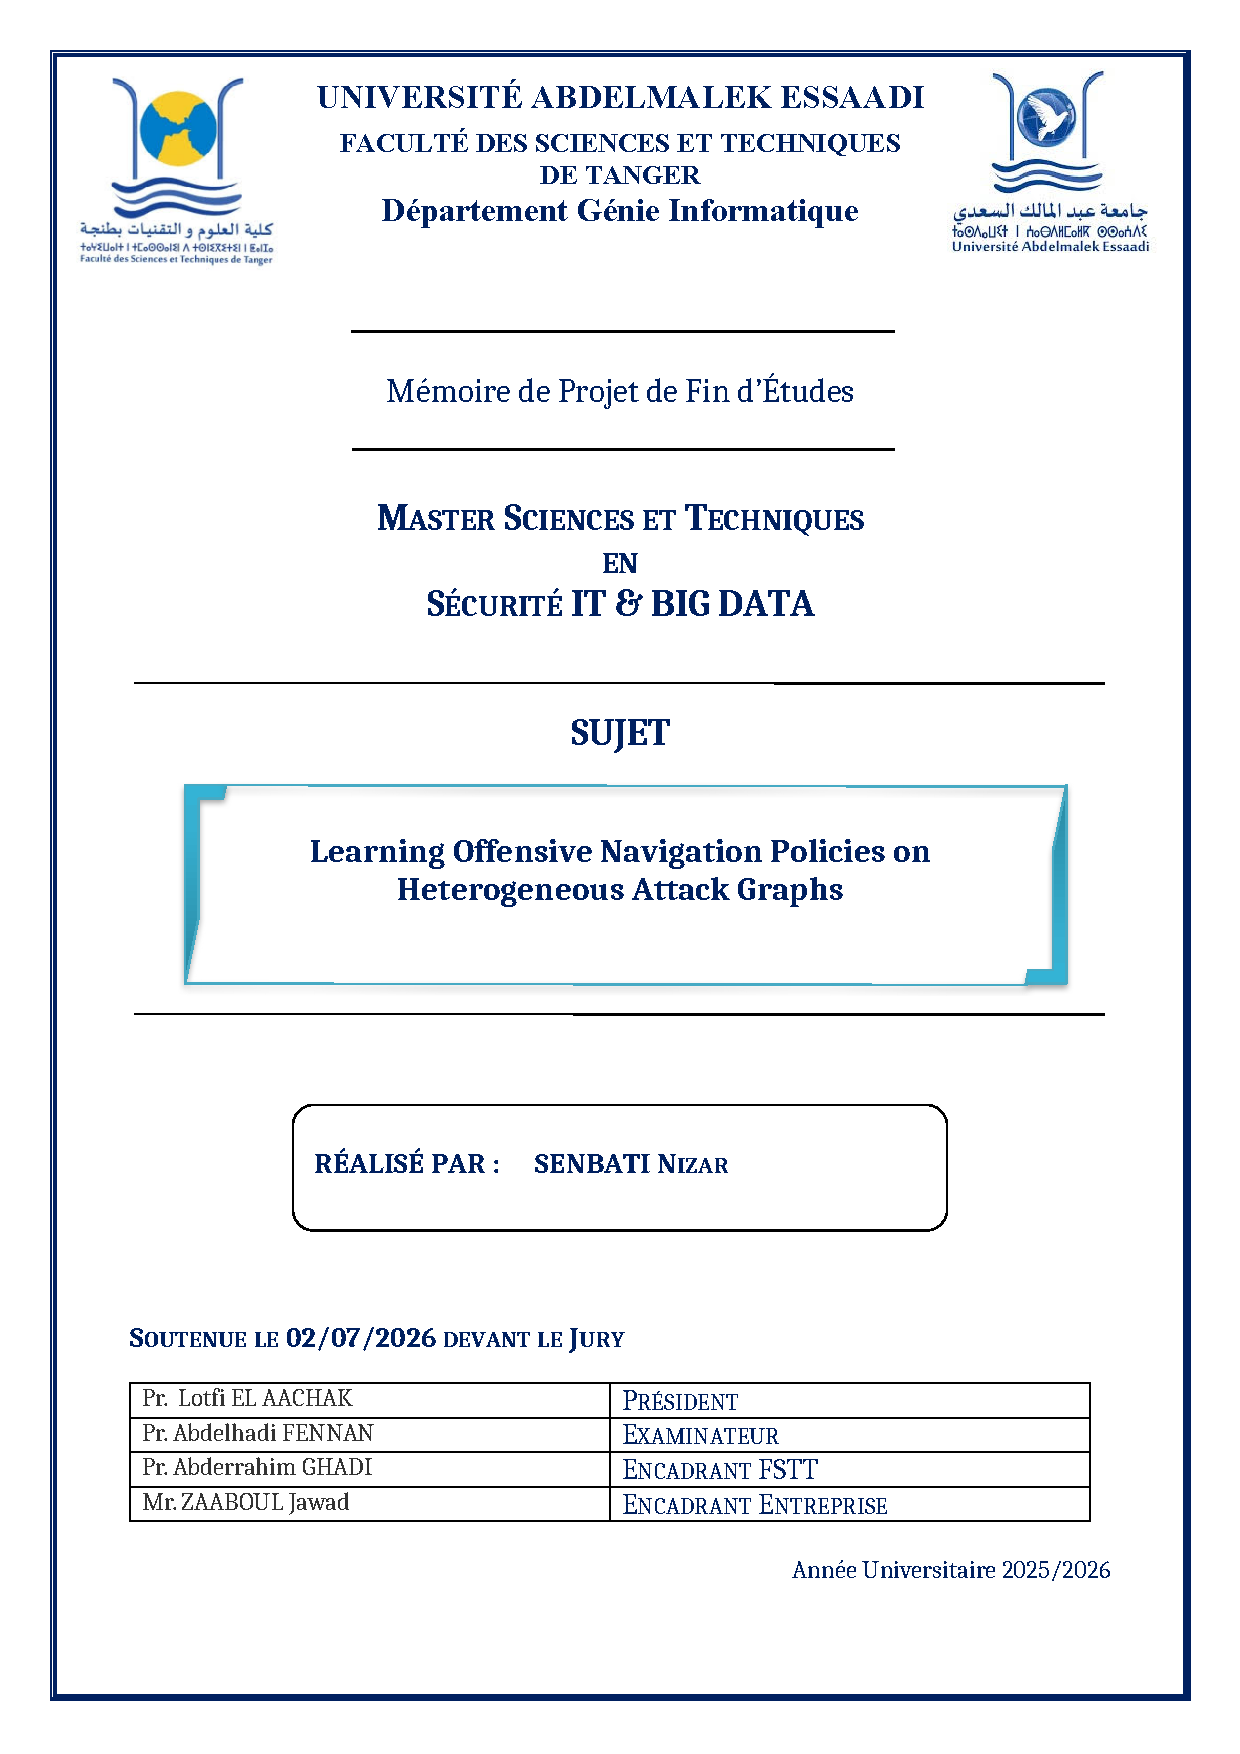
\includepdf[pages={1}]{ressources/page_de_garde.pdf}

% %% ── TITLE PAGE ───────────────────────────────────────────────
% \begin{titlepage}
%   \centering
%   
\includegraphics[width=0.35\textwidth]{ressources/fst_logo.png}\\[1cm]
%   % Replace fst_logo with your actual logo filename (no extension needed if .png/.pdf)

%   {\large\bfseries Faculté des Sciences et Techniques de Tanger}\\[0.3cm]
%   {\large Université Abdelmalek Essaadi}\\[0.5cm]
%   \rule{\textwidth}{0.5pt}\\[0.5cm]

%   {\large Master's End-of-Study Project (PFE)}\\
%   {\large Master in \todo{your master programme name}}\\[1.5cm]

%   {\Huge\bfseries\color{thesisblue}
%     Learning Offensive Navigation Policies\\
%     on Heterogeneous Attack Graphs}\\[0.8cm]

%   {\Large A GNN Approach to Sequential Privilege Escalation\\
%     in Active Directory}\\[2cm]

%   \begin{minipage}[t]{0.45\textwidth}
%     \raggedright
%     \textbf{Author:}\\
%     Nizar Senbati
%   \end{minipage}
%   \hfill
%   \begin{minipage}[t]{0.45\textwidth}
%     \raggedleft
%     \textbf{Supervisor:}\\
%     \todo{Supervisor name \& title}
%   \end{minipage}\\[2cm]

%   \rule{\textwidth}{0.5pt}\\[0.5cm]
%   {\large Academic Year 2025 -- 2026}
% \end{titlepage}

%% ── FRONT MATTER ─────────────────────────────────────────────
\pagenumbering{roman}
\setcounter{page}{1}

%% ── Acknowledgements ─────────────────────────────────────────
\chapter*{Acknowledgements}
\addcontentsline{toc}{chapter}{Acknowledgements}

First and foremost, I would like to express my deepest gratitude to my academic supervisor
GHADI Abderahim, for his unwavering guidance, patience, and invaluable feedback
throughout this academic year.
\\
I am equally grateful to my professional supervisor, ZAABOUL Jawad, and the 
entire team at NearSecure. Thank you for providing an environment that fosters innovation, 
for trusting me to pursue the intersection of offensive security and Deep Learning, 
and for the technical mentorship that bridged the gap between academic theory and real-world application.
\\
A massive thank you is owed to the broader cybersecurity and open-source communities. 
The development of the GNN-AD-Navigator would not have been possible without the tireless 
work of the developers who build and maintain the tools we rely on. Specifically, I would like to acknowledge:
\\
SpecterOps, for creating and open-sourcing BloodHound, which provided the foundational graph 
topology and data schema necessary for my model's ingestion pipeline.
\\
Oliver Lyak ly4k, for developing Certipy, an essential tool that allowed me to accurately 
map complex Active Directory Certificate Services ADCS attack paths into my heterogeneous graph.
\\
Mayfly Orange Cyberdefense, for creating GOAD Game of Active Directory. The immense complexity 
of this lab environment served as the perfect training ground for the neural network, allowing it 
to learn and discover emergent tactical behaviors.
\\
I also want to thank Hack The Box Academy for their student program, which granted me 
accessible access to the inlanefreight Active Directory environment. This provided the critical 
cross-environment validation required to prove the model's efficacy outside of its training data.
\\
Finally, a personal thank you to my father and familly for the ongoing support, advice and guidance during 
the long hours spent debugging and studying. 
To everyone who supported me through this Master's journey: thank you.

%% ── Abstract (English) ───────────────────────────────────────
\chapter*{Abstract}
\addcontentsline{toc}{chapter}{Abstract}

% ~150 words. Cover: problem (AD attack path analysis), approach (GNN policy on
% heterogeneous graph), key result (cross-environment generalisation on INLANEFREIGHT),
% contribution (learned policy vs. shortest path), and honest scope (PoC).
Active Directory is a directory service so deeply embedded in corporate 
infrastructure that misconfigurations, no matter how small, can expose 
entire organisations to privilege escalation attacks. Tools like BloodHound 
are critical for both defenders and red teams: they map the environment as a 
graph and let operators query attack paths between any two objects. 
BloodHound's built-in pathfinding, however, runs plain Dijkstra --- it returns 
the shortest path, not necessarily the most operationally sound one, and it 
cannot learn from prior engagements.

This thesis asks whether a Graph Neural Network can learn a navigation policy 
from labelled attack traces and generalise it to entirely unseen enterprise 
environments. A Heterogeneous Graph Transformer is trained on a multi-domain 
lab environment and evaluated on a 4\,000-node enterprise network it has 
never seen. The model recovers the expert-documented Domain Admin attack path 
without retraining, establishing cross-environment generalisation as a proof 
of concept. Identified architectural boundaries and a forward-looking 
hypothesis for a second-generation tool are discussed.

\vspace{1.5cm}
\noindent\textbf{Keywords:} Graph Neural Network, Heterogeneous Graph Transformer,
Active Directory, Privilege Escalation, Attack Graph, Beam Search,
Offensive Security, Cross-Environment Generalisation, Active Directory Cerfication Services.

%% ── Abstract (French) ────────────────────────────────────────
\chapter*{Résumé}
\addcontentsline{toc}{chapter}{Résumé}

Active Directory est un service d'annuaire si profondément intégré dans l'infrastructure 
des entreprises que la moindre erreur de configuration peut exposer une organisation entière 
à des attaques de privilege escalation. Des outils comme BloodHound sont essentiels 
à la fois pour les défenseurs et les red teams : ils cartographient l'environnement sous forme 
de graphe et permettent aux opérateurs de rechercher des chemins d'attaque entre deux objets.
Cependant, le moteur de recherche de BloodHound utilise le simple algorithme de Dijkstra 
renvoie le chemin le plus court, et non le plus pertinent d'un point de vue opérationnel.

Cette thèse cherche à savoir si un Graph Neural Network peut apprendre une politique de navigation
à partir de traces d'attaques étiquetées, et la généraliser à des environnements d'entreprise 
totalement inconnus. Un Heterogeneous Graph Transformer est entraîné sur un environnement de 
laboratoire multi-domaines, puis évalué sur un réseau d'entreprise de 4 000 nœuds qu'il 
n'a jamais vu auparavant. Le modèle parvient à retrouver le chemin d'attaque Domain Admin 
documenté par des experts, et ce sans réentraînement, validant ainsi la généralisation 
cross-environment comme un véritable Proof of Concept. Enfin, les limites architecturales 
identifiées ainsi que des pistes d'évolution pour un outil de seconde génération sont discutées.

\vspace{1.5cm}
\noindent\textbf{Mots-clés :} Réseau de neurones sur graphe, Transformateur de graphe hétérogène,
Active Directory, Escalade de privilèges, Graphe d'attaque, Recherche en faisceau,
Sécurité offensive, Généralisation inter-environnements.

%% ── Tables of Contents / Figures / Tables ────────────────────
\tableofcontents
\listoffigures
\listoftables

%% ── Abbreviations (auto-generated from glossaries) ──────────
\printglossary[type=\acronymtype, title=List of Abbreviations]

\cleardoublepage
\pagenumbering{arabic}
\setcounter{page}{1}

%% ============================================================
%%  GENERAL INTRODUCTION
%% ============================================================
\chapter*{General Introduction}
\addcontentsline{toc}{chapter}{General Introduction}
\markboth{General Introduction}{}

\section*{Context}

Active Directory is the identity backbone of major enterprises. While typically isolated withing 
the inside network, once the perimeter defenses are breached 
(e.g., via web service exploitation, phishing, or a compromised usb) an advarsary gains the 
ability to directly interacte and query the Active Directory Domain Controller. Through protocols
such as LDAP and SMB the entirety  of the organisation's IT infrastructure , data and services 
is essencialy mapped out for the attacker.
A vulnerable AD poses extreme levels of risk making hardening the AD network environment an extreme priority.


Once inside, attackers frequently leverage credential-based and ACL-based attacks such as 
pass-the-hash, DCSync, Kerberoasting are among the most impactful attack vectors in modern breaches.
Red teams and security auditor alike rely on tools like BloodHound 
to map the attack surface and identify the vulnerable nodes during an engagement. However the analysis remains
a highly manual process, time consuming, heavely depandent on human expertise and none scalable 
in large enterprise environments.


\section*{Problem Statement}

Bloodhound maps the entirety of the Active Directory to a graph database, each node represents an object,
and the relationships between these objects is represented by edges.
When a user runs a path finding query, BloodHound simply runs Dijkstra over the attack graph,
it finds the shortest path, not necessarily the most realistic or discreet one.
\\The question this thesis asks : can a model learn a navigation policy and generalise
that policy to an unseen entreprise environment?

\section*{Objectives}

The objectif of this Thesis is to provide a proof of concept for learned attack path discovery 
over heterogeneous Active Directory graphs.
\\To that end this work aims to:

\begin{itemize}
  \item Build an end-to-end pipeline transforming raw BloodHound and Certipy JSON
  to navigable \gls{pyg} \texttt{HeteroData} tensors.
  \item Train a GNN-based navigation policy and demonstrate cross-environment generalisation 
  to unseen entreprise level environments.
  \item Identify and precisely describe the model's limitations and architectural boundaries 
  through systematic evaluation, establishing future work and improvements.
\end{itemize}


\section*{Main Contributions}
\begin{itemize}
  \item A complete, modular heterogeneous graph pipeline from raw BloodHound/Certipy
        JSON to navigable \gls{pyg} \texttt{HeteroData} tensors, covering
        \gls{adcs}, \gls{rbcd}, GPLink, and \gls{sid} history edges.
  \item A \gls{hgt}-based navigation policy trained on \gls{goad} traces and
        evaluated on the entirely unseen INLANEFREIGHT enterprise environment,
        demonstrating generalisation from a 351-node lab to a 4\,000-node network.
  \item An evaluation of the tool's current limitations. Identifying how the search algorithm 
  naturally penalizes long paths, which creates an unintended bias toward shorter, noisier attacks rather 
  than longer, stealthier desired routes. A highlight of the model's limited line of sight \/
  receptive field when trying to discover deep, multi-step continuous attack chains. Also  
  acknowledging that testing was restricted to lab environments rather than enterprise networks 
  due to time and resource constraints.
  
  \item A proposal for a future, second-generation tool that addresses these limitations by: 
  implementing a guided search algorithm (such as A-Star) to help the model value stealth and 
  keep long attack paths alive; using natural language AI to read and understand entirely new 
  types of attacks based on their descriptions instead of relying on a hardcoded list; and adding 
  a time dimension to the graph to accurately reflect temporary network states, such as active user 
  sessions that log on and off. An automated "divide-and-conquer" routing system that breaks 
  excessively long attack chains into smaller manageable segments using major network hubs or 
  domain boundaries as checkpoints.
\end{itemize}

\section*{Report Outline}
The remainder of this document is structured as follows. 

Chapter 1 establishes the theoretical foundation, reviewing the architecture 
of Active Directory, common privilege escalation techniques, the machine 
learning logic behind GNNs, and the current state of graph-based attack 
path analysis.

Chapter 2 details the methodology and system architecture, introducing the 
heterogeneous graph pipeline designed to transform raw BloodHound data into 
navigable tensors. It also presents the core logic of the navigation policy, 
the loss function, and the beam search method.

Chapter 3 presents the internal architecture and the training paradigm of 
the Graph Neural Network GNN navigation policy.

Chapter 4 provides an empirical evaluation of the learned policy across 
multiple environments, documenting both successful generalizations and 
precise failure modes. It evaluates the tool's current limitations, 
specifically identifying how the search algorithm naturally penalizes 
long paths (creating a bias toward shorter, noisier attacks) and defining 
the model's limited receptive field when navigating deep attack chains.

Chapter 5 concludes the report by reviewing the achievements of this proof 
of concept and honestly assessing its limitations. It then proposes a 
second-generation tool featuring practical engineering improvements, such 
as automated waypoint routing to chunk long paths, guided search algorithms 
to prioritize stealth, and the integration of natural language models to 
dynamically interpret novel attack techniques.


%% ============================================================
%%  CHAPTER 1 — BACKGROUND AND RELATED WORK
%% ============================================================
\chapter{Background and Related Work}

\section{Active Directory: Architecture and Security Model}

\subsection{Core Objects and Structure}
% Cover: users, computers, OUs, GPOs, domains, forests, trusts.
% One diagram of the hierarchical AD structure (forest → domain → OU → objects)
% is worth inserting here.

Active Directory (AD) a directory service for Windows network environments. It is a distributed, 
hierarchical structure that allows for centralized management of an organization's resources, 
including users, computers, groups, network devices, file shares, group policies, servers 
and workstations, and trusts. AD provides authentication and authorization functions within 
a Windows domain environment.\cite{htbacademy}
\\
\\
\begin{figure}[H]
  \centering
  \textbf{\color{navyblue} Active Directory Object Hierarchy} \\[0.5em]
  \resizebox{\textwidth}{!}{%
  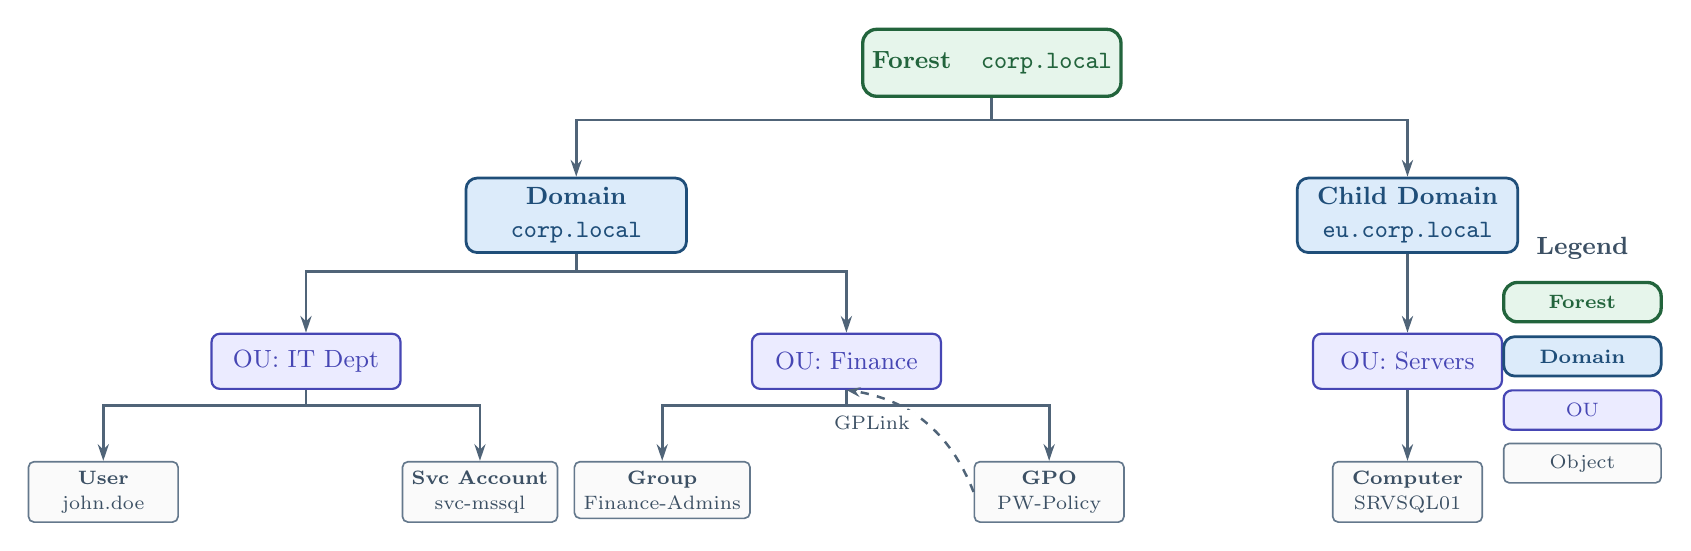
\begin{tikzpicture}[node distance=0.5cm and 0.5cm]

  %\node[diagramtitle] (T) {Active Directory Object Hierarchy};

  %% Forest
  \node[forestbox, below=0.7cm] (forest)
    {Forest\quad\texttt{corp.local}};

  %% Domains
  \node[domainbox, below left=1.0cm and 2.2cm of forest] (d1)
    {Domain\\[1pt]\texttt{corp.local}};
  \node[domainbox, below right=1.0cm and 2.2cm of forest] (d2)
    {Child Domain\\[1pt]\texttt{eu.corp.local}};

  \draw[thesisarrow] (forest.south) -- ++(0,-0.28) -| (d1.north);
  \draw[thesisarrow] (forest.south) -- ++(0,-0.28) -| (d2.north);

  %% OUs under d1
  \node[oubox, below left=1.0cm and 0.8cm of d1] (ou1) {OU: IT Dept};
  \node[oubox, below right=1.0cm and 0.8cm of d1] (ou2) {OU: Finance};

  \draw[thesisarrow] (d1.south) -- ++(0,-0.22) -| (ou1.north);
  \draw[thesisarrow] (d1.south) -- ++(0,-0.22) -| (ou2.north);

  %% OU under d2
  \node[oubox, below=1.0cm of d2] (ou3) {OU: Servers};
  \draw[thesisarrow] (d2.south) -- (ou3.north);

  %% Objects under ou1
  \node[objbox, below left=0.9cm and 0.4cm of ou1] (u1)
    {\textbf{User}\\[1pt]john.doe};
  \node[objbox, below right=0.9cm and 0cm of ou1] (s1)
    {\textbf{Svc Account}\\[1pt]svc-mssql};

  \draw[thesisarrow] (ou1.south) -- ++(0,-0.2) -| (u1.north);
  \draw[thesisarrow] (ou1.south) -- ++(0,-0.2) -| (s1.north);

  %% Objects under ou2
  \node[objbox, below left=0.9cm and 0cm of ou2] (g1)
    {\textbf{Group}\\[1pt]Finance-Admins};
  \node[objbox, below right=0.9cm and 0.4cm of ou2] (gpo)
    {\textbf{GPO}\\[1pt]PW-Policy};

  \draw[thesisarrow] (ou2.south) -- ++(0,-0.2) -| (g1.north);
  \draw[thesisarrow] (ou2.south) -- ++(0,-0.2) -| (gpo.north);

  %% Objects under ou3
  \node[objbox, below=0.9cm of ou3] (c1)
    {\textbf{Computer}\\[1pt]SRVSQL01};
  \draw[thesisarrow] (ou3.south) -- (c1.north);

  %% GPLink dashed
  \draw[dasharrow, bend right=30] (gpo.west)
    to node[arrowlabel, left=3pt] {GPLink} (ou2.south);

  %% Legend
  \begin{scope}[shift={(7.5,-3.5)}]
    \node[font=\small\bfseries\color{labelgray}] (lt) {Legend};
    \node[forestbox, minimum width=2.0cm, minimum height=0.5cm,
          font=\scriptsize\bfseries\color{forestgreen},
          below=0.15cm of lt] (ll1) {Forest};
    \node[domainbox, minimum width=2.0cm, minimum height=0.5cm,
          font=\scriptsize\bfseries\color{navyblue},
          below=0.15cm of ll1] (ll2) {Domain};
    \node[oubox, minimum width=2.0cm, minimum height=0.5cm,
          font=\scriptsize\color{oucolor},
          below=0.15cm of ll2] (ll3) {OU};
    \node[objbox, minimum width=2.0cm, minimum height=0.5cm,
          below=0.15cm of ll3] (ll4) {Object};
  \end{scope}

\end{tikzpicture}
}
  \caption{Active Directory object hierarchy.}
  \label{fig:active-directory-hierarchy}
\end{figure}

Figure 1.1 illustrates the standard hierarchical structure of an Active 
Directory environment. At the highest level is the Forest, which serves 
as the absolute security boundary for the organization. Within the forest, 
one or more Domains act as logical partitions to manage resources. To 
streamline administration, these domains are further subdivided into 
Organizational Units OUs. OUs act as geographical or functional 
containers to group specific base objects, such as users, 
service accounts, security groups, and computers. Additionally, the 
diagram highlights how Group Policy Objects GPOs can be linked directly 
to OUs to enforce specific security configurations across all objects 
within that container.

By design, Active Directory allows almost any authenticated user regardless 
of their administrative privilege level to read and query the directory. 
This open read-access is intended to facilitate normal network operations, 
such as allowing a user to look up a colleague's email address or locate a 
network printer. However, this feature creates a significant security 
vulnerability. 

If an adversary compromises a single, unprivileged user account or workstation, 
they can abuse this read access using standard protocols like LDAP and RPC. 
The attacker can silently sweep the directory to extract the exact same list 
of computers, group memberships, trust relationships, and Access Control 
Lists (ACLs) detailed above. By stitching this data together, the adversary 
can map the entire network topology and identify hidden, multi-step privilege 
escalation paths leading from their starting point to high-value targets 
like Domain Admin.

Because the relationships between thousands of Active Directory objects create 
a highly complex web of permissions, manually identifying these chained 
vulnerabilities is nearly impossible. To address this, security professionals, 
defenders, and penetration testers utilize graph-based pathfinding tools. 
By ingesting the same directory data that an attacker would enumerate, these 
tools model the Active Directory environment as a mathematical graph. This 
allows operators to visualize hidden attack paths, proactively identify 
structural weaknesses, and remediate dangerous permission chains before they 
can be exploited during a real breach.

A standard Active Directory user account with no administrative privileges can be leveraged 
to query and enumerate a vast amount of structural and security data across the network. 
This accessible information includes, but is not limited to:

\begin{itemize}
  \setlength{\itemsep}{0pt}
  \setlength{\parskip}{0pt}
  \item Domain Computers
  \item Domain Group Information
  \item Default Domain Policy
  \item Password Policy
  \item Domain Trusts
  \item Domain Users
  \item Organizational Units (OUs)
  \item Functional Domain Levels
  \item Group Policy Objects (GPOs)
  \item Access Control Lists (ACLs)
\end{itemize}


\subsection{Authentication Protocols}
\label{sec:auth_protocols}

Active Directory manages network security through the fundamental AAA 
framework: Authentication, Authorization, and Accounting 
\cite{microsoft_ad_sec}. When a user, machine, or service attempts to 
access a network resource, AD first verifies their cryptographic 
identity (Authentication). Once identity is proven, the system evaluates 
the user's embedded Security Identifier (SID) and group memberships 
against the target resource's Access Control Lists (Authorization). 
Finally, the Domain Controller logs the logon events and access requests 
(Accounting) to ensure auditability. To execute the initial authentication 
phase, Active Directory relies primarily on two distinct network 
protocols: Kerberos and NTLM.

\subsubsection*{Kerberos}
Kerberos is the default and preferred authentication protocol in modern 
Active Directory environments \cite{rfc4120}. It operates as a 
sophisticated, ticket-based system brokered by a Key Distribution Center 
(KDC), a service that runs natively on every Domain Controller. Rather 
than transmitting passwords or hashes across the network, Kerberos relies 
on symmetric-key cryptography. Upon a successful initial logon, the KDC 
issues the client a Ticket Granting Ticket (TGT). When the client needs 
to access a specific network service (such as a file share or database), 
it presents the TGT to the KDC to request a Service Ticket (ST) for that 
specific resource. While Kerberos relies on strict timestamping to 
prevent replay attacks and is cryptographically robust, its complex 
delegation and ticketing mechanics make it a primary target for advanced 
adversaries who abuse it via techniques such as Pass-the-Ticket, Golden 
Tickets, and delegation hijacking.

\begin{figure}[H]
  \centering
  \textbf{\color{navyblue} Kerberos Authentication Flow} \\[0.5em]
  \resizebox{\textwidth}{!}{%
  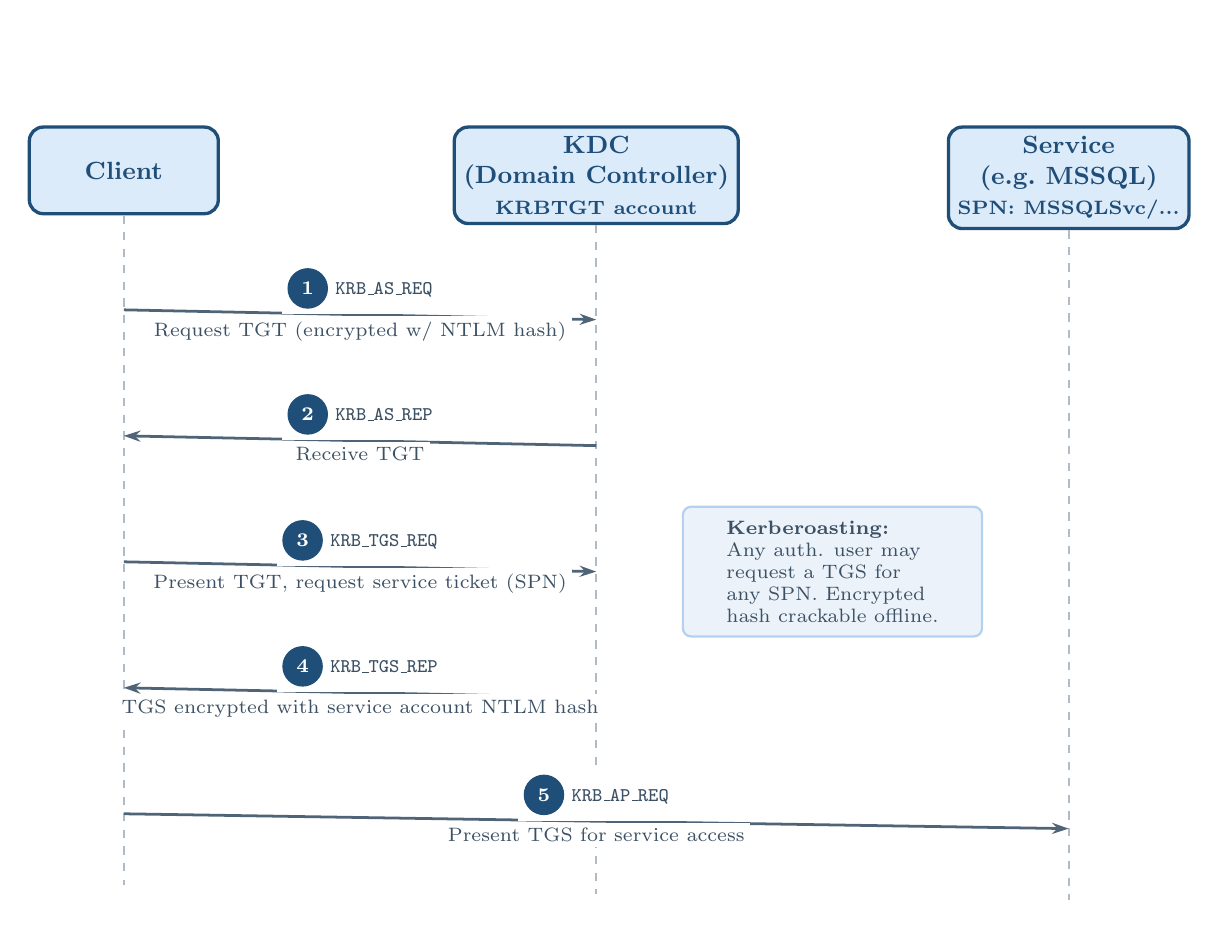
\begin{tikzpicture}[node distance=2.5cm and 0.8cm]

  \node[diagramtitle] (T) {};

  %% Entities
  \node[entitybox, below=1.0cm of T, xshift=-6.0cm] (kc)
    {Client};
  \node[entitybox, below=1.0cm of T] (kdc)
    {KDC\\(Domain Controller)\\{\scriptsize KRBTGT account}};
  \node[entitybox, below=1.0cm of T, xshift=6.0cm] (ksvc)
    {Service\\(e.g.\ MSSQL)\\{\scriptsize SPN: MSSQLSvc/...}};

  %% Lifelines
  % Extended to -8.5 to accommodate all arrows and text
  \draw[draw=slategray!50, dashed, thick]
    (kc.south) -- ++(0,-8.5);
  \draw[draw=slategray!50, dashed, thick]
    (kdc.south) -- ++(0,-8.5);
  \draw[draw=slategray!50, dashed, thick]
    (ksvc.south) -- ++(0,-8.5);

  %% 1 AS-REQ
  \draw[thesisarrow]
    ([yshift=-1.2cm]kc.south) -- ([yshift=-1.2cm]kdc.south)
    node[arrowlabel, above, midway] {\stepnum{1}~\texttt{KRB\_AS\_REQ}}
    node[arrowlabel, below, midway] {Request TGT (encrypted w/ NTLM hash)};

  %% 2 AS-REP
  \draw[thesisarrow]
    ([yshift=-2.8cm]kdc.south) -- ([yshift=-2.8cm]kc.south)
    node[arrowlabel, above, midway] {\stepnum{2}~\texttt{KRB\_AS\_REP}}
    node[arrowlabel, below, midway] {Receive TGT};

  %% 3 TGS-REQ
  \draw[thesisarrow]
    ([yshift=-4.4cm]kc.south) -- ([yshift=-4.4cm]kdc.south)
    node[arrowlabel, above, midway] {\stepnum{3}~\texttt{KRB\_TGS\_REQ}}
    node[arrowlabel, below, midway] {Present TGT, request service ticket (SPN)};

  %% 4 TGS-REP
  \draw[thesisarrow]
    ([yshift=-6.0cm]kdc.south) -- ([yshift=-6.0cm]kc.south)
    node[arrowlabel, above, midway] {\stepnum{4}~\texttt{KRB\_TGS\_REP}}
    node[arrowlabel, below, midway] {TGS encrypted with service account NTLM hash};

  %% 5 AP-REQ client→service
  % Now perfectly bridges from the Client lifeline directly to the Service lifeline
  \draw[thesisarrow]
    ([yshift=-7.6cm]kc.south) -- ([yshift=-7.6cm]ksvc.south)
    node[arrowlabel, above, midway] {\stepnum{5}~\texttt{KRB\_AP\_REQ}}
    node[arrowlabel, below, midway] {Present TGS for service access};

  %% Annotation: Kerberoasting
  % Positioned exactly halfway between KDC and Service (xshift=3.0cm)
  \node[msgbox, minimum width=3.8cm, align=left] at ([xshift=3.0cm, yshift=-4.4cm]kdc.south) {
    \textbf{Kerberoasting:}\\
    Any auth. user may\\
    request a TGS for\\
    any SPN. Encrypted\\
    hash crackable offline.
  };

  \end{tikzpicture}%
  } 
  \caption{Kerberos Authentication Flow}
  \label{fig:kerberos-auth}
\end{figure}

Within the specific context of this thesis, two Kerberos-related dynamics 
are of critical offensive relevance. First, Constrained Delegation allows 
a service to request a Service Ticket on behalf of any user. This abuse 
primitive is captured by our data extraction pipeline as an 
\edge{AllowedToDelegate} edge, enabling the highly stealthy privilege 
escalation chains that our model learns to navigate. Second, while 
Kerberos secures standard authentication, ultimate domain compromise often 
bypasses ticket exchanges entirely. For instance, the DCSync attack 
leverages \edge{GetChanges} and \edge{GetChangesAll} replication rights 
to extract NTLM hashes directly from the Domain Controller without ever 
interacting with the Kerberos KDC.

\subsubsection*{NT LAN Manager (NTLM)}
NT LAN Manager (NTLM) is a legacy suite of Microsoft security protocols 
that remains widely enabled in Active Directory environments, primarily 
to ensure backwards compatibility with older clients or poorly configured 
applications. Unlike the ticket-brokered architecture of Kerberos, NTLM 
utilizes a direct challenge-response mechanism. When a client attempts 
to authenticate to a server, the server issues a random challenge. The 
client then encrypts this challenge using the NTLM hash of the user's 
password and returns it to prove their identity. Because NTLM lacks 
mutual authentication and transmits cryptographic material in a 
predictable challenge-response format, it is inherently weaker than 
Kerberos. Offensively, NTLM is frequently targeted for exploitation 
through hash extraction (Pass-the-Hash) and network interception 
(NTLM Relay attacks).

\subsection{Trust Relationships}
\label{sec:trust_relationships}

In large enterprise environments, organizations frequently span multiple 
domains or even entirely separate Active Directory forests. To allow 
users in one domain to access resources located in another, Active 
Directory employs a mechanism known as Trust Relationships 
\cite{microsoft_ad_sec}. A trust acts as a secure cryptographic bridge 
between two boundaries. These relationships can be configured as 
one-way, where Domain A trusts Domain B (but not vice versa), or 
two-way, where both domains trust each other equally. Furthermore, 
trusts can be transitive---meaning the trust flows through a chain 
of domains---or non-transitive, restricting the relationship strictly 
to the two interacting domains. As illustrated in the diagram below, 
these trust links can occur between child and parent domains within 
the same forest, or across entirely different corporate forests.

\begin{figure} [H]
  \centering
  \textbf{\color{navyblue} Forest and Trust Relationships} \\[0.5em]
  \resizebox{\textwidth}{!}{%
  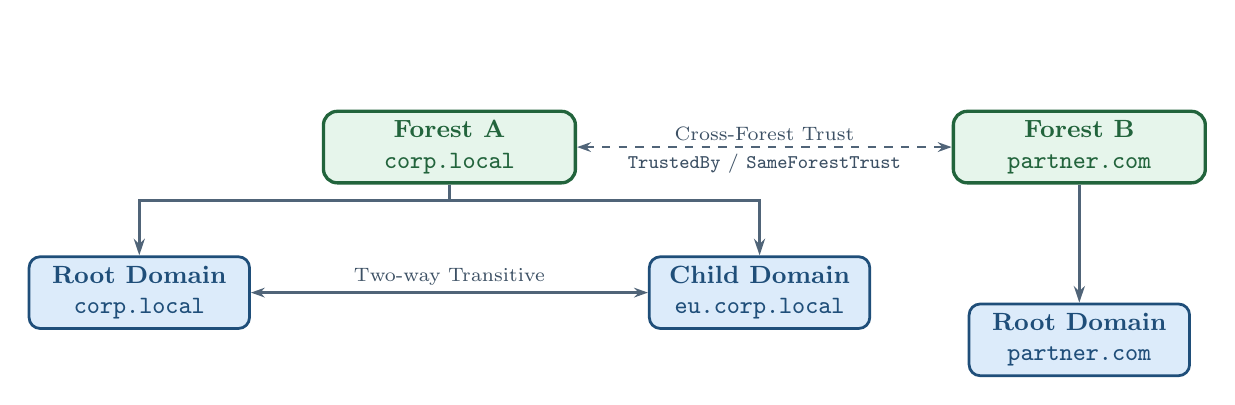
\begin{tikzpicture}[node distance=0.9cm and 1.8cm]
    \node[diagramtitle] (T) {};

    %% Forest A
    \node[forestbox, below=0.8cm of T, xshift=-4.0cm] (fA)
      {Forest A\\\texttt{corp.local}};
    \node[domainbox, below left=0.9cm and 0.9cm of fA] (dA1)
      {Root Domain\\\texttt{corp.local}};
    \node[domainbox, below right=0.9cm and 0.9cm of fA] (dA2)
      {Child Domain\\\texttt{eu.corp.local}};

    \draw[thesisarrow] (fA.south) -- ++(0,-0.2) -| (dA1.north);
    \draw[thesisarrow] (fA.south) -- ++(0,-0.2) -| (dA2.north);

    \draw[bidiarrow] (dA1.east) -- (dA2.west)
      node[arrowlabel, above, midway] {Two-way Transitive};

    %% Forest B
    \node[forestbox, below=0.8cm of T, xshift=4.0cm] (fB)
      {Forest B\\\texttt{partner.com}};
    \node[domainbox, below=1.5cm of fB] (dB1)
      {Root Domain\\\texttt{partner.com}};
    \draw[thesisarrow] (fB.south) -- (dB1.north);

    %% Cross-forest trust
    \draw[bidiarrow, dashed]
      (fA.east) -- (fB.west)
      node[arrowlabel, above, midway] {Cross-Forest Trust}
      node[arrowlabel, below, midway] {\texttt{TrustedBy} / \texttt{SameForestTrust}};

    %% Annotation
  %  \node[msgbox, below=3.5cm of T, minimum width=7.5cm] (note) {
  %    \textbf{BloodHound edge naming inconsistency:} SharpHound versions\\
  %    differ in how they label trust edges (\texttt{TrustedBy} vs.\\
  %    \texttt{SameForestTrust}). Both are aliased in \texttt{build\_dataset.py}.
  %  };

  \end{tikzpicture}
} 
  \caption{Active Directory Trust relationships.}
  \label{fig:ad-hierarchy}
\end{figure}

While trust relationships are essential for administrative flexibility 
and resource sharing, they introduce complex attack vectors when 
misconfigured or overly permissive \cite{harmj0y_trusts}. Adversaries 
frequently abuse bidirectional transitive trusts to move laterally 
across an entire forest boundary. For instance, if an attacker 
compromises a loosely secured child domain, they can forge an 
inter-realm ticket or abuse the SID History attribute to escalate 
privileges to the parent root domain, effectively compromising the 
entire forest. Similarly, poorly audited cross-forest trusts can 
inadvertently grant external users excessive permissions. This allows 
an attacker who compromises a partner organization's network to pivot 
seamlessly into the primary corporate environment. Consequently, mapping 
and analyzing these trust links is a critical component of assessing 
an organization's true security perimeter.

% ─────────────────────────────────────────────────────────────
\section{Privilege Escalation in AD Environments}

\subsection{Offensive ACL Abuse}
\label{sec:acl_abuse}

Access Control Lists (ACLs) serve as the granular security foundation of 
Active Directory, defining exactly which principals have specific permissions 
over directory objects. Historically, defenders focused primarily on network 
vulnerabilities or missing software patches. However, modern offensive 
tradecraft has demonstrated that abusing misconfigured ACLs is often the 
most common, reliable, and critical path for privilege escalation within an 
enterprise environment \cite{specterops_ace}. 

Because ACL misconfigurations allow attackers to subvert the intended 
security architecture seamlessly without triggering traditional malware 
alerts, mapping these specific permissions is the primary function of 
data collection tools like BloodHound. Consequently, these structural 
ACL relationships form the foundational dataset that the GNN-AD-Navigator 
pipeline extracts. Our model heavily bases its recommended paths on these 
extracted rights, learning to weigh the operational cost of exploiting 
each specific permission.

When an adversary compromises a basic account, they enumerate the 
directory to identify objects where their controlled principal holds 
abusive rights. The most critical offensive ACL primitives include:

\begin{itemize}
  \item \textbf{GenericAll:} This right grants complete, unrestricted 
  control over the target object. An attacker holding \texttt{GenericAll} 
  can execute any action, such as adding a user to a highly privileged 
  group, resetting an account's password, or modifying critical attributes 
  to establish persistence.
  
  \item \textbf{WriteDACL:} This permission allows a principal to modify 
  the target object's access control list itself. From an offensive 
  perspective, an attacker can abuse \texttt{WriteDACL} to simply grant 
  themselves \texttt{GenericAll} privileges, effectively taking full 
  control of the target in a two-step process.
  
  \item \textbf{GenericWrite:} While not providing full control, this right 
  allows an attacker to update specific properties of an object. It is 
  frequently weaponized to modify the \texttt{servicePrincipalName} (SPN) 
  attribute to enable targeted Kerberoasting, or to alter the 
  \texttt{msDS-AllowedToActOnBehalfOfOtherIdentity} attribute to execute 
  Resource-Based Constrained Delegation (RBCD) attacks.
  
  \item \textbf{ForceChangePassword:} This specific permission allows an 
  attacker to reset the password of a target user without knowing the 
  current password. While highly effective for immediately compromising an 
  account and hijacking its session, it is operationally ``loud.'' It 
  disrupts the legitimate user's access, making it highly detectable by 
  defenders.
  
  \item \textbf{AddMember:} If held over a security group, this right 
  allows an attacker to directly append their own controlled account 
  (or another compromised user) into the target group. This immediately 
  grants the attacker all the privileges inherited by that group across 
  the entire domain.
\end{itemize}

\subsection{DCSync Attack}
\label{sec:dcsync}

The DCSync attack is one of the most critical techniques used by 
adversaries to extract credentials from a domain without requiring 
direct code execution on a Domain Controller \cite{mimikatz_dcsync}. 
Active Directory relies on the Directory Replication Service Remote 
Protocol (MS-DRSR) to synchronize data across multiple Domain 
Controllers. To abuse this, an attacker only needs an account that 
holds specific replication permissions---specifically, 
\edge{GetChanges} (Replicating Directory Changes) and 
\edge{GetChangesAll} (Replicating Directory Changes All) at the domain 
root level. 

Once these permissions are acquired, the attacker's machine can 
masquerade as a legitimate Domain Controller and issue a replication 
request. The target DC will respond by transmitting the requested 
account credentials, including the highly sensitive NTLM hash of the 
\texttt{krbtgt} account. Securing these replication rights is often the 
terminal objective in offensive pathfinding operations, as it allows 
for the immediate creation of Golden Tickets and total forest compromise.

\subsection{ADCS Attack Paths}
\label{sec:adcs_paths}

Active Directory Certificate Services (ADCS) is Microsoft's native 
Public Key Infrastructure (PKI) implementation. While it provides 
essential cryptographic functions, misconfigured certificate templates 
introduce devastating escalation vectors \cite{specterops_adcs}. These 
vulnerabilities, famously categorized into escalating scenarios 
(ESC1 through ESC15), often allow an unprivileged user to request a 
certificate on behalf of a highly privileged principal, such as a 
Domain Admin. 

By leveraging the PKINIT protocol, the attacker can use the fraudulently 
obtained certificate to request a Kerberos Ticket Granting Ticket (TGT) 
for the impersonated admin, instantly seizing control of the domain. 
The inclusion of ADCS nodes and edges (such as \edge{Enroll} and 
\edge{ManageCA}) drastically expands the complexity of the Active 
Directory attack graph, presenting massive new navigational challenges 
for automated pathfinding tools.

\subsection{SID History Abuse and RBCD}
\label{sec:sid_rbcd}

Beyond standard access controls, advanced adversaries frequently abuse 
inherent Active Directory features designed for compatibility and 
migration. The \texttt{sIDHistory} attribute, originally intended to 
preserve a user's access rights when migrating between domains, can be 
weaponized. If an attacker compromises a domain, they can inject the 
Security Identifier (SID) of a highly privileged group (such as 
Enterprise Admins) into an account's \texttt{sIDHistory}. This grants 
the attacker persistent, cross-domain administrative access while 
bypassing standard group membership audits.

Similarly, Resource-Based Constrained Delegation (RBCD) shifts the 
control of delegation from the domain administrator to the target 
resource itself \cite{elad_rbcd}. If an attacker acquires 
\edge{GenericWrite} privileges over a target computer object, they can 
modify its \texttt{msDS-AllowedToActOnBehalfOfOtherIdentity} attribute. 
This modification allows the attacker to authorize a computer they 
already control to impersonate any user on the compromised target, 
effectively granting them full administrative access to the machine. 
Because RBCD relies on targeted attribute modification rather than 
global delegation rights, it represents a stealthy and highly effective 
edge in modern attack graphs.

\section{Existing Tools and Their Limitations}

\subsection{BloodHound and SharpHound}
\label{sec:bloodhound}

BloodHound has become the de facto industry standard for visualizing and 
analyzing Active Directory security structures \cite{bloodhound_repo}. 
Operating on a Neo4j graph database backend, BloodHound ingests data 
collected by its C\# ingestor, SharpHound, to map relationships between 
users, computers, and groups. By representing AD components as nodes and 
privileges as edges, BloodHound allows security professionals to visualize 
complex attack paths that would be impossible to identify manually.

However, BloodHound's primary limitation lies in its routing logic. The 
platform relies heavily on Dijkstra's algorithm to calculate the shortest 
path between an attacker's starting node and their target. In this 
deterministic model, every edge is treated with an equal, unweighted cost 
of one. BloodHound cannot natively distinguish between a highly detectable, 
noisy action (such as forcing a password reset on an active administrator) 
and a highly stealthy vector (such as abusing an \edge{AllowedToDelegate} 
trust). Because it strictly minimizes hop count, the tool frequently 
recommends operationally unviable or easily detectable attack paths, 
leaving a critical gap for context-aware, machine learning-driven routing 
solutions.

\subsection{\texttt{Certipy}}
\label{sec:certipy}

SharpHound historically lacked deep inspection 
capabilities for certificate infrastructure. To address this, \texttt{Certipy} 
was developed as a Python-based equivalent specifically for \gls{adcs}, 
designed for cross-platform and remote execution. Created by Oliver Lyak, 
Certipy is explicitly defined as an ``offensive tool for enumerating and 
abusing Active Directory Certificate Services'' \cite{certipy_pypi}. 
Developed primarily for UNIX-like environments, this tool leverages remote 
queries to extract certificate templates, Certificate Authorities, and 
complex PKI permissions. It is an essential component for attackers operating 
from external infrastructure or non-Windows pivot machines, and it serves 
as the primary \gls{adcs} data collection engine for the pipeline developed 
in this thesis.

\subsection{\texttt{bloodhound-python}}
\label{sec:bh_python}

While SharpHound is designed to be executed directly from a compromised 
Windows host, \texttt{bloodhound-python} serves as its Python-based 
equivalent, designed for cross-platform and remote execution 
\cite{bloodhound_python}. Developed primarily for UNIX-like environments, 
this tool leverages the \texttt{impacket} library to query LDAP and RPC 
remotely. It is an essential component for attackers operating from external 
infrastructure or non-Windows pivot machines, and it serves as the primary 
data collection engine for the pipeline developed in this thesis.

However, \texttt{bloodhound-python} suffers from severe functional 
limitations compared to its C\# counterpart. Most critically, it lacks 
native support for enumerating \gls{adcs} 
templates. To bridge this gap, operators are forced to rely on external 
tooling such as \texttt{Certipy}. This introduces a fragile dependency 
chain: because Certipy officially retired BloodHound integration in its 
v5.0.0 release, operators must intentionally downgrade and maintain legacy 
versions (e.g., v4.3.0) strictly for dataset compatibility \cite{certipy_repo}.

Furthermore, \texttt{bloodhound-python} exhibits blind spots in complex 
enterprise architectures, notably struggling to accurately map specific 
cross-domain trust accounts. Because its default implementation relies on 
static and often lagging extraction logic, the ingestor will blindly bypass 
novel misconfigurations or unmapped edge types unless its underlying parsing 
code is manually updated. This effectively blinds any downstream pathfinding 
algorithms to those specific routes, cementing the pipeline's extraction 
phase as a critical bottleneck for the overall model.

\subsection{Other Automated Attack Path Tools}
\label{sec:other_tools}

The success of BloodHound has inspired several supplementary tools aimed 
at automating attack path execution and reporting. Tools such as PlumHound 
and GoFetch interact directly with BloodHound's Neo4j database to generate 
human-readable audit reports or to automatically execute the identified 
exploit chains \cite{gofetch}. Similarly, auditing software like PingCastle 
provides rapid, rule-based assessments of Active Directory risk scores by 
flagging known misconfigurations \cite{pingcastle}.

While these tools excel at operationalizing graph data and generating 
compliance reports, they fundamentally inherit the baseline limitations of 
the underlying Neo4j Cypher queries. They do not generate novel paths or 
apply dynamic, environment-specific heuristics to evaluate edge costs. The 
offensive security industry currently lacks a widely adopted tool capable 
of applying heterogeneous attention mechanisms to weigh the semantic value 
of AD relationships. This thesis addresses this exact void by substituting 
deterministic shortest-path algorithms with a \gls{gnn} 
policy capable of learning stealth and operational viability.

% ─────────────────────────────────────────────────────────────
\section{Graph Neural Networks}

\subsection{Message Passing and Neighbourhood Aggregation}
\label{sec:gnn_fundamentals}

Standard deep learning models are generally designed for structured data, 
such as grids of pixels or sequences of text. However, Active Directory (AD) 
environments are highly interconnected and asymmetrical, making them best 
represented as graphs. Graph Neural Networks (GNNs) address this by learning 
directly from the structural relationships between entities in the network.

Let an Active Directory environment be defined as a graph 
$\mathcal{G} = (\mathcal{V}, \mathcal{E})$, where $\mathcal{V}$ represents 
the set of nodes (users, groups, computers) and $\mathcal{E}$ represents 
the set of edges (permissions, trusts, active sessions). The primary 
objective of a GNN is to encode each node into a continuous numerical 
vector, a \textbf{node embedding}. The initial state of a node 
$v \in \mathcal{V}$ is denoted by its starting feature vector, 
$\mathbf{h}_v^{(0)} = \mathbf{x}_v$.

To capture the topology of the network, GNNs rely on a mechanism called 
\textit{message passing}. During this process, each node gathers information 
from its direct neighbours to update its own state. Mathematically, the 
operation at the $k$-th \textbf{hidden layer} consists of an aggregation 
step and an update step. The message collected from the neighbourhood 
$\mathcal{N}(v)$ is defined as:

$$
\mathbf{m}_{\mathcal{N}(v)}^{(k)} = \text{AGGREGATE}^{(k)} \left( \left\{ \mathbf{h}_u^{(k-1)} : u \in \mathcal{N}(v) \right\} \right)
$$

where $\text{AGGREGATE}$ is a mathematical function such as the sum or mean. 
After aggregating this neighbourhood data, the node updates its own 
embedding. It combines its previous state with the newly collected message 
using a learned weight matrix $\mathbf{W}^{(k)}$ and a non-linear activation 
function $\sigma$:

$$
\mathbf{h}_v^{(k)} = \sigma \left( \mathbf{W}^{(k)} \cdot \left( \mathbf{h}_v^{(k-1)} \parallel \mathbf{m}_{\mathcal{N}(v)}^{(k)} \right) \right)
$$

The number of hidden layers, $K$, determines the receptive field of the 
model—meaning how far a node can "see" into the graph. For example, in a 
network with $K=3$ layers, the final embedding $\mathbf{h}_v^{(K)}$ captures 
structural information from nodes up to three hops away.

Once the node embeddings are finalized, they are used to make routing 
decisions during an attack path simulation. This is managed by the 
\textbf{policy head}. Since the number of outbound connections varies 
greatly across AD nodes, the policy head evaluates each potential neighbour 
individually. It concatenates the current node's embedding $\mathbf{h}_v^{(K)}$, 
the candidate neighbour's embedding $\mathbf{h}_u^{(K)}$, and the target 
node's embedding $\mathbf{h}_{\text{target}}^{(K)}$, passing them through a 
Multi-Layer Perceptron (MLP) to generate a raw transition score:

$$
e_{v,u} = \text{MLP} \left( \mathbf{h}_v^{(K)} \parallel \mathbf{h}_u^{(K)} \parallel \mathbf{h}_{\text{target}}^{(K)} \right)
$$

These raw scores are then normalized across all valid neighbours using a 
Softmax function. This produces a valid probability distribution $\pi$ that 
guides the pathfinding algorithm toward the most promising next step:

$$
\pi(u | v) = \frac{\exp(e_{v,u})}{\sum_{w \in \mathcal{N}(v)} \exp(e_{v,w})}
$$

\subsubsection*{The Impact of Graph Size and Density}

While GNNs are highly effective, their performance is closely tied to the 
graph's size and connectivity. In large Active Directory networks, dense 
configurations—such as heavily nested group memberships—can cause 
\textit{neighbourhood explosion}. This drastically increases the computational 
overhead during the message passing phase.

Additionally, increasing the number of hidden layers to expand the 
receptive field can trigger \textit{over-smoothing}. In this scenario, 
repeated aggregation causes the embeddings of structurally distinct nodes 
(e.g., a standard workstation and a Domain Controller) to blend together 
and lose their unique characteristics. Therefore, balancing the number of 
layers is crucial to maintaining the model's accuracy.

Finally, standard GNN architectures assume that all nodes and edges share 
the same properties. To properly model the diverse object types and distinct 
permission structures found in Active Directory, this foundation must be 
extended into a Heterogeneous Graph Transformer (HGT).

\subsection{Heterogeneous Graph Transformer (HGT)}
\label{sec:hgt}

While a standard \gls{gcn} aggregates neighbourhood features uniformly, Active 
Directory graphs are fundamentally heterogeneous. A \edge{MemberOf} 
relationship carries drastically different operational semantics and 
stealth implications than an \edge{AllowedToDelegate} or \edge{WriteDACL} 
edge. The critical need for context-aware routing is currently driving 
rapid innovation in the offensive security space; for instance, recent 
2025 research applying Physics-Informed GNNs to Active Directory graphs 
achieved an F1 score of 0.9308 when predicting paths across 16 distinct 
offensive edge types \cite{mdpi_gnn_2025}. 

To capture this required semantic diversity, this research employs the 
\gls{hgt} architecture proposed by Hu et al. 
\cite{hu2020hgt}. HGT introduces a type-specific attention mechanism. 
Instead of sharing weights globally, it computes attention based on the 
specific meta-relation triplet $\tau = (\tau(s), \tau(e), \tau(t))$, 
representing the source node type, edge type, and target node type. 
The mutual attention score between a source node $s$ and a target node $t$ 
is calculated by projecting their embeddings into distinct Query and Key 
spaces via type-specific linear projections:

$$
\text{Attention}(s, t) = \underset{\forall s \in \mathcal{N}(t)}{\text{Softmax}} \left( \underset{i \in [1, h]}{\parallel} \frac{\mathbf{K}^{(i)}_s \mathbf{W}_{\tau(e)}^{(i)} {\mathbf{Q}^{(i)}_t}^T}{\sqrt{d/h}} \right)
$$

This formulation allows the network to dynamically learn which specific 
attack vectors are most relevant when navigating between different entity 
types. Regarding the specific architecture implemented in this pipeline, 
the model utilizes an embedding dimension of 64, 4 attention heads, and 
is constrained to only 2 hidden layers. These hyperparameters act as a 
deliberate regularization strategy. The primary deciding factors were 
the physical size of the \gls{goad} dataset during training, and the strict 
need to prevent the severe over-smoothing that occurs when aggregating 
features across dense Active Directory topologies.

\subsection{PyTorch Geometric and \texttt{HeteroData}}
\label{sec:pyg_heterodata}

To implement these mathematical frameworks, this project leverages 
PyTorch Geometric (PyG), a specialized extension library for deep 
learning on irregularly structured data \cite{fey2019pyg}. Within PyG, 
the AD graph is constructed using the \texttt{HeteroData} format.

Traditional graph libraries store all connections in a single adjacency 
matrix, fundamentally stripping away semantic meaning. In contrast, the 
\texttt{HeteroData} architecture partitions the graph into distinct 
dictionaries based on meta-relations. Each relationship type---such as 
\texttt{(user, memberof, group)}---maintains its own isolated 
\texttt{edge\_index} tensor of shape $[2, |\mathcal{E}_{\tau}|]$. 

This isolated tensor structure is uniquely suited to the modern trajectory 
of offensive security. The industry is rapidly moving beyond isolated 
Windows domains; notably, the 2025 release of BloodHound Community 
Edition v8 introduced ``OpenGraph,'' which expands pathfinding to include 
hybrid cloud identities, Entra ID, and third-party platforms like GitHub 
\cite{bloodhound_v8}. A homogeneous adjacency matrix would collapse under 
the introduction of these vastly different node and edge types. 
\texttt{HeteroData} natively supports this expansion by simply allowing 
the injection of new relationship dictionaries without restructuring the 
existing graph.

Furthermore, decoupling the graph structure from the ingestion logic 
provides massive pipeline resilience. As legacy data collection scripts 
face deprecation---such as Kali Linux 2025 enforcing strict Python 3.13 
environments that break older Neo4j drivers \cite{kali_2025_bh}---our 
PyG-based pipeline remains agnostic. By storing the graph purely as 
isolated PyTorch tensors rather than relying on an active database 
connection, the GNN can cleanly mask out irrelevant relationships and 
accommodate future data collection tools with minimal friction.
% ─────────────────────────────────────────────────────────────
\section{Summary and Positioning}
\label{sec:summary}

The application of deep learning to cybersecurity has historically been 
constrained by the rigid, Euclidean data structures required by traditional 
neural networks. However, enterprise networks are inherently non-Euclidean; 
they are highly complex webs of varying entities (users, computers, groups, 
policies) and heterogeneous relationships (authentication sessions, explicit 
permissions, cryptographic trusts). Graph Neural Networks represent the 
perfect theoretical fit for this domain, as they are natively capable of 
ingesting and learning from this structural and semantic diversity.

Despite this architectural alignment, the majority of applied GNN research 
in cybersecurity has been heavily skewed toward defensive anomaly detection. 
Models such as HetGLM \cite{hetglm_2022} have demonstrated the efficacy of 
utilizing heterogeneous graphs to spot irregular lateral movement and anomalous 
authentication links. While highly valuable for Security Operations Centers 
(SOCs), these approaches model attacker behavior retrospectively. They attempt 
to catch active intrusions probabilistically rather than mapping structural 
vulnerabilities proactively.

More recently, literature has begun to explore GNNs for proactive attack 
path prediction, notably through Physics-Informed Graph Neural Networks 
\cite{mdpi_gnn_2025}. However, these approaches frequently suffer from a 
purely mathematical, theory-driven bias. Because these models are often 
developed outside the context of applied offensive security, they rely 
heavily on auto-generated, synthetic datasets that fail to replicate the 
messy idiosyncrasies of real-world Active Directory deployments. Furthermore, 
rather than learning the true operational cost of a specific exploit---such 
as weighing the stealth of an \edge{AllowedToDelegate} abuse against the high 
detectability of a \edge{ForceChangePassword} action---these models often 
devolve into simply replicating BloodHound's shortest-path Dijkstra logic 
across larger matrices.

This thesis directly addresses that gap. Rather than approaching the 
directory graph as a pure mathematical traversal problem on synthetic data, 
this research positions the GNN as an offensive agent. By leveraging the 
Heterogeneous Graph Transformer architecture and training it against 
operationally accurate environments, the pipeline developed in this work 
learns a nuanced offensive navigation policy. It does not simply seek the 
mathematically shortest path; it learns the most operationally viable route, 
effectively bridging the gap between academic graph theory and practical 
penetration testing tradecraft.


%% ============================================================
%%  CHAPTER 2 — SYSTEM ARCHITECTURE AND DESIGN
%% ============================================================
\chapter{System Architecture and Design}

\section{System Overview}

The GNN-AD-Navigator is designed to process and analyze any \gls{ad} 
environment. It maps raw BloodHound scans into traversable \gls{pyg} 
nodes and edges, allowing the model to navigate and score potential 
attack transitions. Furthermore, given a BloodHound-compatible Certipy 
scan, the tool is capable of stitching missing \gls{adcs} templates 
back into a unified \gls{pyg} graph.

To achieve this, the pipeline utilizes a series of targeted scripts to 
construct the final \texttt{heterodata.pt} tensor object. These scripts 
handle the merging of dissected scans (for example, scans representing 
different domains or collected from different privilege levels), the 
injection of \gls{adcs} templates, and the cleanup of dangling nodes and edges. 
A validation script then ensures data integrity while generating clear, 
readable logs.

\subsection*{Operational Modes and Design Decisions}

To accommodate different stages of a red team engagement, the pipeline 
was built with three primary operational modes, managed via the 
\texttt{launch.sh} wrapper:
\begin{enumerate}
    \item \textbf{Data Preparation Only:} Parses the raw JSON files, 
    stitches the graphs, and builds the tensors without querying the AI.
    \item \textbf{Preparation and Query:} Builds the tensors and 
    immediately launches the inference script from a specified start 
    node to a target node.
    \item \textbf{Inference Only:} Once the \texttt{heterodata.pt} object 
    is created the user can skip the data preparation phase and 
    run the pathfinding algorithm directly.
\end{enumerate}

A principal design decision maintained throughout this pipeline is the 
enforcement of the BloodHound-standard principal-to-target edge 
directionality. This ensures that the simulated attacker can only 
traverse edges where they mathematically hold the source privilege.

\subsection*{Path Discovery and Auditing}

Once the graph accurately mirrors the target \gls{ad} environment, the 
inference phase begins. The \texttt{beam\_search} algorithm queries the 
model's policy head to navigate the graph, discovering viable attack 
paths and ranking them based on the network's confidence scores. 
Finally, the tool runs an operational audit against static rules, 
evaluating the output and reminding the user to carefully review each 
path before proceeding with active exploitation.

% ─────────────────────────────────────────────────────────────
\section{Data Collection and Preprocessing}

The launch.sh script serves as the primary execution pipeline for the GNN-AD-Navigator, orchestrating both the data preparation and model inference phases. During the preparation stage, it categorizes raw JSON outputs from BloodHound and Certipy, cleans the data, and merges it into a unified Active Directory forest graph. It then translates this combined graph into tensor formats \texttt{heterodata.pt} required by PyTorch. Finally, the script can execute an inference query using either a GCN or HGT model to calculate potential attack paths between a user-defined starting node and target node.

\begin{figure}[H]
    \centering
    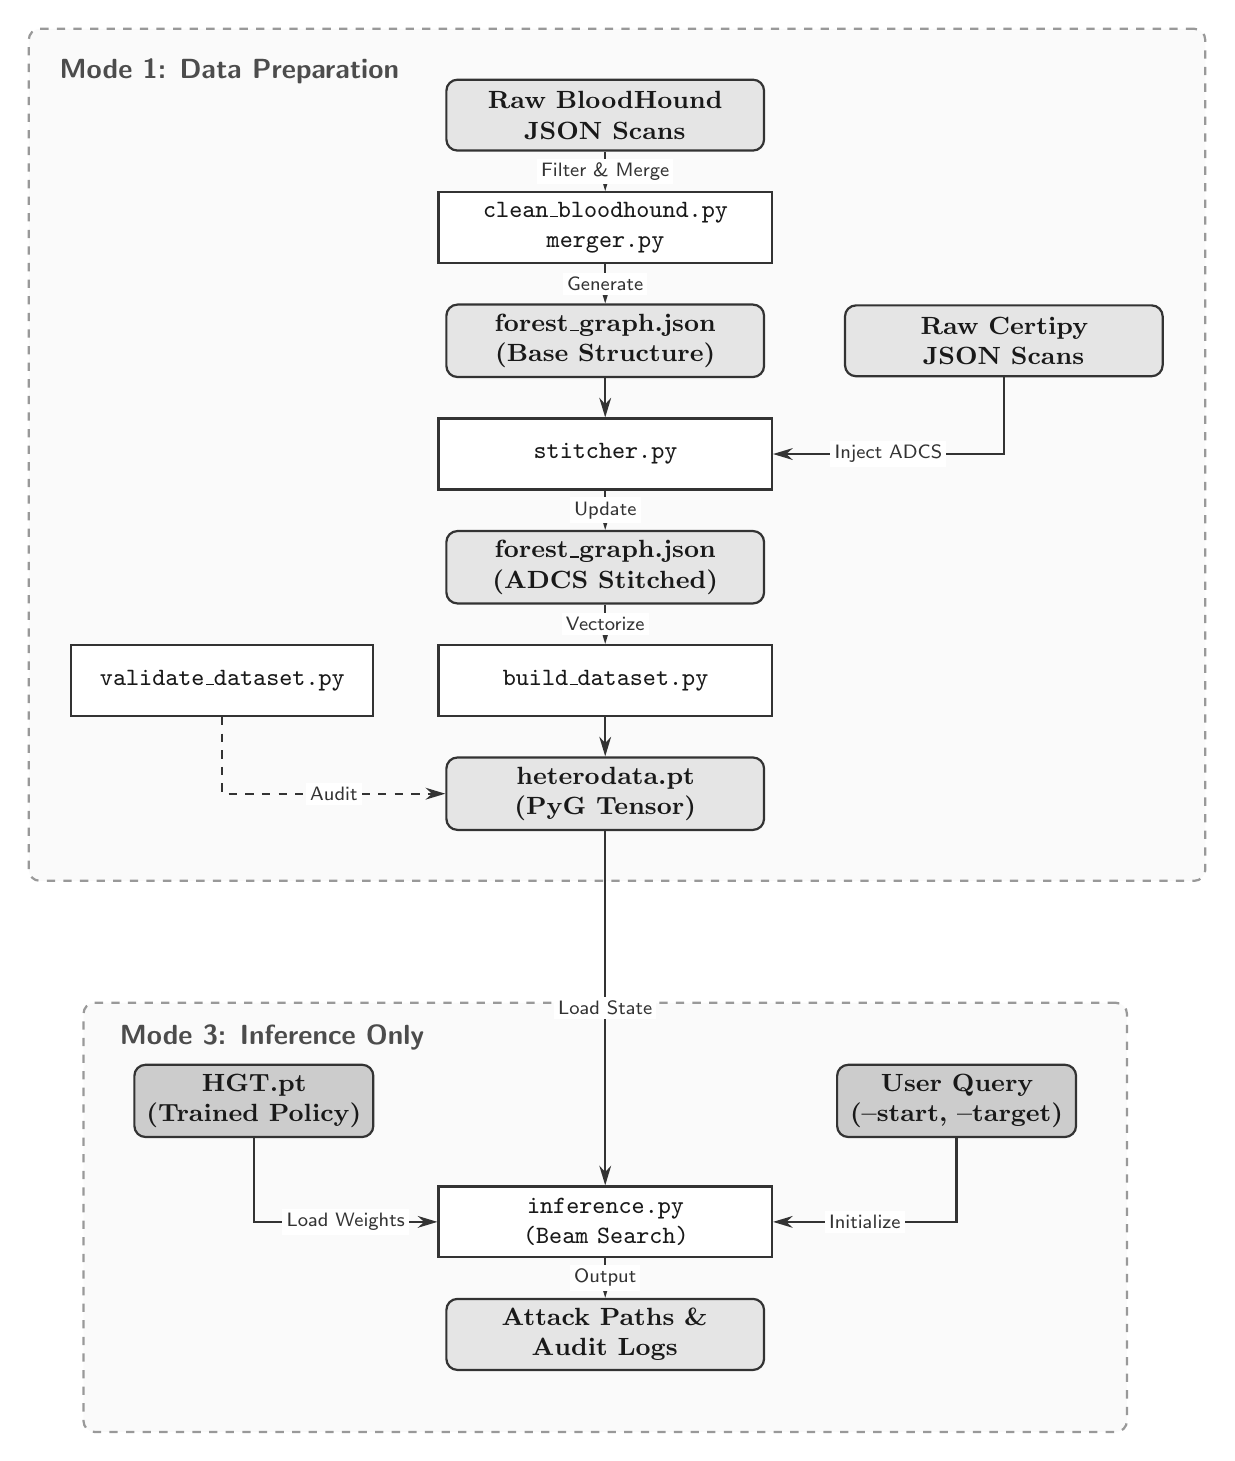
\begin{tikzpicture}[
        % Tighter node distances for a compact vertical footprint
        node distance=0.5cm and 0.8cm,
        % Data artifacts: Light gray fill, dark border, rounded
        data/.style = {rectangle, draw=black!80, fill=black!10, thick, rounded corners, 
                       text width=3.8cm, align=center, minimum height=0.9cm, 
                       font=\small\bfseries\color{black!90}},
        % Scripts: White fill, dark border, sharp corners
        script/.style = {rectangle, draw=black!80, fill=white, thick, 
                         text width=4cm, align=center, minimum height=0.9cm, 
                         font=\small\ttfamily\color{black!90}},
        % External inputs/models: Medium gray fill, dark border, rounded
        external/.style = {rectangle, draw=black!80, fill=black!20, thick, rounded corners, 
                           text width=2.8cm, align=center, minimum height=0.9cm, 
                           font=\small\bfseries\color{black!90}},
        % Arrows: Dark gray/black
        arrow/.style = {draw, thick, -{Stealth[length=2.5mm, width=1.5mm]}, color=black!80},
        dashed_arrow/.style = {draw, thick, dashed, -{Stealth[length=2.5mm, width=1.5mm]}, color=black!80},
        % Edge labels: placed automatically at the 75% mark
        edge_lbl/.style = {font=\scriptsize\sffamily, color=black!80, align=center, fill=white, inner sep=1.5pt}
    ]

    % --- Row 1 & 2: Initial BloodHound Flow ---
    \node[data] (bh_raw) {Raw BloodHound\\JSON Scans};
    \node[script, below=of bh_raw] (merger) {clean\_bloodhound.py\\merger.py};
    \node[data, below=of merger] (base_graph) {forest\_graph.json\\(Base Structure)};

    % --- Row 3: Stitching (Certipy enters laterally) ---
    \node[script, below=of base_graph] (stitcher) {stitcher.py};
    \node[data, right=1.0cm of base_graph] (certipy) {Raw Certipy\\JSON Scans};

    % --- Row 4 & 5: Final Graph & Builder ---
    \node[data, below=of stitcher] (stitched_graph) {forest\_graph.json\\(ADCS Stitched)};
    \node[script, below=of stitched_graph] (builder) {build\_dataset.py};
    
    % --- Row 6: Tensor (Validator enters laterally) ---
    \node[script, left=0.8cm of builder, text width=3.6cm] (validator) {validate\_dataset.py};
    \node[data, below=of builder] (tensor) {heterodata.pt\\(PyG Tensor)};

    % --- Row 7: Inference Phase ---
    % FIX: Increased drop from 2.2cm to 3.5cm to stop the boxes from colliding!
    \node[script, below=4.5cm of tensor] (inference) {inference.py\\(Beam Search)};
    \node[external, above left=0.6cm and 0.8cm of inference] (model) {HGT.pt\\(Trained Policy)};
    \node[external, above right=0.6cm and 0.8cm of inference] (query) {User Query\\(--start, --target)};

    % --- Row 8: Output ---
    \node[data, below=of inference] (output) {Attack Paths \&\\Audit Logs};

    % --- Edges (Arrows) ---
    % Prep Flow
    \draw[arrow] (bh_raw) -- node[edge_lbl] {Filter \& Merge} (merger);
    \draw[arrow] (merger) -- node[edge_lbl] {Generate} (base_graph);
    \draw[arrow] (base_graph) -- (stitcher);
    \draw[arrow] (stitcher) -- node[edge_lbl] {Update} (stitched_graph);
    \draw[arrow] (stitched_graph) -- node[edge_lbl] {Vectorize} (builder);
    \draw[arrow] (builder) -- (tensor);
    
    % Lateral "Down and Bend" Arrows
    \draw[arrow] (certipy) |- node[edge_lbl, pos=0.75] {Inject ADCS} (stitcher);
    \draw[dashed_arrow] (validator) |- node[edge_lbl, pos=0.75] {Audit} (tensor);
    
    % Inference Flow
    \draw[arrow] (tensor) -- node[edge_lbl] {Load State} (inference);
    \draw[arrow] (model) |- node[edge_lbl, pos=0.75] {Load Weights} (inference);
    \draw[arrow] (query) |- node[edge_lbl, pos=0.75] {Initialize} (inference);
    \draw[arrow] (inference) -- node[edge_lbl] {Output} (output);

    % --- Background Boxes to denote modes ---
    \begin{scope}[on background layer]
        % Data Prep Mode Box
        \node[rectangle, draw=black!40, fill=black!2, dashed, rounded corners, thick, 
              fit=(bh_raw) (certipy) (validator) (tensor), inner xsep=15pt, inner ysep=18pt] (prep_box) {};
        % FIX: Shifted the label down and right so it stops crossing the dashed line
        \node[anchor=north west, font=\sffamily\bfseries\color{black!70}] 
              at ([xshift=8pt, yshift=-8pt]prep_box.north west) {Mode 1: Data Preparation};

        % Inference Mode Box
        \node[rectangle, draw=black!40, fill=black!2, dashed, rounded corners, thick, 
              fit=(model) (query) (inference) (output), inner xsep=18pt, inner ysep=22pt] (inf_box) {};
        % FIX: Shifted the label down and right
        \node[anchor=north west, font=\sffamily\bfseries\color{black!70}] 
              at ([xshift=10pt, yshift=-5pt]inf_box.north west) {Mode 3: Inference Only};
    \end{scope}

    \end{tikzpicture}
    \caption{Data Pipeline flow.}
    \label{fig:pipeline_architecture}
\end{figure}

\subsection{\texttt{clean\_bloodhound.py}: Filtering and Multi-Domain Accumulation}
\label{sec:clean_bloodhound}

The initial stage of the data preparation pipeline is handled by the 
\texttt{clean\_bloodhound.py} script, which is responsible for sanitizing 
raw BloodHound JSON outputs. To support 
large-scale enterprise environments, the script implements a recursive, 
multi-domain accumulation mechanism. This ensures that when input 
data contains scans from multiple domains or is split across various 
files, no topological data is silently overwritten. The script 
accomplishes this by deduplicating entities based on their 
\texttt{ObjectIdentifier} (\gls{sid}), selectively retaining the ``richer'' 
JSON record if duplicate scans of the same domain occur.

Crucially, this component acts as a noise-reduction filter to optimize 
the \gls{gnn}'s computational overhead. It builds an initial edge 
index across all entities to determine topological connectedness. 
Using this index, the script systematically drops 
irrelevant nodes. For example, \texttt{Computer} nodes matching 
standard workstation naming conventions (e.g., \texttt{WKS-0}) are pruned 
if they lack dangerous \gls{acl} privileges, unconstrained delegation 
rights, and possess an edge degree of one or less. Similarly, 
disabled \texttt{User} nodes are purged from the dataset unless they 
retain active sessions or explicit \gls{acl} edges, while empty 
\texttt{Group} objects with no members or outbound privileges are entirely 
discarded. Nodes representing Domains, \glspl{gpo}, and \glspl{ou} 
are preserved as-is to maintain structural hierarchy.

\subsection{\texttt{merger.py}: Normalisation and Merging}
\label{sec:merger}

Following the initial filtering and \gls{adcs} data stitching, the 
pipeline executes \texttt{merger.py}. This script functions as a 
generic forest merger, capable of accepting heterogeneous inputs such as 
directories of cleaned JSON files or previously stitched domain graphs and 
consolidating them into a unified \texttt{forest\_graph.json} structure. Positioned directly before the tensor construction phase, this 
module is strictly responsible for cryptographic and structural alignment.

To ensure flawless tensor mapping in PyTorch Geometric, the script 
enforces a strict normalization protocol. All 
\texttt{ObjectIdentifier} and \texttt{PrincipalSID} values, including 
cross-domain \texttt{TargetDomainSid} references, are strictly cast to 
uppercase, while key categorical properties (such as \texttt{name}, 
\texttt{domain}, and \texttt{RightName}) are normalized to lowercase. 

When merging overlapping datasets, the script resolves conflicts through 
a deterministic scoring heuristic. The \texttt{score\_obj} function 
evaluates node richness by awarding points for populated properties, 
active \gls{acl} rules, and group members, while applying a heavy 
multiplier to explicit cross-domain \texttt{Trusts} . The 
conflicting entity with the highest topological score is retained. 
Finally, the script executes a validation routine that inventories all 
discovered trust relationships, aggregates edge type frequencies, and 
calculates a ``dangling-reference rate'' to quantify relational 
integrity before the data is vectorized into the \gls{gnn}.

\subsection{\tool{stitcher.py}: ADCS Injection and Domain Detection}
\label{sec:stitcher}

Because Certipy operates independently of BloodHound, its raw JSON output 
lacks the native topological bindings required to merge seamlessly into an 
existing \gls{ad} graph. To bridge this gap, the pipeline employs 
\tool{stitcher.py}, an intermediate augmentation script positioned directly 
between the filtering and merging phases. Before the script is 
even invoked, the pipeline's overarching wrapper automatically parses the 
Certipy output to dynamically detect the target domain. By analyzing 
the Certificate Subject or Distinguished Name embedded within the 
scanned certificates, the wrapper extracts the domain context and passes it to the stitcher without requiring manual operator input.

Once invoked, the script injects two novel node categories into the graph: 
\gls{ca} and \texttt{certtemplates}. 
Because Certipy does not natively retrieve \glspl{sid} for these entities, 
the script generates deterministic, synthetic Ghost \glspl{sid} (e.g., 
\texttt{S-1-5-21-GHOST-...}) by computing an MD5 hash of the template name 
and the target domain. To connect these isolated nodes to the 
broader network, the script builds a resolution dictionary that maps 
lowercase principal names to their existing \texttt{ObjectIdentifier} 
within the forest. It then translates complex \gls{adcs} 
relationships into standard BloodHound \texttt{Aces} entries, injecting 
edges such as \edge{Enroll}, \edge{PublishedTo}, and \edge{WriteDACL}. 
Critically, it also injects an \edge{HttpEnroll} edge to model ESC8 
vulnerabilities, and a \edge{TrustedForNTAuth} edge to link the \gls{ca} 
back to the domain root, preventing the routing algorithm from dead-ending.

Beyond explicit \gls{adcs} integration, \tool{stitcher.py} acts as the 
engine for synthetic \gls{apt} vector generation. It proactively 
scans the forest for logically vulnerable delegation configurations. 
If a source entity possesses \texttt{unconstraineddelegation} rights, the 
script dynamically generates a \edge{coercetgt} edge to mathematically 
represent \gls{ntlm} coercion attacks (e.g., PetitPotam). To 
preserve topological integrity, this script strictly validates that the 
target is an unprotected Domain Controller computer account, strictly 
preventing the \gls{gnn} from calculating illogical attack paths through 
abstract entities like \glspl{ou} or standard user accounts.



\subsection{Training Environment: GOAD}
% Game of Active Directory: ~3 domains, deliberately vulnerable AD lab.
% Used exclusively for training.
% 33 traces define the coverage ceiling of the model.

The Game of Active Directory (GOAD), developed by Mayfly, serves as the primary 
training and diagnostic environment for this research. GOAD is a highly complex, 
multi-domain, and multi-forest vulnerable lab designed specifically to simulate 
advanced, real-world enterprise architectures. The environment is composed of five 
virtualized Windows Server machines running Windows Server 2016 and 2019 
distributed across two distinct forests. The primary forest contains a parent 
domain \texttt{sevenkingdoms.local} and a child domain 
\texttt{north.sevenkingdoms.local}, simulating a typical corporate hierarchy 
with bidirectional transitive trusts. A secondary, external forest 
\texttt{essos.local} is connected via a forest-to-forest trust with SID history 
enabled. This sophisticated topological layout provides the heterogeneous graph 
structure required to train the Graph Neural Network on cross-domain lateral 
movement and complex trust exploitations.

\begin{figure}[h]
    \centering
    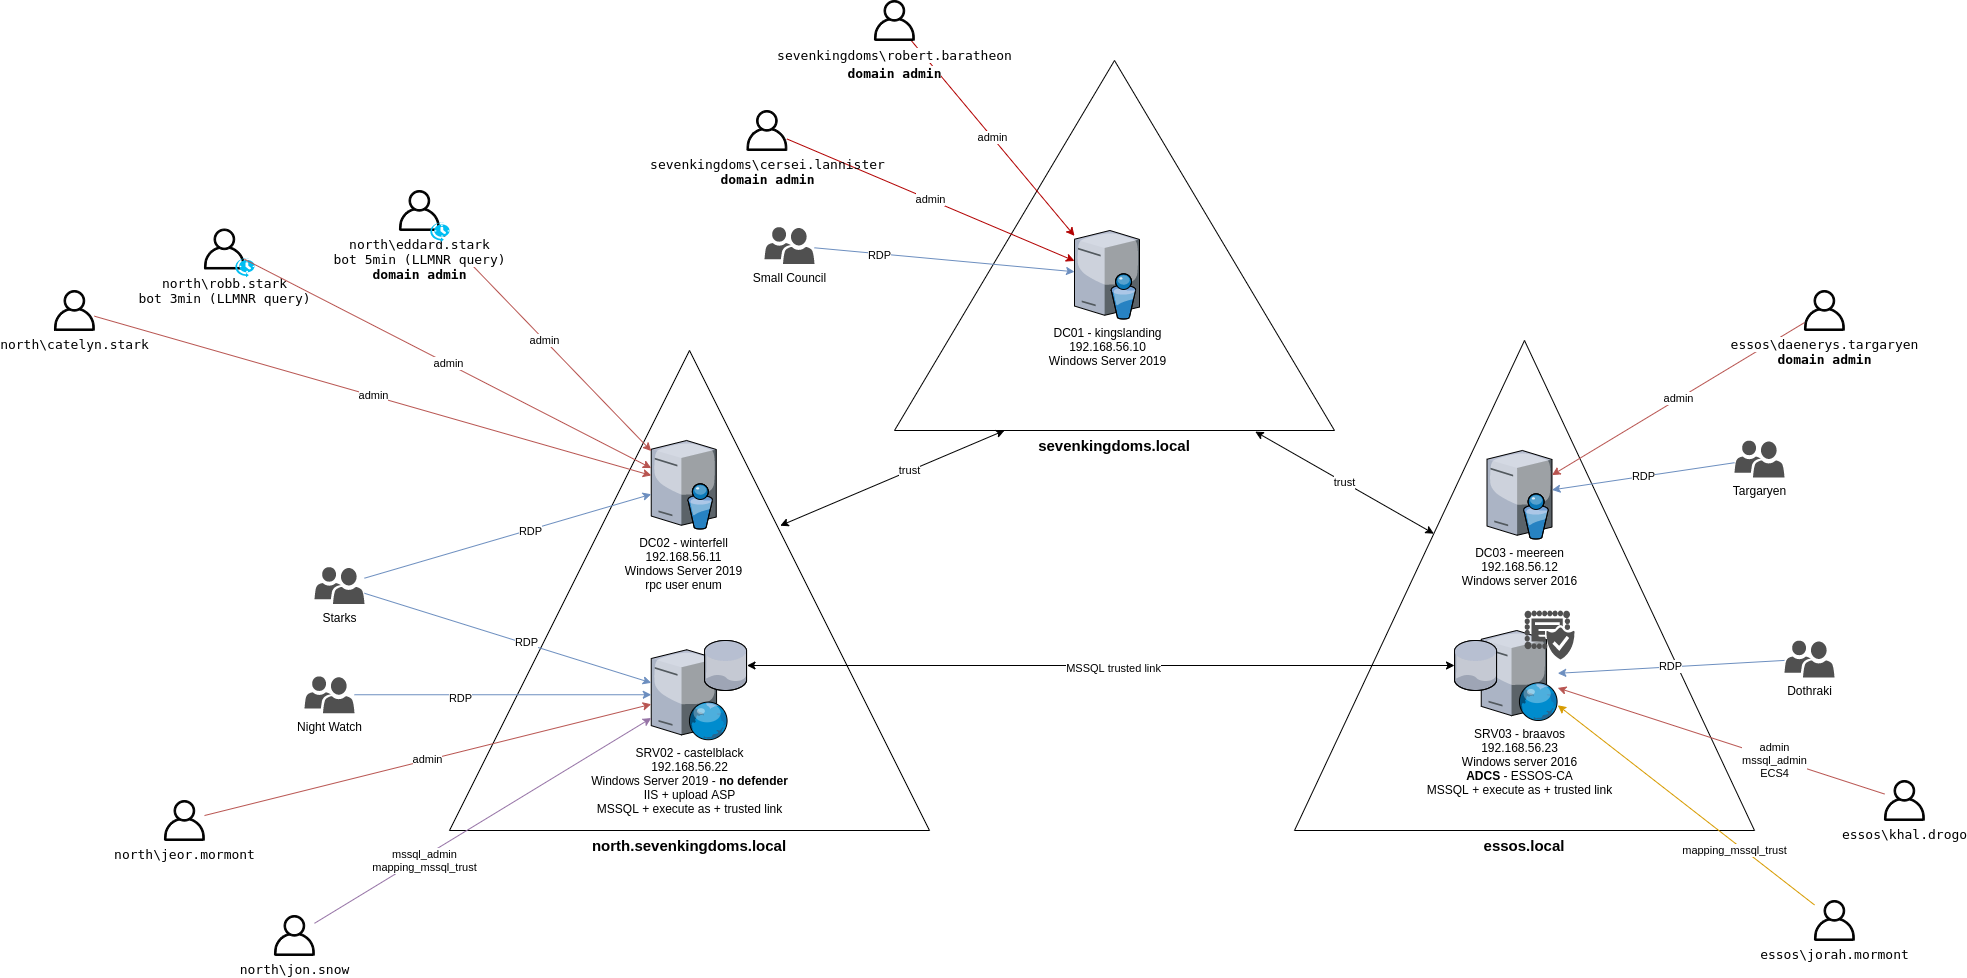
\includegraphics[width=0.85\textwidth]{ressources/goad_overview.png}
    \caption{The logical architecture and domain topology of the GOADv2 
    environment. \textit{Source: Mayfly (2022)}.}
    \label{fig:goad_architecture}
\end{figure}

Beyond basic network topography, GOAD is engineered with deeply embedded, 
configuration-level vulnerabilities that test the limits of automated attack 
path discovery. The environment features multi-step \gls{acl} 
kill-chains, deliberately exposed \gls{adcs} 
configured to be vulnerable to ESC1 through ESC3 and ESC8 relay attacks, and 
various forms of delegation (Unconstrained, Constrained, and Resource-Based 
Constrained Delegation). By exposing the Navigation Model to this dense 
concentration of intersecting vulnerabilities, the network learns to evaluate 
competing escalation routes—such as choosing between a force change password 
against an IIS server or a stealthy \texttt{WriteDACL} abuse—making GOAD an 
ideal foundational dataset for imitation learning in offensive security.
The attack paths goad provides are to be presented in a learnable and readable training format for the model. Each attack path is deconstructed into transitions,
 \texttt{current\_node}, \texttt{next\_hope}, \texttt{credentials\_used}, 
 \texttt{total}, \texttt{path\_weight}, \texttt{train\_on\_step}, \texttt{notes} 
and the \texttt{step\_cost}.


\subsection{Feature engineering}

To a GNN model learning from a bloodhound scan, attack paths are of different importance, 
some are totaly invisible while others are a gold mine for what the model needs to replicate.
Paths that rely on unpatched vulnerabilities or outdated systems, for instance, leave no trace in the 
BloodHound graph and are marked with a \texttt{path\_weight} of 0.
Paths that are mostely visible with only two or less transitions that do not qualify have the latter marked
through \texttt{train\_on\_step} set to zero.
And at last, for an imitation learning model, given the choice between two valide transitions, the model
choses based on training data, prefering the edge type it has seen most during training. To address this
We are to more or less guide  the model to gravitate towards the edge attack with less impact on 
the environment, the one with less noise and impact. To reach the desired effect each valid transition
is scored. This score is reflected directly in the loss function through the \texttt{step\_cost} feature.

\begin{table}[H]
\centering
\caption{Step cost assignment by attack category.}
\label{tab:step_cost}
\begin{tabularx}{\textwidth}{>{\bfseries}l c X}
\toprule
Attack Category & Cost Range & Rationale \\
\midrule
Topological / Logical  & 0.1 -- 0.2 &
  Operations such as adding a member to a group or enrolling in a 
  certificate template. These transitions are structurally clean and 
  rarely trigger alerts unless heavy auditing is configured. \\[6pt]

Credential Abuse & 0.3 -- 0.4 &
  Using a recovered password or a forged TGT. Low noise overall, 
  but detectable by honeytokens or behavioural analysis tools. \\[6pt]

Active Enumeration & 0.5 &
  Kerberoasting or intensive LDAP queries. Intermediate noise level; 
  commonly detected by modern SIEMs monitoring ticket requests or 
  query volume anomalies. \\[6pt]

Memory / Disk Dumping & 0.6 -- 0.7 &
  Dumping the SAM database or LSASS process memory. High detection 
  risk; endpoint protection tools such as Microsoft Defender and 
  CrowdStrike flag these operations near-immediately. \\[6pt]

Network Exploitation & 0.8 -- 0.9 &
  Active coercion and relay attacks such as PetitPotam or NTLM 
  Relaying, and brute-force techniques such as password spraying. 
  Very noisy; triggers IDS/IPS rules and account lockout policies. \\
\bottomrule
\end{tabularx}
\end{table}

The \texttt{step\_cost} value assigned to each transition feeds 
directly into the loss function through the effective weight 
computation:


The feature engineering phase introduced three mechanisms: 
filters to eliminate CVE-dependent transitions invisible to the graph 
collector; path weights reflecting a composite visibility score that 
prioritises transitions where the graph structure itself is the primary 
escalation vector; and a \texttt{step\_cost} feature guiding the model 
toward stealthier, less impactful edges when a choice presents itself. 
This constitutes a simplified reward shaping approach, consistent with 
standard practices in the imitation learning literature.


% ─────────────────────────────────────────────────────────────

\section{Navigation Model}

\subsection{HGT Encoder}

To effectively process the highly asymmetrical and heterogeneous structure
of \gls{ad}---which contains distinct entity types (e.g., users, computers,
groups, domains) alongside a complex vocabulary of privilege edges---the
architecture utilises an \gls{hgt} encoder \cite{hu2020heterogeneous}. 
Implemented via the \gls{pyg} library, the encoder is specifically designed 
to handle the native topological variations without requiring manual 
modification of the graph, preserving the distinct semantic meaning of 
each node and edge type as established in the foundational \gls{hgt} 
literature.

The encoding phase begins by projecting the disparate input features of
each node type into a unified dimensional space. This is achieved by 
passing the raw features through type-specific linear projection networks, 
mapping every object into a standardised 64-dimensional hidden vector. 
Once projected, the architecture applies a series of \gls{hgt} convolutional layers 
utilising multi-head attention mechanisms to propagate context across the 
network. Specifically, the model employs four attention heads across two 
sequential message-passing layers. This bounded depth prevents the 
over-smoothing of node features while still allowing the network to aggregate 
vital context from a node's local topology. 

Through this mechanism, the encoder intrinsically learns the semantic
value of various edge types---for example, mathematically distinguishing
between a standard \texttt{GenericWrite} and a high-privilege
\texttt{MemberOf} relationship. The final output of the encoder is a dense, 
concatenated embedding matrix where every object in the \gls{ad} network is 
represented as a sophisticated 64-dimensional vector that encapsulates its 
structural privilege and potential attack utility.

\subsection{Policy Head}

Following the extraction of topological features, the navigation model
must evaluate and rank potential escalation paths. This decision-making 
phase is governed by the Policy Head. During traversal, the inference 
algorithm isolates the attacker's current node and identifies all topologically 
valid outbound neighbours. 

To score these candidate transitions, the Policy Head leverages the
embeddings generated by the \gls{hgt} encoder. Rather than computing a 
rigid concatenation of the current state and a fixed target state, the model 
evaluates the transition via the Hadamard product (element-wise multiplication) 
between the current node's expanded embedding and each candidate neighbour's 
embedding. This element-wise interaction matrix is then processed through 
a \gls{mlp} consisting of consecutive linear transformations, \gls{relu}
activations, and dropout layers. 

The \gls{mlp} ultimately compresses this latent relationship into a
single scalar confidence score for each candidate. By relying on the 
relative, multiplicative interaction between node embeddings, the policy head 
acts as a generalised privilege evaluator. It steers the algorithmic 
traversal toward high-value nodes based strictly on the structural context 
learned during the encoding phase, completely decoupling the pathfinding logic 
from hardcoded heuristic rules.

\subsection{Loss Function and Step Cost}

To train the policy head to navigate not just efficiently, but stealthily, 
the architecture employs a weighted cross-entropy loss function. The effective 
training weight for each transition is calculated as follows:

\begin{equation}
  \text{eff\_weight} = \text{path\_weight} \times (1 - \text{step\_cost})
  \label{eq:eff_weight}
\end{equation}

\noindent where \texttt{path\_weight} reflects the overall visibility 
and quality of the full attack path, and \texttt{step\_cost} 
penalises individual transitions according to their noise category 
in Table~\ref{tab:step_cost}. A high \texttt{step\_cost} reduces the 
effective training weight of that transition, making the model less 
likely to replicate it when a lower-cost alternative exists in the 
training data. Conversely, topological transitions with a low 
\texttt{step\_cost} receive a higher effective weight and are 
reinforced more strongly during training. The result is a model that, 
when faced with a choice between two structurally valid transitions, 
gravitates toward the one with less environmental impact --- not 
because it was explicitly told to, but because the training signal 
made that choice more frequent and more rewarded.

This reward shaping mechanism fundamentally alters the pathfinding paradigm 
compared to traditional graph traversal algorithms. Standard shortest-path 
algorithms, such as Dijkstra's algorithm implemented in default BloodHound, 
traverse the network by treating all edges as having an equal weight of one. 
Consequently, they inherently optimise for the shortest structural distance, 
which frequently results in highly detectable, noisy exploit chains. 

By integrating the \texttt{step\_cost} directly into the loss function, the 
neural network is mathematically discouraged from selecting loud transitions 
during the imitation learning phase. Instead of merely memorising the shortest 
routes from the training corpus, the policy head internalises an OPSEC-driven 
heuristic. During inference, this enables the model to discover non-linear, 
multi-hop \gls{lotl} paths that exhibit a significantly 
lower cumulative detectability cost than routes generated by unweighted 
Dijkstra searches on the exact same topology. This capability to prioritise 
stealth over topological proximity forms the core justification for deploying 
deep learning in automated offensive navigation.

% ─────────────────────────────────────────────────────────────
\section{Beam Search Navigation}

\subsection{Beam Search Navigation}

\subsubsection{Algorithm}

The core pathfinding engine during inference is a heuristic beam search 
algorithm designed to evaluate and navigate the topological structures 
extracted by the \gls{hgt} encoder. At each transition step, the 
algorithm queries the policy head to score all valid outbound neighbours, 
converting the raw logits into a probability distribution via a Softmax 
function. Rather than selecting the single best transition, 
the beam search maintains a tracked list of the top $k$ candidate paths 
(the beam width), expanding each and accumulating their transition 
probabilities logarithmically to prevent mathematical underflow.

Crucially, the algorithm includes a fallback mechanism for undocumented or 
\gls{oov} edge types. If the inference engine encounters 
a relationship that the neural network did not observe during training, it 
bypasses the policy head's probabilistic output and assigns a static baseline 
operational score of $0.05$. This ensures the pipeline remains resilient 
and does not crash when deployed against evolving \gls{ad} environments with 
novel schema additions.

\begin{algorithm}[H]
  \DontPrintSemicolon
  \SetAlgoLined
  \KwIn{Graph $G$, Start Node $S$, Target Node $T$, Beam Width $k$, Max Depth $D$}
  \KwOut{Top $k$ Attack Paths}
  $\text{beam} \leftarrow [(\text{score: } 0.0, \text{path: } [S])]$\;
  $\text{completed} \leftarrow []$\;
  \For{$d \leftarrow 1$ \KwTo $D$}{
    $\text{candidates} \leftarrow []$\;
    \ForEach{$(\text{score}, \text{path}) \in \text{beam}$}{
      $C \leftarrow \text{path}[-1]$\;
      \If{$C = T$ \textbf{or} $\text{HasDCSync}(C, T)$}{
        $\text{completed}\text{.append}((\text{score}, \text{path}))$\;
        \textbf{continue}\;
      }
      $\text{neighbours} \leftarrow \text{GetValidNeighbours}(C)$\;
      $\text{probs} \leftarrow \text{PolicyHead}(C, \text{neighbours})$\;
      \ForEach{$N, \text{prob} \in (\text{neighbours}, \text{probs})$}{
        \If{$\text{IsOOVEdge}(C, N)$}{
          $\text{prob} \leftarrow 0.05$\;
        }
        $\text{new\_score} \leftarrow \text{score} + \log(\text{prob})$\;
        $\text{candidates}\text{.append}((\text{new\_score}, \text{path} + [N]))$\;
      }
    }
    $\text{beam} \leftarrow \text{TopK}(\text{candidates}, k)$\;
    \If{$\text{length}(\text{completed}) \geq k$}{
      \textbf{break}\;
    }
  }
  \Return $\text{TopK}(\text{completed} \cup \text{beam}, k)$\;
  \caption{Heuristic Beam Search for Attack Path Discovery}
  \label{algo:beam_search}
\end{algorithm}


\subsubsection{Terminal State: \gls{dcsync}}

To optimise traversal and mimic the operational objectives of a professional 
red team, the inference engine employs a dynamic, state-aware termination 
condition rather than blindly searching for an exact target node match. 
At each step, the algorithm evaluates whether the current node possesses 
\gls{dcsync} privileges over the target's domain. Specifically, it 
checks for the combination of \texttt{GetChanges}, \texttt{GetChangesAll}, and 
\texttt{GetChangesInFilteredSet} directory replication rights. 

If a path reaches a node holding these privileges, the algorithm recognises 
global reachability and immediately halts, trimming any subsequent expansion 
. This assumes total domain compromise, acknowledging that an attacker 
with \gls{dcsync} rights can organically forge the remaining transitions to reach 
the final objective without requiring further algorithmic guidance.


\subsubsection{Cross-Environment Inference and Global Coordinate System}

A critical engineering challenge during deployment is bridging the gap between 
the strictly heterogeneous data structures required by the neural network and 
the homogeneous, indexed lookups required by classical search algorithms. 

During the initial ingestion and encoding phase, the graph strictly maintains 
its heterogeneity. The \gls{hgt} processes the environment using isolated 
feature dictionaries and type-specific edge indices, ensuring the message 
passing mathematically preserves the distinct semantic nature of users, 
computers, and disparate \gls{ad} permissions.

However, once the latent embeddings are extracted, tracking complex 
multidimensional tuples (e.g., \texttt{('computers', 12)}) during a rapid, 
multi-hop heuristic beam search introduces severe computational overhead. To 
resolve this, the inference module dynamically constructs a unified global 
coordinate system post-encoding. 

The heterogeneous embeddings are concatenated into a singular, flattened 
tensor space, and all structural edges are mathematically shifted using 
pre-calculated type offsets. This creates a global adjacency mapping for the 
deterministic search algorithm. It allows the beam search to execute highly 
efficient integer-based traversals (e.g., jumping from global Node 15 to Node 
102) while still querying the policy head with the rich, heterogeneously 
derived latent vectors. This dynamic ingestion and coordinate resolution allow 
the model to execute inferences on completely unseen, enterprise-scale forests 
without requiring any structural modifications to the base \gls{hgt}.


\subsection{Audit Module}

Because deep learning models operate probabilistically, the pipeline includes 
a deterministic audit module to evaluate the semantic quality and operational 
viability of the generated attack paths. The module categorises outputs 
into three distinct reliability tiers:

\begin{itemize}
    \item \textbf{Ok:} The path successfully reaches the explicit target 
    node or terminates at a node possessing direct \gls{dcsync} privileges 
    over the target domain, signifying a complete operational success.
    \item \textbf{Warn:} The path identifies a critical escalation route 
    but requires human improvisation to complete. For example, this 
    occurs if the model achieves \gls{dcsync} on a foreign domain, necessitating 
    a cross-forest SID History attack, or if the beam search terminates 
    structurally with noisy edges such as \texttt{MemberOf} or \texttt{Contains} 
    without reaching the final target.
    \item \textbf{Fail:} The path represents an operational dead-end. 
    This is triggered if the beam search is unable to progress past the 
    starting node or terminates at an unprivileged object lacking domain 
    replication rights.
\end{itemize}

By pairing neural pathfinding with this strict heuristic audit, the tool 
ensures operators receive transparent, actionable intelligence alongside 
clear diagnostics when the algorithmic routing falls short.

\section{Validation Module \& Logging}

To ensure operational transparency and deterministic execution, the 
architecture implements a centralised logging framework that captures both 
standard output and error streams across all pipeline stages. From the 
initial heterogeneous data ingestion to the final algorithmic traversal, 
every data mutation, structural shift, and inference decision is immutably 
recorded. By multiplexing the execution stream---providing operators with 
real-time diagnostic feedback while simultaneously committing telemetry to a 
persistent log---the system guarantees a comprehensive historical audit 
trail for subsequent evaluation or architectural debugging.

Prior to initiating the neural network or training phases, a dedicated 
validation module systematically audits the extracted graph tensors and 
the supervised training corpus against a strict set of expected baselines. 
It evaluates the mathematical health of the embeddings, confirms the 
preservation of critical operational pathways (such as \gls{adcs} escalation 
routes), and eliminates topological anomalies like self-loops. Crucially, 
it cross-references the expected outcomes---the documented target hops within 
the training examples---against the constructed graph to ensure all objective 
coordinates accurately map to valid boundaries within the heterogeneous 
tensors. By classifying structural deviations as either informational warnings 
or fatal execution blockers, the module guarantees that only mathematically 
sound and topologically viable data reaches the \gls{hgt} encoder.

%% ============================================================
%%  CHAPTER 3 — IMPLEMENTATION
%% ============================================================
\chapter{Implementation}

\section{Technical Stack}

The \texttt{GNN-AD-Navigator} pipeline is engineered entirely in Python, 
leveraging an ecosystem of specialised libraries for deep learning, graph 
processing, and interactive visualisation. The core neural network 
architecture and heterogeneous tensor operations are implemented using 
\texttt{PyTorch} and \texttt{PyTorch Geometric (PyG)}. For graph topology 
manipulation and deterministic traversal algorithms (such as the heuristic 
beam search), the system relies heavily on \texttt{NetworkX}.

To provide operators with an accessible and interactive frontend, the audit 
module and visualisations are built using \texttt{Streamlit}, coupled with 
\texttt{Pyvis} for dynamic, browser-based rendering of the discovered 
attack paths. 

Model training was offloaded to cloud-based Kaggle compute instances to 
manage the heavy matrix multiplications required by the Heterogeneous Graph 
Transformer. Specifically, the training pipeline was pinned to dual NVIDIA 
Tesla T4 \glspl{gpu}. This specific hardware selection was a deliberate 
engineering constraint; older architectures like the Tesla P100 (which 
utilise the \texttt{sm\_60} compute capability) exhibit architectural 
incompatibilities with the compiled CUDA binaries of modern \texttt{PyTorch} 
releases. 

To ensure strict reproducibility across environments, the core dependencies 
were version-pinned as detailed in Table~\ref{tab:tech_stack}.

\begin{table}[h]
    \centering
    \renewcommand{\arraystretch}{1.2}
    \begin{tabular}{@{}ll@{}}
        \toprule
        \textbf{Library / Framework} & \textbf{Version} \\ 
        \midrule
        Python & 3.10.x \\
        PyTorch & 2.1.0+cu118 \\
        PyTorch Geometric (PyG) & 2.4.0 \\
        NetworkX & 3.1 \\
        Streamlit & 1.28.0 \\
        Pyvis & 0.3.2 \\
        \bottomrule
    \end{tabular}
    \caption{Core technical stack and version pinning for 
    environment reproducibility.}
    \label{tab:tech_stack}
\end{table}


\section{Repository Structure}

The project repository is organised into a highly modular, pipeline-driven 
architecture. This separation of concerns ensures that data ingestion, 
neural network training, and frontend visualisation remain strictly decoupled. 
The directory tree is structured as follows:

\begin{verbatim}
gnn-ad-navigator/
├── examples/           # Sample AD graphs and expected pipeline outputs
├── gui/                # Streamlit frontend (app.py, visualisation.py)
├── lib/                # Core modules and helper functions
├── models/             # Serialised PyTorch weights (.pt checkpoints)
├── notebooks/          # Jupyter/Kaggle notebooks for model training
├── scripts/            # Core pipeline execution scripts
│   ├── build_dataset.py
│   ├── clean_bloodhound.py
│   ├── inference.py
│   ├── merger.py
│   ├── prepare_training_examples.py
│   ├── stitcher.py
│   └── validate_dataset.py
├── thesis/             # LaTeX source code for the manuscript
├── .dockerfile         # Containerised deployment configuration
├── .gitignore          # Strict ignore rules for sensitive data
├── launch.sh           # Master bash script for pipeline execution
├── README.md           # Documentation and setup instructions
├── requirements.txt    # Python dependencies
└── setup.sh            # Environment initialisation script
\end{verbatim}

A critical security consideration within the repository's configuration is 
the \texttt{.gitignore} file. Given the highly sensitive nature of 
Active Directory environments, the repository enforces strict exclusion 
paranoia. All \texttt{.json} scans, \texttt{Certipy} outputs, and compiled 
\texttt{.pt} tensors are explicitly ignored by version control to ensure 
that no real-world or client-specific infrastructure data is ever 
inadvertently committed to the public history, The only exception being
the included test environment INLANEFREIGHT.local scans.

% ─────────────────────────────────────────────────────────────
\subsection{Script Responsibilities and Data Flow}

To maintain strict modularity and ensure reproducibility across disparate 
environments, the execution of the data pipeline is fully decoupled from 
the underlying Python scripts. The entire lifecycle---from raw data 
ingestion to algorithmic inference---is managed by a master shell 
orchestrator (\texttt{launch.sh}). 

This orchestrator sequentially routes data through a series of specialised 
Python micro-scripts, handling standard output logging, error trapping, 
and dependency validation between stages. It bifurcates the system into 
two distinct operational modes: a \textit{Data Preparation} phase, which 
compiles the heterogeneous tensors, and an \textit{Inference} phase, which 
executes the heuristic beam search. 

The precise data flow, detailing the structural transformation of 
information at each discrete stage of the pipeline, is outlined in 
Table~\ref{tab:data_flow}.

\begin{table}[h]
    \centering
    \renewcommand{\arraystretch}{1.3}
    \resizebox{\textwidth}{!}{%
    \begin{tabular}{@{}llll@{}}
        \toprule
        \textbf{Stage} & \textbf{Script} & \textbf{Primary Input} & \textbf{Output Artifact} \\ 
        \midrule
        1. Filter & \texttt{clean\_bloodhound.py} & Raw BloodHound \texttt{.json} & Cleaned BloodHound \texttt{.json} \\
        2. Merge & \texttt{merger.py} & Cleaned BloodHound \texttt{.json} & \texttt{forest\_graph.json} (Base) \\
        3. Stitch & \texttt{stitcher.py} & Base Graph + Certipy \texttt{.json} & \texttt{forest\_graph.json} (\gls{adcs} Stitched) \\
        4. Vectorise & \texttt{build\_dataset.py} & Stitched \texttt{forest\_graph.json} & \texttt{heterodata.pt} (PyG Tensor) \\
        5. Audit & \texttt{validate\_dataset.py} & \texttt{heterodata.pt} & Telemetry \& Validation Logs \\
        \midrule
        6. Inference & \texttt{inference.py} & \texttt{heterodata.pt} + User Query & Attack Paths \& Audit Logs \\
        \bottomrule
    \end{tabular}%
    }
    \caption{Sequential data flow and script responsibilities within the GNN-AD-Navigator pipeline.}
    \label{tab:data_flow}
\end{table}

By strictly isolating responsibilities, the pipeline ensures that if 
environmental collection tools (such as BloodHound or Certipy) alter 
their output schemas in the future, only the initial filtering and 
stitching scripts require modification, leaving the core mathematical 
vectorisation and inference engines completely untouched.

\subsection{SharpHound Version Normalisation}

A known architectural fragility within the data ingestion pipeline stems from 
the evolutionary nature of third-party enumeration tools. As collectors like 
SharpHound and \texttt{bloodhound-python} receive updates, their underlying 
\texttt{json} output schemas frequently change. Most notably, the nomenclature 
used to define specific privilege edges is prone to version drift. 

Because the Heterogeneous Graph Transformer (\gls{hgt}) and the underlying 
\gls{pyg} framework require a strictly defined, static edge vocabulary 
during tensor initialisation, encountering an undocumented or altered edge 
string during ingestion will either crash the vectorisation process or cause 
the pipeline to silently drop critical topological data.

To mitigate this schema volatility, the data pipeline implements two explicit 
normalisation strategies prior to tensor construction:

\begin{itemize}
    \item \textbf{Casing Normalisation:} Edge types frequently fluctuate 
    between camel-case and upper-case representations across different tool 
    versions (e.g., \texttt{WriteDACL} versus \texttt{WriteDacl}). The 
    \texttt{merger.py} script resolves this by enforcing aggressive, 
    graph-wide lowercase normalisation on all relationship strings during 
    the initial graph synthesis.
    \item \textbf{Semantic Aliasing:} Tool updates occasionally deprecate 
    entire relationship names in favour of new terminology. For example, 
    legacy trusts represented as \texttt{TrustedBy} must mathematically map 
    to the modern \texttt{SameForestTrust} tensor to ensure the neural 
    network recognises the transition. The \texttt{build\_dataset.py} script 
    implements a static aliasing dictionary to intercept and translate these 
    known schema variations.
\end{itemize}

These interventions are documented as known environmental fragilities rather 
than software bugs. They underscore the necessity of the pipeline's modular 
design, ensuring that string-level normalisation is handled exclusively at 
the data preparation layer so the core mathematical vectorisation engine 
remains isolated from third-party schema drift.

% ─────────────────────────────────────────────────────────────
\section{Training}

\subsection{Training Data: GOAD}

As established in the theoretical framework, the \gls{goad} (Game of Active 
Directory) laboratory serves as the foundational, multi-domain environment 
for this research. To generate the supervised training corpus, a series of 
deterministic attack paths were manually executed within this environment 
and transcribed into a structured trace file.

While the raw trace logs contain nearly 50 discrete execution steps, the 
dataset was rigorously filtered to isolate purely topological transitions. 
Steps requiring out-of-band execution (such as dropping web shells or 
exploiting ghost steps) were pruned, resulting in a refined subset of 
approximately 33 learnable, structurally valid edges. These curated 
transitions were subsequently processed into 52 distinct training examples 
(comprising 26 constrained and 26 unconstrained permutations) to populate 
the PyTorch Geometric \texttt{HeteroData} tensor.

To ensure the policy head develops both precise routing capabilities and 
generalised escalation heuristics, these examples are split into a 
dual-mode training structure:

\begin{itemize}
    \item \textbf{Constrained Examples:} The transition traces provide the 
    model with both an explicit starting node and a predefined target 
    destination. This teaches the network how to mathematically route an 
    attack chain toward a specific coordinate within the graph.
    \item \textbf{Unconstrained Examples:} The traces provide a starting 
    point, but the target is replaced with a \texttt{<null>} sentinel node. 
    This simulates open-ended exploratory escalation, training the model to 
    intrinsically recognise universally high-value targets (such as Tier-0 
    groups or Certificate Authorities) even when an explicit operational 
    objective is not provided.
\end{itemize}

The primary objective of these traces is to teach the \gls{hgt} encoder the 
latent semantic hierarchy of native \gls{ad} permissions. The training 
corpus heavily emphasises \gls{acl} exploitation chains (e.g., 
\texttt{GenericAll}, \texttt{WriteDacl}), nested group inheritance via 
\texttt{MemberOf}, and cross-domain trust transversals, consistently guiding 
the model toward the \gls{dcsync} terminal state.

Crucially, this curated dataset establishes a strict coverage ceiling for 
the model's operational awareness. The training traces deliberately exclude 
transitions reliant on underlying host vulnerabilities, meaning the policy 
head remains blind to \glspl{cve} such as PrintNightmare or ZeroLogon. 
Furthermore, owing to the baseline scope of this specific corpus, advanced 
modern primitives---such as \gls{rbcd} (Resource-Based Constrained 
Delegation), Kerberoasting, and Shadow Credentials---are absent from the 
learnable tensor transitions. This boundary is explicitly acknowledged: the 
neural network cannot reliably infer or prioritise attack vectors that fall 
completely outside its supervised training vocabulary.

\subsection{Kaggle Training Notebook}

The neural network training was executed via a structured Kaggle notebook 
environment to leverage dedicated hardware acceleration. The script 
handles the dynamic ingestion of the \gls{pyg} \texttt{HeteroData} object, 
extracting the discrete arrays of node and edge types to dynamically 
initialise the dimensions of the \gls{hgt} encoder. Following 
instantiation, the notebook executes the training loop over the curated 
constrained and unconstrained permutations, optimising the policy head via 
the custom weighted cross-entropy loss function.

A critical engineering implementation within this notebook resides in the 
model exporting mechanism. Standard PyTorch checkpointing typically 
only saves the raw mathematical weights (the \texttt{state\_dict}). However, 
the training script injects a custom dictionary patch that explicitly bundles 
the graph's structural metadata---specifically the array of node types, edge 
types, the hidden dimension size, and the input feature dimension---directly 
alongside the exported weights. 


\subsection{Model Checkpoints}

The culmination of the training pipeline is the generation of the serialised 
\texttt{HGT.pt} model checkpoint. The metadata patch bundled within 
this file is not merely a logging convenience; it is a strict mathematical 
necessity for conducting cross-environment inference.

Without the bundled metadata, executing inference in a novel \gls{ad} 
environment introduces severe architectural fragility. If a target enterprise 
forest lacks a specific relationship type that was present in the training 
data (or introduces an entirely new, unseen edge), initialising the \gls{hgt} 
dynamically based on the new target graph's schema will result in mismatched 
tensor dimensions. This causes either a hard compiler crash or, far more 
dangerously, a silent architectural misalignment where the trained neural 
weights are shifted and applied to the wrong privilege edges.

\begin{lstlisting}[language=Python, caption={Injecting topological metadata into the PyTorch checkpoint.}, label={lst:metadata_patch}]
# Added metadata and num_features for cross-environment inference
torch.save({
    "epoch":        epoch,
    "model_state":  model.state_dict(),
    "loss":         loss,
    "architecture": "HGT",
    "hidden_dim":   HIDDEN_DIM,
    "num_features": feature_dim,
    "metadata":     metadata
}, CHECKPOINT_HGT)
\end{lstlisting}

By loading the exact structural metadata bundled inside \texttt{HGT.pt}, 
the \texttt{inference.py} script forces the PyTorch engine to reconstruct 
the precise neural architecture present during training. The 
pipeline can then safely project the target environment's data into this 
static schema. Node types present in the model but missing in the target 
environment are safely padded with zero-tensors, and novel edges are bypassed 
using the beam search's out-of-vocabulary fallback logic. This mechanism 
ensures the model's structural integrity remains completely deterministic, 
regardless of the target environment's topological anomalies.

\section{Graphical \& Command Line Interface}

\subsubsection{Operational Context and Future Integrations}

From an architectural standpoint, the \gls{cli} is deliberately positioned 
as the primary execution vector. Professional penetration testers and red 
teamers operate almost exclusively within terminal environments, frequently 
deploying tooling over restricted SSH sessions, pivot proxies, or reverse 
shells. A lightweight, text-based orchestrator integrates seamlessly into 
this operational reality, allowing for automated batch processing and rapid 
retargeting without the overhead of a graphical environment. Conversely, 
the \gls{gui} is provided as a comprehensive supplementary option, designed 
primarily for post-engagement analysis, client reporting, and executive 
presentations where visualising the topological attack chain adds critical 
context.

To further bridge the gap between this automated pathfinding engine and 
established red-team workflows, a highly desirable future integration is 
the native generation of Neo4j Cypher queries. While project time constraints 
prevented its implementation in the current release, future iterations 
could automatically translate the neural network's output into executable 
Cypher syntax. Instead of merely logging a text-based path, the tool would 
generate a structured query instructing the Neo4j backend to explicitly 
match the exact sequence of \glspl{sid} and privilege 
edges identified by the beam search. This would empower operators to copy 
the generated string and instantly project the AI-discovered attack chain 
directly back into their native BloodHound interface for manual validation.

\subsection{CLI}

\subsubsection{Commands and Interactions}

The primary operational interface for the \texttt{GNN-AD-Navigator} is a 
comprehensive command-line orchestrator (\texttt{launch.sh}). Designed with 
efficiency and automation in mind, the \gls{cli} abstracts the underlying 
heterogeneous tensor transformations and Python micro-scripts, presenting the 
operator with a unified, parameterised execution environment.

Rather than forcing the user to manually execute individual scripts in 
sequence, the orchestrator dynamically routes execution based on the provided 
arguments. It structurally supports three distinct operational modes to 
accommodate various phases of a red-team engagement:

\begin{itemize}
    \item \textbf{Data Preparation Only:} By supplying only the input and 
    output directory paths, the \gls{cli} triggers the standalone ingestion 
    pipeline. It compiles the raw, fragmented BloodHound and Certipy scans 
    into the serialised \texttt{heterodata.pt} tensor and safely halts.
    \item \textbf{End-to-End Execution:} If an operator provides spatial 
    coordinates alongside the directories (via the \texttt{--start} and 
    \texttt{--target} flags), the orchestrator seamlessly transitions from 
    data preparation directly into the neural inference phase, executing a 
    full path discovery lifecycle in a single command.
    \item \textbf{Rapid Inference (Cache Bypass):} To optimise computational 
    overhead during repetitive querying on the same Active Directory graph, 
    operators can append the \texttt{--skip-prep} flag. This bypasses the 
    heavy ingestion layer entirely, instantly executing the heuristic search 
    against previously compiled tensors and returning results in a matter of 
    seconds.
\end{itemize}

Beyond basic execution routing, the \gls{cli} exposes critical traversal 
hyperparameters directly to the operator. Through optional flags, users can 
dynamically dictate the neural architecture (e.g., \texttt{--model-type hgt}), 
supply custom pre-trained checkpoint weights (\texttt{--model}), and tune the 
determinism of the traversal algorithm by adjusting the beam search width 
(\texttt{--beam}) and the maximum exploration depth (\texttt{--depth}). 

This parameterised design ensures the pipeline remains highly flexible. It 
allows security analysts to rapidly prototype, throttle, and evaluate 
different automated attack paths entirely from the terminal, without requiring 
any structural modifications to the underlying Python codebase.

\subsection{GUI}

\subsubsection{Design and Theme}

To ensure the tool remains accessible and operationally viable for enterprise 
environments, the \gls{gui} is implemented using the \texttt{Streamlit} 
framework. Deliberate user experience (UX) choices were made to distance the 
interface from the stereotypical, neon-heavy ``hacker'' aesthetic often found 
in offensive security tools. Instead, the application adopts a professional, 
office-app theme utilising a muted colour palette of navy blue 
(\texttt{\#1f4e79}), slate, and maroon accents. This design rationale aligns 
with the tool's intended deployment context: a professional red-team or 
Security Operations Centre (SOC) environment where clarity, eye-strain 
reduction, and executive presentation are prioritised over flashy visuals.

\subsubsection{Workflow Integration}

The frontend is architected to serve as a seamless wrapper over the underlying 
command-line orchestrator. To facilitate user interaction, the interface 
incorporates a native \texttt{tkinter} directory picker with a text-input 
fallback, allowing operators to easily mount their BloodHound workspaces. 
When a pipeline execution is triggered, the \gls{gui} wraps the 
\texttt{launch.sh} orchestrator within a Python \texttt{subprocess}. Standard 
output is captured and streamed live directly to the interface, ensuring the 
operator retains full diagnostic visibility during data ingestion.

To optimise computational overhead, the application implements intelligent 
state management. It automatically detects the presence of pre-compiled 
artifacts \\(\texttt{forest\_graph.json} and \texttt{heterodata.pt}) within the 
output directory, skipping the resource-intensive preparation phase if the 
data is already structured. Furthermore, the \gls{hgt} model weights and 
flattened graph tensors are loaded into memory using Streamlit's 
\texttt{@st.cache\_resource} decorators, reducing subsequent inference times 
from minutes to milliseconds.

\subsubsection{Visualisation}

Attack path outputs are rendered interactively using the \texttt{Pyvis} 
library. To prevent the chaotic, indistinguishable ``hairball'' structures 
common in large graph visualisations, the network is strictly constrained to 
a hierarchical, left-to-right layout with a fixed canvas height of 520 pixels. 
Nodes are colour-coded using the aforementioned muted palette to distinguish 
between Active Directory object types (e.g., users, groups, computers) at a 
glance.

Recognising that graphical representations can obscure technical nuances, the 
visualisation is paired with a deterministic, step-by-step table housed within 
a collapsible expander below the graph. This table explicitly maps the 
topological edges to their corresponding operational techniques (for example, 
mapping \texttt{AllowedToDelegate} to Constrained Delegation). Finally, to 
guarantee operational auditability, every execution is serialised and 
permanently persisted to disk as a timestamped inference log, ensuring that 
successful attack chains can be historically reviewed and integrated into 
formal red-team reporting.

%% ============================================================
%%  CHAPTER 4 — EXPERIMENTS AND RESULTS
%% ============================================================
\chapter{Experiments and Results}

\section{Experimental Setup}

\subsection{Test Environment: INLANEFREIGHT}

To rigorously evaluate the operational efficacy of the \texttt{GNN-AD-Navigator}, 
inference testing was conducted against INLANEFREIGHT, an enterprise-scale 
Active Directory environment provided by Hack The Box (HTB) Academy. Designed 
to simulate a mature, complex corporate infrastructure, the environment spans 
multiple domains connected via cross-forest trust relationships. With a 
topology exceeding 4\,000 nodes, it represents a dense, highly heterogeneous 
graph filled with realistic administrative noise, nested group structures, 
and complex \gls{gpo} delegations, scaling significantly beyond the 
constrained boundaries of the training laboratory.

Crucially, the INLANEFREIGHT dataset was strictly isolated from the model 
during the training phase. Because the neural network weights were frozen 
prior to this evaluation, all pathfinding results generated within this 
forest represent genuine zero-shot generalisation. This environment serves 
as the definitive benchmark to prove that the \gls{hgt} encoder successfully 
abstracted the underlying semantic logic of \gls{ad} permissions---such as 
the mathematical relationship between a \texttt{GenericWrite} edge and a 
target \texttt{User} node---rather than merely memorising the static 
topological routes of the \gls{goad} training corpus.

Data acquisition for both the training and testing environments was performed 
remotely using the \texttt{bloodhound-python} ingestor, with supplemental 
\gls{adcs} infrastructure scanned via \texttt{Certipy}. The pipeline 
dynamically ingested these disparate json outputs, stitched the 
certificate templates into the base graph, and resolved the global coordinate 
system dynamically, proving that the architecture can be deployed against 
novel environments without requiring structural modifications to the underlying 
PyTorch tensors.

However, the reliance on a Python-based collector introduces known topological 
limitations. Because \texttt{bloodhound-python} executes LDAP queries from a 
non-domain-joined Unix host, it inherently lacks the deep \gls{rpc} and 
\gls{smb} enumeration capabilities natively enjoyed by the C\#-based 
SharpHound collector running on a compromised Windows endpoint. Consequently, 
the Python collector exhibits documented blind spots.


\subsection{Diagnostic Environment: GOAD}


While INLANEFREIGHT provides a realistic enterprise environment offers only for one targeted documented 
path to compromise, same goes for the child domain LOGISTICS.INLANEFREIGHT.LOCAL and the same forest trusted 
domain FREIGHTLOGISTICS.LOCAL each of them with a specific cross domain attack path.
The domain works well for generalisation validation but it is insufficient for dissecting 
model behaviour in depth.

GOAD, despite being the training environment, serves a second purpose 
here as a diagnostic environment. Its multi-domain structure and richer 
set of documented attack paths make it better suited for probing the 
model's limitations, identifying where it fails and why. Queries run 
against GOAD in this context are not used to measure generalisation 
(the model has seen this environment) but rather to isolate specific 
architectural weaknesses under controlled conditions.
Worth noting is that the path mentioned later are not provided in the training data.


\subsection{Evaluation and Limitation Identification Logic}

%The final model is subject to continuous prompting comparting its output with bloodhound's path 
%indentification. the choices the models made, along with further probing allows for precise isolation 
%of the limitation. Combined with knowledge about the python ingestor data and the pipeline treated final data
%we can be sure about the final conclusion and also propose the direct remediation actions for future work.

The evaluation methodology follows a continuous prompting approach: 
the model is repeatedly queried across different start and target node 
pairs, and its output is compared against BloodHound's built-in 
pathfinding on the same graph. The choices the model makes at each 
step, combined with knowledge of the pipeline's collected data and 
the \texttt{bloodhound-python} injector's known limitations, allow 
for precise isolation of each failure mode and a confident proposal 
of remediation actions for future work.

Queries are not filtered to show only successes. Failed queries, degenerate paths, and cases where 
the model's output diverges significantly from BloodHound's are reported alongside valid results. 
This approach avoids a cherry-picking reading of the results: the model is evaluated at its coverage boundary, 
and failures are treated as diagnostic data.



% ─────────────────────────────────────────────────────────────
\section{Results: wley $\rightarrow$ Domain Admin on INLANEFREIGHT}
\label{sec:result1}

\subsection*{Query and Context}
To establish a baseline for the model's navigational capabilities, the initial query targets a 
well-documented exploit chain within the \texttt{INLANEFREIGHT} enterprise environment. 
The objective is to navigate from the unprivileged user \texttt{wley} to achieve Domain Admin privileges. 
This scenario serves as a critical competency test: evaluating whether the model can apply sequential 
privilege escalation mechanics learned in a small, 351-node laboratory (\gls{goad}) to a structurally 
complex, unseen 4\,000-node enterprise graph.

\subsection*{Recovered Path}

Operating purely on its learned policy with an \gls{hgt} confidence score of 0.5620, 
the tool correctly provides the documented path. Navigates from the unpriviledged 
user \texttt{wley} to reach the \texttt{domain admins} group. The tool given a new unseen 
Active Directory environment, navigates and recommendes the same documented path, 
traversing edges the same way it had learned during training on this new architecture.

\begin{enumerate}
    \item \textbf{Password Reset:} \texttt{wley} executes a \texttt{ForceChangePassword} attack 
    on the user \texttt{damundsen}.
    \item \textbf{Targeted Write:} \texttt{damundsen} abuses \texttt{GenericWrite} privileges 
    to compromise the \texttt{help desk level 1} group.
    \item \textbf{Group Inheritance:} This access provides an implicit \texttt{MemberOf} transition 
    into the \texttt{information technology} group.
    \item \textbf{Control DCSync user:} The \texttt{information technology} group exercises 
    \texttt{GenericAll} over the user \texttt{adunn}.
    \item \textbf{Domain compromise:} The \texttt{user adunn} is connected via the ACL edge 
    \texttt{GetChangesAll} to the domain controller, allowing it to dump the \texttt{NTDS.nit} database file.
\end{enumerate}

Crucially, the pipeline's audit module halts the beam search precisely at \texttt{adunn}. 
It verifies that this user natively holds the required rights (\texttt{GetChanges} and \texttt{GetChangesAll})
to execute a DCSync attack on the target domain, terminating the search with confirmed operational success.



\begin{lstlisting}[language={}, caption={model output for escalation path on INLANEFREIGHT}
  , label={lst:escalation_output}]

  Path 1:
  Score: 0.5620  Steps: 4
    [1] wley@inlanefreight.local
        -> damundsen@inlanefreight.local
        edge   : forcechangepassword
        attack : Password reset
        action : Force-change target's password
    [2] damundsen@inlanefreight.local
        -> help desk level 1@inlanefreight.local
        edge   : genericwrite
        attack : ACL abuse - targeted write
        action : Modify SPN, msDS-AllowedToActOnBehalfOfOtherIdentity
    [3] help desk level 1@inlanefreight.local
        -> information technology@inlanefreight.local
        edge   : memberof
        attack : Group inheritance
        action : Inherit rights via group membership
    [4] information technology@inlanefreight.local
        -> adunn@inlanefreight.local
        edge   : genericall
        attack : ACL abuse - full control
        action : Reset password, add SPN, modify object

  AUDIT:
     Path terminates at a node with DCSync on the target domain 'inlanefreight.local'. This is operational success.

  
\end{lstlisting}



% ─────────────────────────────────────────────────────────────
\section{Result 2: Cross-Domain Trust Traversal}
\label{sec:result2}

\begin{lstlisting}[language={}, caption={model output for cross-domain trust traversal 
  on INLANEFREIGHT}, label={lst:trust_output}]
Start  : htb-student_adm@logistics.inlanefreight.local (users)
Target : domain admins@inlanefreight.local (groups)


Path 1:
  Score: 0.2349  Steps: 6
    [1] htb-student_adm@logistics.inlanefreight.local
        -> domain admins@logistics.inlanefreight.local
        edge   : memberof
        attack : Group inheritance
        action : Inherit rights via group membership
    [2] domain admins@logistics.inlanefreight.local
        -> logistics.inlanefreight.local
        edge   : writedacl
        attack : ACL abuse - DACL modification
        action : Grant yourself GenericAll on target
    [3] logistics.inlanefreight.local
        -> inlanefreight.local
        edge   : sameforesttrust
        attack : Same-forest trust traversal
        action : Cross domain via SID History
    [4] inlanefreight.local
        -> freightlogistics.local
        edge   : crossforesttrust
        attack : Cross-forest trust traversal
        action : Inter-forest pivot
    [5] freightlogistics.local
        -> domain controllers@freightlogistics.local
        edge   : contains
        attack : Container hierarchy
        action : Object lives inside OU/container
    [6] domain controllers@freightlogistics.local
        -> academy-ea-dc03.freightlogistics.local
        edge   : contains
        attack : Container hierarchy
        action : Object lives inside OU/container

    AUDIT:
    X Path terminates at 'academy-ea-dc03.freightlogistics.local' which has no DCSync rights 
    and is not the target. The model could not find a working attack chain.
    ! Final node is in domain 'academy-ea-dc03.freightlogistics.local' but target is 
    in 'inlanefreight.local'. Cross-domain attack may need additional steps.
\end{lstlisting}

The model navigated the cross domain trust edge, recommending the correct documented path.
The processed graph portrays correctly the trust between domains. The model identified the edge type
seen during training and traverses it. The rest of the path is noise a direct result of an
architectural limitation. The specified target node \texttt{domain admins@inlanefreight.local} does not 
have a direct incoming path.
When all the nodes are outgoing the model panics and produces noise.
The audit script catches the errors and alerts the user.


\subsection{Cross-Forest Foreign MemberOf}

\begin{lstlisting}[language={}, caption={Model output on unseen node}, label={lst:trust_output}]

Start  : administrator@inlanefreight.local (users)
Target : administrators@freightlogistics.local (groups)

Path 1:
  Score: 0.0918  Steps: 1
    [1] administrator@inlanefreight.local
        -> administrators@freightlogistics.local
        edge   : memberof
        attack : Group inheritance
        action : Inherit rights via group membership

  AUDIT:
     Path reaches the requested target directly.
\end{lstlisting}

One common misconfiguration in Active Directory forests, when the team with admin rights responsible
for Active directory and network configurations, gives the admins of two domains membership of the same
group. The admin account of one domain now holds admin rights over the other domain, allowing for 
easier interventions for the admin to adjust any configuration within the other domain in the same
forest.
The pipeline manages to extract the \texttt{cross-forest} \texttt{Foreign MemberOf} edge presenting it
to the model. Once seen during training, the tool outputs the correct ACL abuse path
to the user.


\subsection{The ``Ghost Edge'' Anomaly: Raw Tensors against GUI Heuristics}
\label{sec:ghost_edge}

As established in the experimental setup, the \gls{goad} laboratory is 
utilised not to measure generalisation, but to conduct deep diagnostic 
evaluations of the model's architectural behaviour using attack paths 
deliberately excluded from the training corpus. During one such diagnostic 
query, the heuristic beam search repeatedly identified a high-confidence 
attack path relying on a \texttt{MemberOf} transition from a compromised 
computer object (\texttt{winterfell.north.sevenkingdoms.local}) to a highly 
privileged, group 
(\texttt{enterprise domain controllers@sevenkingdoms.local}). 

However, when this exact operational route was manually verified within the 
official BloodHound graphical user interface, the final 
\texttt{MemberOf} edge was completely absent. This created an apparent 
contradiction between the neural network's successful traversal and the 
industry-standard visualisation 
tool's failure to render the path.
\\
\begin{lstlisting}[language={}, caption={Model output on unseen node}, label={lst:trust_output}]
Path 1:
  Score: 0.9745  Steps: 2
    [1] castelblack.north.sevenkingdoms.local
        -> winterfell.north.sevenkingdoms.local
        edge   : allowedtodelegate
        attack : Constrained Delegation (S4U2Self + S4U2Proxy impersonation)
    [2] winterfell.north.sevenkingdoms.local
        -> enterprise domain controllers@sevenkingdoms.local
        edge   : memberof
        attack : Group inheritance (Inherit rights via group membership)

  AUDIT:
     Path terminates at node with DCSync on target domain 'kingslanding.sevenkingdoms.local'. Operational success.
     Path ends structurally with 'memberof' edge. Likely noise from beam search.

\end{lstlisting}


\begin{figure}[H]
    \centering
    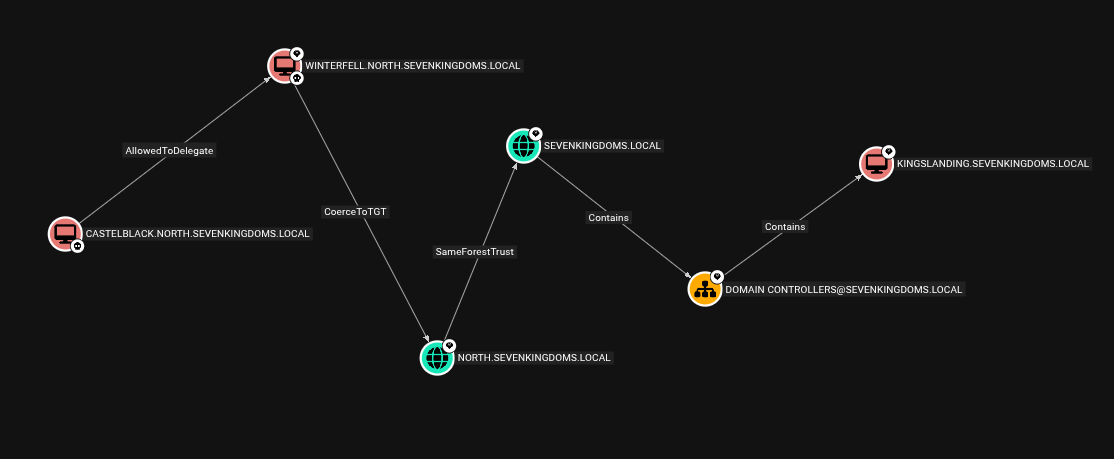
\includegraphics[width=0.9\textwidth]{ressources/bloodhound_shortest_path.png}
    \caption{BloodHound missing the memberOf edge and not finding the actual shortest path.}
    \label{fig:bh_ghost_miss}
\end{figure}
% ------------------------------------

To deterministically resolve this discrepancy, a manual audit of the 
pipeline's underlying data structures was conducted. By mapping the objects 
to their (\glspl{sid})---specifically, the 
source computer (\gls{sid}: \texttt{S-1-5-21-2466621736-3584596050-225777411-1001}) 
and the target group (\gls{sid}: \texttt{SEVENKINGDOMS.LOCAL-S-1-5-9})---a 
programmatic search of the compiled (\gls{pyg}) 
\texttt{HeteroData} tensor was executed. The audit definitively returned a 
positive match within the \texttt{('computers', 'memberof', 'groups')} edge 
index, proving the transition mathematically exists within the collected 
ground truth.

The absence of this edge within the BloodHound \gls{gui} highlights a critical 
vulnerability in relying exclusively on presentation-layer tools. While the 
backend Neo4j database likely ingested the relationship from the raw 
\texttt{bloodhound-python} scans, the BloodHound frontend employs restrictive 
Cypher query heuristics and visual filtering. To prevent browser memory 
exhaustion and UI clutter (the ``hairball'' effect), the application 
frequently truncates cross-domain nested group memberships or excludes 
universal well-known \glspl{sid} from its default shortest-path calculations. 

This anomaly demonstrates a significant operational advantage of deploying deep 
learning directly against the raw tensor structure. The 
\texttt{GNN-AD-Navigator} operates exclusively on the unrolled mathematical 
matrices, it is entirely immune to the visual filtering constraints and 
hardcoded query limitations of frontend applications. It successfully 
surfaces stealthy, structurally valid ``ghost edges'' that a human operator 
relying solely on standard visualisation interfaces would completely overlook.

\section{Result 3: Constrained Delegation}
\label{sec:result3}

\begin{lstlisting}[language={}, caption={Model output on unseen node}, label={lst:trust_output}]
Start  : castelblack.north.sevenkingdoms.local (computers)
Target : kingslanding.sevenkingdoms.local (computers)

Path 1:
  Score: 1.0000  Steps: 2
    [1] castelblack.north.sevenkingdoms.local
        -> winterfell.north.sevenkingdoms.local
        edge   : allowedtodelegate
        attack : Constrained Delegation
        action : S4U2Self + S4U2Proxy impersonation
    [2] winterfell.north.sevenkingdoms.local
        -> enterprise domain controllers@sevenkingdoms.local
        edge   : memberof
        attack : Group inheritance
        action : Inherit rights via group membership

  AUDIT:
     Path terminates at a node with DCSync on the target domain 'kingslanding.sevenkingdoms.local'. This is operational success.
\end{lstlisting}

A key insight to foreground is that the \texttt{AllowedToDelegate} edge was 
missed during the graph construction during training. The 
\texttt{AllowedToDelegate} is an edge type not directly present in the raw 
BloodHound scan; it needed further processing, deducing the relationship 
between the two nodes before establishing its existence. Hence, during 
training, the model did not see this edge type. When introduced for this 
query as the only navigable node, the model successfully suggested traversing 
it and gave a score of 1.0 (the only probable path). 

Notably, this phenomenon was not isolated to constrained delegation; the exact 
same behaviour was observed with the \texttt{CoerceToTGT} edge, which was 
also successfully traversed despite being invisible during the training phase. 
Furthermore, this dynamic highlights a structural advantage of the pipeline: 
by manually modifying the heuristic weights of these once-invisible edges 
during inference, an operator can directly affect the model's navigation. 
Tuning these weights forces the beam search to either prioritise or penalise 
these specific, newly-discovered attack techniques based on the red team's 
operational context.

% ─────────────────────────────────────────────────────────────
\section{Result 4: Documented Limitations}
\label{sec:result4}

While the zero-shot evaluation on INLANEFREIGHT demonstrated significant 
operational capability, the diagnostic queries also exposed structural 
limitations within the pipeline. These limitations stem primarily from the 
nature of heuristic beam search algorithms and the distribution of the 
supervised training data.

\subsection{Heuristic Divergence and Terminal State Blindness}

A query from \texttt{castelblack.north.sevenkingdoms.local} to 
\texttt{braavos.essos.local} produced an interesting topological divergence 
between the model's output and BloodHound's native pathfinding. 

The \texttt{GNN-AD-Navigator} navigated the following route: 
\texttt{castelblack} $\rightarrow$ \texttt{winterfell} 
(\texttt{AllowedToDelegate}) $\rightarrow$ \texttt{enterprise domain 
controllers@sevenkingdoms} (\texttt{MemberOf}) $\rightarrow$ 
\texttt{sevenkingdoms.local} (\texttt{GetChanges}, partial DCSync) 
$\rightarrow$ \texttt{essos.local} (\texttt{CrossForestTrust}) 
$\rightarrow$ \texttt{laps@essos} (\texttt{Contains}) $\rightarrow$ 
\texttt{braavos.essos.local} (\texttt{Contains}).

Conversely, BloodHound identified a structurally different route passing 
through \texttt{CoerceToTGT} on \texttt{north.sevenkingdoms.local}, followed 
by a \texttt{SameForestTrust} pivot and an \gls{acl} chain through 
\texttt{tyron.lannister} (\texttt{GenericWrite}) and 
\texttt{ReadLAPSPassword} toward the target.

This divergence is explained by two factors. First, while the neural network 
demonstrated the ability to traverse \texttt{CoerceToTGT} edges in isolation 
(as seen in Section~\ref{sec:result3}), its policy head naturally biased 
toward the mathematically dominant \texttt{CrossForestTrust} vector because 
it strongly resembles the primary domain-hopping techniques seen during 
training. Second, the two \texttt{Contains} hops at the end of the model's 
path represent structural noise. The model successfully reached 
\texttt{essos.local} and acquired \gls{dcsync} rights, but it continued 
walking down the container hierarchy rather than halting and recommending 
impersonation. This behaviour explicitly reflects the ``terminal state 
blindness'' discussed earlier, where the model struggles to recognise when 
sufficient privileges have been acquired to conclude the attack.

Neither path is strictly superior. The model relies on topological trust 
traversal, while BloodHound relies on protocol-level coercion.

\subsection{Depth Constraints and Sub-Querying}

A fundamental limitation of deploying a beam search algorithm on a graph 
exceeding 4\,000 nodes is the constraint of maximum exploration depth. During 
testing, a highly complex, stealthy attack route requiring over 10 distinct 
transitions resulted in a pipeline failure; the model returned no valid paths. 
This occurs because the beam search aggressively prunes low-probability 
branches early in the execution to save memory. If the initial steps of a 
long attack chain appear mathematically disadvantageous, the model discards 
the route before reaching the objective.

To prove that the neural architecture possessed the requisite topological 
knowledge, the objective was manually chunked into three sequential 
sub-queries, effectively providing the model with operational waypoints. As 
demonstrated in Figure~\ref{fig:subqueries}, the model successfully routed 
each of the three smaller segments with maximum confidence. This confirms 
that while the deep mathematical relationships are successfully embedded 
within the \gls{hgt} tensors, single-shot execution over exceptionally long 
horizons remains a limitation of the current beam configuration.

\begin{figure}[H]
    \centering
    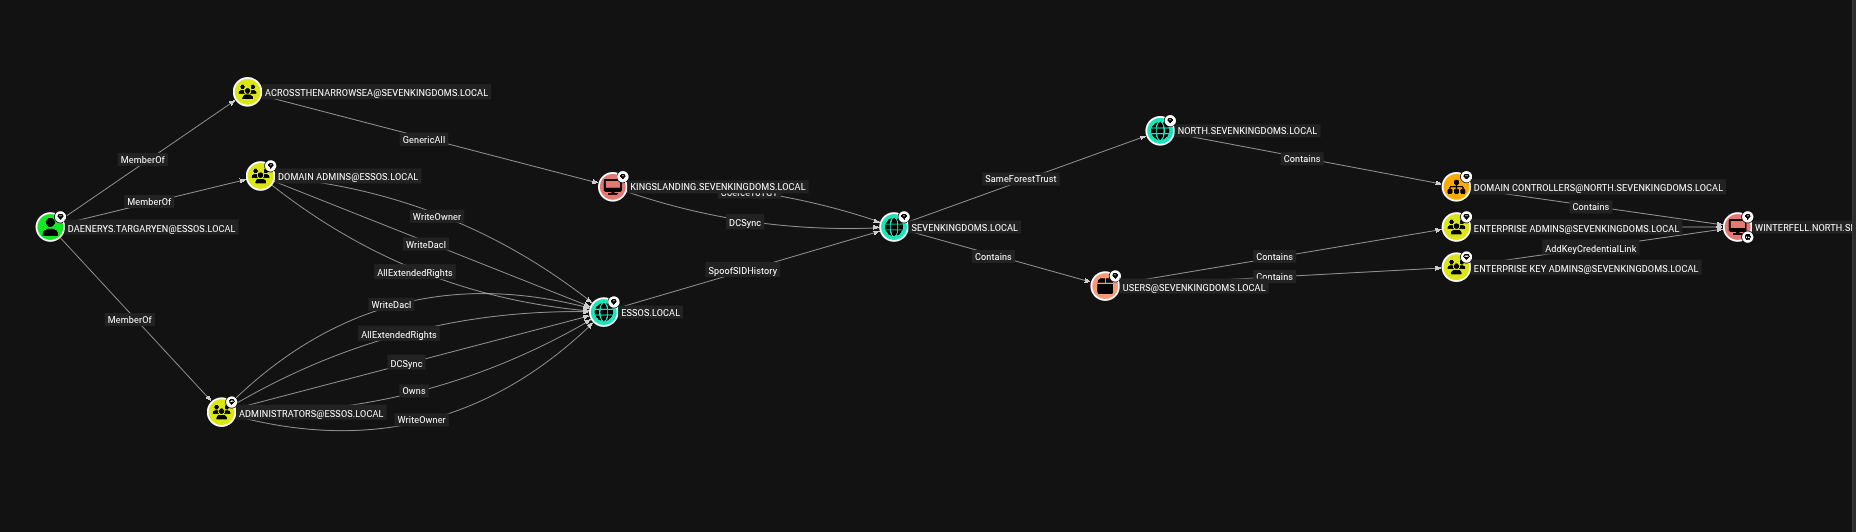
\includegraphics[width=0.9\textwidth]{ressources/long_path.png}
    \caption{The shortest path between the two nodes is 6 hopes}
    \label{fig:subqueries}
\end{figure}

\begin{lstlisting}[language={}, caption={Pipeline execution failure due to 
  structural noise and terminal state blindness}, label={lst:long_path_fail}]
Start  : daenerys.targaryen@essos.local (users)
Target : winterfell.north.sevenkingdoms.local (computers)

============================================================
RESULTS — top 3 path(s)
============================================================

Path 1:
  Score: 0.0478  Steps: 6
    [1] daenerys.targaryen@essos.local
        → domain admins@essos.local
        edge   : memberof
        attack : Group inheritance (Inherit rights via group membership)
    [2] domain admins@essos.local
        → default domain controllers policy@essos.local
        edge   : owns
        attack : Object ownership (Modify DACL of owned object)
    [3] default domain controllers policy@essos.local
        → domain controllers@essos.local
        edge   : gplink
        attack : Unknown edge (Manual review)
    [4] domain controllers@essos.local
        → meereen.essos.local
        edge   : contains
        attack : Container hierarchy (Object lives inside OU/container)
    [5] meereen.essos.local
        → enterprise domain controllers@essos.local
        edge   : memberof
        attack : Group inheritance (Inherit rights via group membership)
    [6] enterprise domain controllers@essos.local
        → windows authorization access group@essos.local
        edge   : memberof
        attack : Group inheritance (Inherit rights via group membership)

  AUDIT:
    ✗ Path terminates at 'windows authorization access group@essos.local' lacking DCSync and is not the target.
\end{lstlisting}

As discussed, attempting to navigate the complete topological distance from 
the initial foothold to the final objective in a single inference execution 
frequently triggers heuristic pruning failures. Listing~\ref{lst:long_path_fail} 
demonstrates this behaviour. The beam search algorithm discards the optimal, 
stealthy route early in the execution, instead favouring highly-rewarded 
intra-domain edges that ultimately trap the model within structural container 
noise and result in an operational audit failure.

\begin{lstlisting}[language={}, caption={The tool provides the first half of the 
  path correctly}, label={lst:long_path_fail}]
Start  : daenerys.targaryen@essos.local (users)
Target : north.sevenkingdoms.local (domains)

============================================================
RESULTS — top 1 path(s)
============================================================

Path 1:
  Score: 0.0014  Steps: 5
    [1] daenerys.targaryen@essos.local
        → domain admins@essos.local
        edge   : memberof
        attack : Group inheritance (Inherit rights via group membership)
    [2] domain admins@essos.local
        → default domain policy@essos.local
        edge   : owns
        attack : Object ownership (Modify DACL of owned object)
    [3] default domain policy@essos.local
        → essos.local
        edge   : gplink
        attack : Unknown edge (Manual review)
    [4] essos.local
        → sevenkingdoms.local
        edge   : crossforesttrust
        attack : Cross-forest trust traversal (Inter-forest pivot)
    [5] sevenkingdoms.local
        → north.sevenkingdoms.local
        edge   : sameforesttrust
        attack : Same-forest trust traversal (Cross domain via SID History)

  AUDIT:
    ✓ Path reaches the requested target directly.

\end{lstlisting}

To definitively prove that the underlying \gls{hgt} embeddings possess the 
requisite topological knowledge to solve this route, the objective was 
manually segmented to bypass the beam depth constraints. Listing~\ref{lst:subquery_1} 
illustrates the first of these segmented waypoints. By breaking the path, 
the model successfully navigates the complex multi-forest trust boundary, 
bridging the Essos domain to the North domain over a precise five-step horizon.

\begin{lstlisting}[language={}, caption={The model correctly complets the path},
  label={lst:long_path_fail}]
Start  : north.sevenkingdoms.local (domains)
Target : winterfell.north.sevenkingdoms.local (computers)

============================================================
RESULTS — top 1 path(s)
============================================================

Path 1:
  Score: 0.1430  Steps: 2
    [1] north.sevenkingdoms.local
        → domain controllers@north.sevenkingdoms.local
        edge   : contains
        attack : Container hierarchy (Object lives inside OU/container)
    [2] domain controllers@north.sevenkingdoms.local
        → winterfell.north.sevenkingdoms.local
        edge   : contains
        attack : Container hierarchy (Object lives inside OU/container)

  AUDIT:
    ✓ Path reaches the requested target directly.

\end{lstlisting}

Having successfully resolved the macro-architecture of the cross-forest trust, 
a final, highly-constrained sub-query was issued to close the remaining 
topological distance to the objective. As demonstrated in 
Listing~\ref{lst:subquery_2}, providing the model with this localized waypoint 
allows it to effortlessly traverse the final container hierarchy, landing 
directly on the target computer object with maximum precision.

% ------------------------------------

\subsection{ADCS Feature Scarcity}

Finally, while the data pipeline successfully stitches \gls{adcs} attributes 
(via Certipy) into the \gls{pyg} tensors, the model struggles to prioritise 
stealthy, deep certificate escalation chains (such as ESC1 or ESC8). This is 
a direct consequence of the supervised training data distribution. 

Within the \gls{goad} training corpus, traditional \gls{acl} abuses 
(\texttt{GenericAll}, \texttt{WriteDacl}) and group inheritances are vastly 
overrepresented compared to certificate template exploitation. Because neural 
networks inherently optimise for the most frequently rewarded patterns, the 
policy head is mathematically biased against \gls{adcs} transitions. Unless 
the certificate edge is the absolute only viable path forward, the beam search 
will almost always favour a traditional \gls{rpc} or \gls{ldap} privilege 
escalation vector. Addressing this imbalance would require generating a highly 
specialised, \gls{adcs}-heavy training dataset in future iterations.


\subsection{Heuristic Pruning of Cross-Boundary Edges}
\label{sec:heuristic_pruning}

While sub-querying proved effective for bypassing depth constraints, diagnostic 
testing revealed a secondary vulnerability within the inference engine: the 
aggressive heuristic pruning of Out-of-Distribution (OOD) topological features. 
This was explicitly observed during a cross-forest evaluation originating from 
\texttt{daenerys.targaryen@essos.local} and targeting 
\texttt{kingslanding.sevenkingdoms.local}.

Topologically, a highly efficient, two-step attack path exists between these 
nodes. The user possesses a cross-forest foreign group membership to \\
\texttt{acrossthenarrowsea@sevenkingdoms.local}, which in turn holds 
\texttt{GenericAll} privileges over the target computer. However, as 
demonstrated in Listing~\ref{lst:pruning_fail}, when executed as a single 
end-to-end query, the model completely bypassed this optimal route, instead 
favouring a convoluted six-step path that ultimately failed due to terminal 
state blindness.

\begin{lstlisting}[language={}, caption={The model bypassing the optimal two-step route due to early beam pruning.}, label={lst:pruning_fail}]
Start  : daenerys.targaryen@essos.local (users)
Target : kingslanding.sevenkingdoms.local (computers)

Path 1:
  Score: 0.0478  Steps: 6
    [1] daenerys.targaryen@essos.local
        → domain admins@essos.local
        edge   : memberof
    [2] domain admins@essos.local
        → default domain controllers policy@essos.local
        edge   : owns
    [3] default domain controllers policy@essos.local
        → domain controllers@essos.local
        edge   : gplink
    [4] domain controllers@essos.local
        → meereen.essos.local
        edge   : contains
    [5] meereen.essos.local
        → enterprise domain controllers@essos.local
        edge   : memberof
    [6] enterprise domain controllers@essos.local
        → windows authorization access group@essos.local
        edge   : memberof

  AUDIT:
    ✗ Path terminates at 'windows authorization access group@essos.local' lacking DCSync and is not the target.
\end{lstlisting}

To diagnose this failure, the route was manually broken down into two isolated 
sub-queries. The output revealed that the neural policy head assigned a 
mathematical confidence score of exactly \texttt{0.0000} to the initial 
cross-forest \texttt{MemberOf} transition. Because foreign group memberships 
were statistically rare within the \gls{goad} supervised training dataset, 
the network heavily penalised the structural anomaly of a user in Domain A 
linking directly to a group in Domain B. 

This exposes a fundamental limitation of the Beam Search algorithm in 
offensive security applications. Because the search is inherently greedy, 
it evaluates cumulative probabilities at each depth step. The \texttt{0.0000} 
confidence score on the very first transition caused the algorithm to instantly 
prune the branch in favour of standard, intra-domain edges (such as the jump 
to \texttt{domain admins@essos.local}), permanently blinding the model to the 
guaranteed compromise (\texttt{Score: 1.0000}) waiting just one hop further 
down the cross-forest chain.

The mathematical origin of this \texttt{0.0000} confidence score lies in the 
interaction between the supervised training distribution and the \gls{hgt} 
embedding space. The \gls{hgt} encoder constructs node embeddings by 
aggregating local neighbourhood features. Consequently, nodes residing in 
disparate domains are projected into distinct, distant clusters within the 
high-dimensional latent space. 

To formalise this, let $h_u$ represent the latent embedding of the source 
node (e.g., the Essos-based user) and $h_v$ represent the embedding of a 
candidate next-hop node. As defined in the architecture, the policy head 
calculates a raw transition logit $z_v$ by passing the element-wise 
(Hadamard) product of these embeddings through a Multi-Layer Perceptron 
(\gls{mlp}):

\begin{equation}
    z_v = \text{MLP}(h_u \odot h_v)
\end{equation}

Because the curated training corpus heavily emphasised intra-domain group 
inheritance, the network never received positive gradient reinforcement for 
cross-forest relationships. Thus, the interaction between the distant 
embeddings of the Essos user and the SevenKingdoms group yields a 
comparatively low raw logit ($z_{cross}$).

During the final traversal evaluation, the raw logits of all valid neighbour 
transitions $\mathcal{N}(u)$ are passed through a Softmax activation function 
to generate a normalised traversal probability distribution $P(v | u)$:

\begin{equation}
    P(v | u) = \frac{\exp(z_v)}{\sum_{k \in \mathcal{N}(u)} \exp(z_k)}
\end{equation}

This equation acts as a rigorous competitive filter. When the model evaluates 
the highly familiar, explicitly rewarded intra-domain edge (the jump to 
\texttt{domain admins@essos.local}), it produces a significantly larger logit 
($z_{intra}$). Because the Softmax function exponentiates these logits, the 
large value of $\exp(z_{intra})$ completely dominates the denominator. This 
mathematical mechanism exponentially suppresses the lower cross-forest logit, 
effectively squashing its traversal probability to exactly \texttt{0.0000} 
and causing the Beam Search algorithm to instantly prune the optimal route.

% ─────────────────────────────────────────────────────────────

\section{Discussion}

\subsection{Stateful Navigation and the Coverage Ceiling}

The curation of the \gls{goad} training dataset established a strict 
operational boundary for the model. From the raw execution logs, 
approximately 49 distinct transitions were documented, which were subsequently 
filtered down to 33 purely topological, learnable attack vectors. This finite 
vocabulary directly influenced the fundamental architecture of the system.

Initial iterations of this research explored a ``stateful'' or context-aware 
policy head. This approach would have required the model to maintain an active 
inventory of compromised credentials and privileges dynamically during the 
beam search, allowing its navigation to be conditioned on acquired assets 
rather than purely spatial topology. However, implementing a recurrent or 
reinforcement-based state tracker required a massively expanded, dynamic 
training dataset that far exceeded the 33 static traces available. 

Consequently, the architecture was constrained to stateless topological 
inference. The model successfully learns the structural semantics of 
techniques like \gls{acl} abuse and \gls{dcsync}, but it cannot logically 
chain attacks that require holding a specific credential from Step A to 
execute Step D. The development of dynamic attack inventory generation is a 
natural evolution of this architecture but requires a distinct reinforcement 
learning objective and is explicitly designated as future work.

\subsection{Pipeline Dominance: Decoupling Data from Weights}

Perhaps the most significant architectural observation from the inference 
testing is the model's handling of completely unseen edge types. During 
training, the neural network never encountered \texttt{AllowedToDelegate} 
or \texttt{CoerceToTGT} primitives. Yet, once the Python data pipeline 
(\texttt{stitcher.py} and \texttt{build\_dataset.py}) was updated to extract 
and synthetically generate these relationships, the frozen model successfully 
traversed them during zero-shot inference without requiring any mathematical 
retraining.

This behaviour proves that the model's ability to discover novel attack paths 
is heavily dictated by the completeness of the data ingestion pipeline. Because 
the neural network relies on the graph's physical topology to evaluate 
contiguous sub-graphs, introducing a newly discovered \gls{ad} vulnerability 
simply translates to injecting a new structural pathway into the \gls{pyg} 
tensor. Even without learned attention weights explicitly tuned for 
\texttt{CoerceToTGT}, the policy head opted to traverse it because it 
represented a mathematically viable bridge toward the target embedding.

This decoupling of graph coverage from neural capability is a massive 
operational advantage. It implies that security teams do not need to 
recompile or retrain the deep learning architecture from scratch every time 
a novel \gls{ad} misconfiguration is published to the red-team community. 
Instead, updating the upstream json parsers to map the new technique 
into the static graph is sufficient to immediately expand the AI's 
operational reach. For this reason, the deterministic data engineering 
pipeline developed in this research is considered a primary contribution, 
functioning as a critical enabler for the underlying neural network.

%% ============================================================
%%  CHAPTER 5 — LIMITATIONS AND FUTURE WORK
%% ============================================================
\chapter{Limitations and Future Work}

While the empirical evaluation in Chapter 4 demonstrates that the 
Heterogeneous Graph Transformer \gls{hgt} successfully learns and generalises 
offensive navigation policies, the current pipeline remains a proof of 
concept. Transitioning from a controlled laboratory environment to a 
production-ready red teaming tool requires an honest assessment of the 
system's boundaries. This chapter systematically details the fundamental 
mathematical, algorithmic, and operational limitations of the current 
approach, and proposes a concrete engineering roadmap for a 
second-generation architecture.

\section{Mathematical and Algorithmic Limitations}

The most significant constraints on the GNN-AD-Navigator do not stem 
from data ingestion or environmental scanning, but from the inherent 
mechanics of deep learning when applied to complex, asymmetrical graph 
structures. Understanding these mathematical flaws is critical for 
interpreting the model's behaviour during deep attack simulations.

\subsection{Multiplicative Probability Decay and Search Bias}

The inference phase relies on a heuristic beam search to navigate the 
Active Directory graph. At each step, the policy head outputs a Softmax 
probability distribution over all available candidate edges. The total 
confidence score for a given attack path is then calculated by multiplying 
the individual probabilities of each hop along that route.

Mathematically, multiplying fractions consistently yields a smaller 
product (e.g., $0.8 \times 0.8 \times 0.8 = 0.512$). In the context of 
Active Directory attack paths, this creates a phenomenon known as 
\textit{multiplicative probability decay}. The search algorithm 
inherently penalises long attack chains simply because they require more 
mathematical transitions.

From an offensive security perspective, this mathematical decay directly 
contradicts the foundational objective of the navigation policy. The primary 
motivation for engineering transition-specific confidence scores---effectively 
acting as an \gls{OPSEC} step cost---was to explicitly train 
the model to prioritise stealth over path efficiency. In professional red 
teaming engagements, operators heavily rely on \gls{lotl}
techniques, deliberately chaining multiple low-privilege, native Active 
Directory misconfigurations to escalate privileges without triggering \gls{siem} 
(Security Information and Event Management) alarms. The model was designed to 
recognise these stealthy, deep attack chains as operationally superior to a 
noisy, direct exploit. However, because the probability decay compounds with 
every additional transition, the mathematical penalty of path length 
eventually overwhelms the learned OPSEC rewards. As a result, the beam 
search prematurely prunes the desired stealthy chains, paradoxically forcing the 
model to revert to the exact behaviour it was engineered to avoid: 
demonstrating a strong preference for shorter, highly detectable attacks 
simply because they require fewer algorithmic multiplications.

\subsection{Bounded Receptive Field and the Horizon Problem}

The expressiveness of a Graph Neural Network is fundamentally tied to its 
receptive field, which is dictated by the number of hidden layers ($K$). 
During the message-passing phase, a node aggregates feature data from $K$ 
hops away. Therefore, to intrinsically understand the structural relationship 
between a compromised starting user and a target Domain Controller seven 
steps away, the model would theoretically require seven layers of message 
passing.

However, Active Directory environments are highly dense, "small world" 
networks, characterised by heavily nested group memberships and extensive 
permissions. In such dense topologies, expanding the depth of the 
network triggers a well-documented graph learning limitation known as 
\textit{over-smoothing}. If the Heterogeneous Graph Transformer \gls{hgt} is 
configured with too many layers, the repeated aggregation of neighbourhood 
features causes the embeddings of structurally distinct nodes---such as a 
standard workstation and an Enterprise Admin group---to mathematically 
converge toward indistinguishable mean vectors.

To preserve the distinct privilege hierarchies required for accurate 
routing, the GNN-AD-Navigator's architecture is strictly bounded to a 
shallow depth (specifically $K=2$ layers, as established in the methodology). 
While this successfully prevents over-smoothing and maintains structural 
fidelity, it directly introduces the \textit{horizon problem}. When 
executing a deep attack simulation (e.g., a 7-hop path), the starting 
node's embedding contains zero latent information about a target that lies 
beyond its two-hop receptive field. The policy head is effectively blind 
to the distant destination, forcing the algorithm to navigate using only 
local privilege gradients rather than true, end-to-end topological 
awareness.

\subsection{The "Blind Compass" Effect in Lateral Movement}

As detailed in Chapter 2, a critical engineering adaptation within the 
pipeline was the design of the policy head. Rather than computing a 
target-aware concatenation, the model utilises the Hadamard product 
(element-wise multiplication) between the current node's embedding and the 
candidate neighbour's embedding. This architectural choice proved highly 
effective for the primary goal of Active Directory exploitation: privilege 
escalation. By forcing the model to evaluate the absolute semantic value of a 
transition, it successfully learned a generalised privilege hierarchy. It acts 
as a "universal climber" that inherently gravitates toward high-value nodes 
like Domain Admins, regardless of the specific topology.

However, this adaptation introduces a distinct operational trade-off. Because 
the target node's embedding is mathematically excluded from the transition 
scoring, the policy head possesses no "target gravity." The model implicitly 
knows how to escalate privileges, but it does not inherently know its final 
destination. 

This limitation becomes acutely apparent during horizontal lateral movement. 
If an attack simulation requires navigating through a flat network segment---
such as pivoting between multiple standard workstations within an isolated 
Organizational Unit (OU)---the model struggles to find an optimal route. When 
presented with candidate neighbours that share identical, low-privilege 
weights, the policy head lacks the directional context required to efficiently 
break the mathematical tie. Without the target vector actively pulling the 
algorithm toward a specific coordinate, the search can oscillate or wander 
inefficiently. The model effectively acts as a "blind compass"---perfectly 
calibrated to point "up" toward domain dominance, but unable to navigate 
laterally toward a specific, non-administrative target.

\section{Operational and Data Boundaries}

A fundamental axiom of machine learning is that a model's operational 
capacity is strictly bounded by the fidelity of its underlying data. While 
the algorithmic limitations define how the model navigates the graph, the 
operational boundaries dictate whether the necessary topological pathways 
exist in the underlying dataset to begin with.

\subsection{Edge Directionality and the Computer Node Sinkhole}

During the empirical evaluation, the model occasionally exhibited suboptimal 
routing by bypassing topologically logical hops through specific Computer 
nodes. This behaviour is not an algorithmic failure, but rather a direct 
consequence of how \texttt{PyTorch Geometric} enforces strict edge 
directionality, combined with the inherent nature of Active Directory 
Access Control Lists (ACLs).

In a standard BloodHound-compatible graph, privileges are mapped as directed 
edges from a principal (the controller) to a target (the controlled). 
Consequently, Computer nodes predominantly accumulate incoming edges (e.g., 
Users or Groups holding \texttt{GenericAll} or \texttt{AdminTo} rights over 
the machine) but possess virtually zero outgoing rights over other objects in 
the domain. Without the ability to dynamically resolve and traverse active 
user sessions (e.g., using a \texttt{HasSession} edge to pivot from the 
compromised machine to a highly privileged Domain Admin logged into it), the 
Computer node becomes a topological sinkhole. 

The inference engine mathematically learns to avoid these nodes because 
traversing into them almost always results in a dead end. While a human 
operator would compromise the computer, dump memory credentials (e.g., via 
Mimikatz), and pivot, the current graph schema does not explicitly represent 
that post-exploitation capability as a traversable outgoing edge.

\subsection{Collector Incompleteness and Schema Evolution}

The current data pipeline relies heavily on the Linux-compatible Python 
ingestor (\texttt{bloodhound-ce-python}). While this ensures the toolset 
remains accessible from standard UNIX-based attack hosts, it introduces 
severe structural blind spots. Most notably, the Python collector exhibits 
incompleteness regarding  the enumeration of explicit Trust accounts. Furthermore, 
it lacks native support for Active Directory Certificate Services (ADCS), 
necessitating reliance on legacy versions of \texttt{Certipy} and complex logic
to stitch the graph together.

This fragility was 
further exacerbated by environmental volatility during graph enumeration 
phases. For example, hypervisor kernel incompatibilities and virtual network 
bridging failures during the provisioning of the \texttt{ESSOS.local} test 
domain demonstrated that relying on fragmented, multi-tool data collection 
is difficult to scale consistently.

Ultimately, this is an ingestion constraint, not a model limitation. For a 
production-grade deployment, future iterations must deprecate the Python 
ingestor in favour of the official C\# SharpHound collector. Executing 
SharpHound natively within the target environment would inherently surface 
coercion-derived edges, complete trust mappings, and richer ACL enumeration, 
directly expanding the model's discoverable attack surface without requiring 
any architectural modifications to the neural network.

\subsection{ADCS Edge Sparsity and Static Stitching}

The current dataset exhibits severe class imbalance regarding \gls{adcs} 
attack primitives. Within the training corpus, 
\gls{adcs} template transitions---such as \texttt{Enroll} or 
\texttt{WriteDacl} over a \texttt{CertTemplate} node---are extremely 
scarce, typically limited to only one or two traversable instances per 
template. 

From a deep learning perspective, this edge sparsity presents a significant 
challenge for the \gls{hgt}. Neural networks 
require sufficient statistical frequency to accurately learn the latent 
semantic weight of a transition. Because the model observes thousands of 
\texttt{MemberOf} or \texttt{GenericAll} relationships but only a handful 
of \gls{adcs} escalations, the policy head inherently struggles to assign 
an operationally confident probability score to certificate-based attacks 
during inference, occasionally causing the beam search to undervalue them.

Furthermore, this sparsity is compounded by the pipeline's ingestion 
mechanics. Because the Python collector natively lack comprehensive 
\gls{adcs} enumeration, these specific edges are currently extracted via 
fragmented \texttt{Certipy} scans and statically stitched into the 
underlying graph using custom Python logic. While this static injection 
successfully bridges the topological gap and physically allows the model 
to traverse the \gls{adcs} infrastructure, the hardcoded nature of the 
stitching process remains brittle. Future iterations must address this 
data scarcity---either through the injection of synthetic \gls{adcs} 
traces to artificially amplify the training signal, or by adopting a 
unified, native collection tool that reliably surfaces certificate 
misconfigurations at scale.

\section{Future Work: Algorithmic Upgrades}

The mathematical constraints identified in Section 5.1 cannot be resolved 
simply by increasing the volume of training data or arbitrarily tuning 
hyperparameters. Addressing the horizon problem and the adverse effects of 
multiplicative probability decay requires fundamental architectural 
enhancements to the inference engine. The following algorithmic upgrades 
outline a clear engineering roadmap for a second-generation navigation 
tool, focusing on hybridizing deep learning embeddings with deterministic 
routing logic.

\subsection{Waypoint Routing and Path Segmentation}

To overcome the bounded receptive field of the Heterogeneous Graph 
Transformer, future iterations of the pipeline should implement a 
"divide-and-conquer" routing wrapper. As previously established, the 
model struggles with deep attack chains because targets beyond a two-hop 
radius fall completely outside the starting node's latent awareness, 
creating a blind horizon.

A waypoint routing architecture would solve this by decoupling the global 
pathfinding strategy from the local transition predictions. Much like 
modern GPS navigation systems, a static pre-processor could analyse the 
global graph topology to identify major structural hubs or "choke points"---
such as highly connected \gls{ou}, Tier-0 infrastructure, or centralized 
identity providers. 

Instead of querying the neural network to calculate a continuous, 10-hop 
path from a low-privileged user directly to a Domain Controller, the 
wrapper would segment the objective. The model would first be tasked with 
navigating to the nearest waypoint; upon success, the search state would 
reset and generate a new trajectory to the subsequent waypoint. 

This segmentation directly neutralises both the horizon problem and the 
multiplicative probability decay. By ensuring that each individual path 
segment remains short, the intermediate targets stay within the model's 
receptive field. Furthermore, resetting the probability calculation at 
each waypoint prevents the accumulated mathematical penalties from 
overwhelming the learned \gls{OPSEC} step costs, allowing the model to freely 
select stealthy, non-linear routes.

\subsection{Guided Search Heuristics ($A^*$ Algorithm)}

While waypoint routing mitigates the horizon problem, the fundamental 
inference mechanism must also evolve to protect OPSEC-driven routing. The 
current implementation relies on a heuristic beam search, which, as 
established, falls victim to multiplicative probability decay. To preserve 
long, stealthy attack chains, future architectures should replace the pure 
beam search with an additive, cost-based heuristic algorithm such as $A^*$ 
(A-Star).

Unlike beam search, which evaluates routes by multiplying fractional Softmax 
probabilities, $A^*$ evaluates candidate paths using an additive cost 
function: $f(n) = g(n) + h(n)$. In this paradigm, $g(n)$ represents the 
exact, accumulated OPSEC cost of the path taken so far, while $h(n)$ serves 
as the heuristic estimating the remaining distance or effort to the target. 
By summing step costs rather than multiplying probabilities, the mathematical 
penalty for path length grows linearly rather than exponentially. 

This algorithmic shift would elegantly repurpose the existing deep learning 
architecture. Instead of acting as a standalone, greedy pathfinder, the 
\gls{hgt} policy head would be deployed 
exclusively as the heuristic function, $h(n)$. The \gls{gnn} would evaluate 
candidate neighbours and assign dynamic, context-aware proximity scores based 
on learned privilege hierarchies, while the deterministic $A^*$ framework 
strictly tracks the accumulated stealth metrics ($g(n)$). 

This hybrid approach ensures that operationally superior, low-privilege 
\gls{lotl} chains are evaluated on their true tactical 
merit. It mathematically protects longer paths from being prematurely pruned, 
completely eradicating the current system's bias toward short, highly 
detectable exploit paths.

\subsection{Terminal State Learning and Global Reachability}

The current inference engine relies on a hardcoded symbolic predicate to 
identify terminal states: if the search algorithm lands on a node possessing 
\gls{dcsync} rights (e.g., \texttt{GetChanges} and \texttt{GetChangesAll} on the 
target domain), the search halts, assuming total domain compromise. While 
theoretically rudimentary, the empirical results from Chapter 4 demonstrate 
that this static cutoff condition is operationally sufficient and highly 
effective for current red teaming engagements.

A theoretically purer approach would involve replacing this hardcoded 
heuristic with Offline \gls{rl}. By training a dedicated 
value head over the existing traces using algorithms like Conservative 
Q-Learning (CQL), the model could intrinsically learn to assign massive 
reward values to DCSync-capable nodes. However, deploying an Offline RL 
architecture is exceptionally complex, computationally expensive, and prone 
to severe training instability. Given the high performance of the current 
static condition, introducing a brittle RL pipeline represents significant 
engineering overhead for diminishing returns.

A more pragmatic, data-driven alternative exists to teach the policy head 
the concept of global reachability without altering the underlying 
architecture. The training corpus could be augmented with synthetic traces 
where reaching a DCSync-capable node is immediately followed by a direct 
transition to the final target, regardless of whether a literal topological 
edge exists. By exposing the model to these synthetic "teleportation" 
transitions, the \gls{hgt} would mathematically 
learn that owning a \gls{dcsync} node equates to owning the entire graph. This 
allows the existing architecture to organically learn the semantic weight 
of domain dominance entirely through data representation, bypassing the need 
for a resource-heavy Reinforcement Learning overhaul.

\subsection{LLM Integration for Out-Of-Vocabulary (OOV) Edges}

As offensive enumeration tools like SharpHound evolve, their output schemas 
and edge vocabularies frequently change (e.g., introducing new attack 
primitives or altering nomenclature such as \texttt{WriteDACL} to 
\texttt{WriteDacl}). The current pipeline relies on a static alias mapping 
dictionary to normalise these relationships before tensor vectorisation. 
From an engineering perspective, this static approach is highly efficient, 
computationally lightweight, and operationally sufficient for the current 
Active Directory landscape.

However, maintaining a hardcoded vocabulary introduces long-term technical 
debt and fragility when encountering undocumented, \gls{oov} 
edges during a live engagement. A promising future direction is the 
integration of a localized, lightweight Large Language Model (LLM) to act 
as a semantic parser at the ingestion layer. Instead of dropping or ignoring 
unknown relationships, the LLM could semantically evaluate the new edge type 
and automatically map it to the closest known privilege vector in the 
model's latent space. While static mappings are entirely sufficient for 
today's red teaming operations, LLM-assisted parsing would provide a highly 
resilient, future-proof ingestion pipeline capable of organically adapting 
to evolving Active Directory schemas.


\section{Conclusion}

The limitations and proposed upgrades outlined in this chapter do not 
diminish the empirical success of the current \texttt{GNN-AD-Navigator}; 
rather, they define the precise engineering trajectory required to transition 
from a constrained proof-of-concept to an enterprise-grade autonomous 
agent. 

An application that successfully surpasses these boundaries---coupling 
the deep semantic embeddings of a Heterogeneous Graph Transformer with the 
deterministic routing of an $A^*$ heuristic and localised waypoint 
segmentation---would represent a paradigm shift in automated offensive 
security. Such a system would prove that AI-driven pathfinding can scale to 
massive, asymmetrical Active Directory environments without sacrificing the 
OPSEC requirements crucial for advanced \gls{lotl} attack 
chains. It would effectively transition automated red teaming from rigid, 
shortest-path vulnerability scanners into dynamic, stealth-conditioned 
navigators.

More broadly, this research roadmap redefines the role of Graph Neural 
Networks in the cybersecurity domain. Historically relegated to defensive 
classification tasks, such as anomaly detection or alert clustering, this 
work establishes \glspl{gnn} as foundational reasoning engines for offensive 
operations. By proving that neural networks can mathematically abstract 
and internalise the semantic hierarchy of privilege escalation, it lays 
the theoretical groundwork for a new generation of agentic AI---tools 
capable of navigating complex digital topologies with the intuitive, 
contextual awareness of a human Red Teamer.

%% ============================================================
%%  GENERAL CONCLUSION
%% ============================================================
\chapter*{General Conclusion}
\addcontentsline{toc}{chapter}{General Conclusion}
\markboth{General Conclusion}{}

This thesis presented the design, implementation, and empirical evaluation of 
the \texttt{GNN-AD-Navigator}, an end-to-end, deep learning-driven pipeline 
for automated Active Directory privilege escalation. By bridging the gap 
between offensive security data collection and advanced graph representation 
learning, the architecture successfully translated raw BloodHound json 
fragments into compiled PyTorch Geometric (\gls{pyg}) tensors. Through the 
application of a Heterogeneous Graph Transformer (\gls{hgt}) and a tailored 
heuristic beam search algorithm, the model demonstrated the capacity to 
autonomously navigate complex enterprise topologies, ultimately surfacing 
highly stealthy attack paths via a streamlined Streamlit graphical interface.

The research yielded three highly defensible operational contributions. First, 
the architecture demonstrated exceptional zero-shot generalisation. When 
deployed against the previously unseen, 4\,000-node INLANEFREIGHT enterprise 
environment, the model successfully routed unprivileged footholds to 
\gls{dcsync} capabilities across multi-domain trust boundaries. Second, the 
research exposed the ``Ghost Edge'' anomaly, proving that by operating 
directly on the unrolled mathematical tensors, the neural network could 
surface stealthy cross-domain relationships that the industry-standard 
BloodHound \gls{gui} completely failed to render due to presentation-layer 
heuristics. Finally, the evaluation highlighted the principle of pipeline 
dominance: the discovery that updating the Python ingestion pipeline to 
recognise novel edges (such as \texttt{AllowedToDelegate}) immediately 
unlocked new traversal capabilities without requiring the neural network 
weights to be retrained.

Crucially, this work maintains an honest appraisal of its operational scope. 
The system functions as a highly advanced proof-of-concept constrained by its 
training distribution. The 33 curated topological traces extracted from the 
\gls{goad} environment define a strict coverage ceiling. The model operates 
with high precision within these bounds but exhibits documented failure states 
when pushed beyond them. Limitations such as beam search depth constraints, 
the heuristic pruning of Out-of-Distribution cross-forest edges, and terminal 
state blindness clearly illustrate the boundaries of stateless topological 
inference. The architecture is not broken; rather, it behaves exactly as its 
mathematical configuration dictates at the edge of its coverage.

Ultimately, these identified limitations provide a clear, structured roadmap 
for future research. The transition from stateless topology mapping to 
stateful, context-aware navigation via Reinforcement Learning represents the 
most significant avenue for evolution. Furthermore, expanding the supervised 
training corpus to heavily weight \gls{adcs} certificate abuse, alongside 
hardening the data engineering pipeline to enforce strict cross-forest 
protocol boundaries, will directly address the current edge cases. This 
thesis does not represent a final, exhaustive product, but rather a robust, 
academically rigorous foundation for the next generation of AI-driven 
offensive security tooling.


%% ============================================================
%%  BIBLIOGRAPHY
%% ============================================================
\printbibliography[heading=bibintoc, title={Bibliography}]


%% ============================================================
%%  APPENDICES
%% ============================================================
\appendix
\chapter{Sanitised BloodHound JSON}
\label{app:json_example}

The following snippet demonstrates the structural schema of the raw BloodHound 
JSON data before it is ingested and vectorised by the data pipeline. Extraneous 
metadata (such as timestamps, unpopulated arrays, and logon statistics) has 
been omitted for brevity. 

This specific example highlights a user object (\texttt{drogon@essos.local}) 
and demonstrates how topological relationships (such as a \texttt{GenericAll} 
edge) are stored within the \texttt{Aces} array prior to being mapped into 
the \texttt{HeteroData} edge indices.

\begin{lstlisting}[language={}, caption={Truncated and sanitised JSON structure for a User node.}, label={lst:json_snippet}]
{
  "users": [
    {
      "ObjectIdentifier": "S-1-5-21-3939323223-2065505069-2611713634-1118",
      "Properties": {
        "name": "drogon@essos.local",
        "domain": "essos.local",
        "highvalue": false,
        "sensitive": false,
        "admincount": true,
        "unconstraineddelegation": false
      },
      "Aces": [
        {
          "PrincipalSID": "S-1-5-21-3939323223-2065505069-2611713634-512",
          "PrincipalType": "Group",
          "RightName": "GenericAll",
          "IsInherited": false
        }
      ],
      "HasMember": [],
      "MemberOf": []
    }
  ]
}
\end{lstlisting}

\chapter{Heterogeneous Graph Schema}
\label{app:schema}

This appendix details the structural schema of the PyTorch Geometric (\gls{pyg}) 
\texttt{HeteroData} object utilised by the \texttt{GNN-AD-Navigator}. The graph 
is inherently heterogeneous, comprising multiple distinct node and edge types 
derived from the merged Active Directory environment.

\section{Node Schema}
The compiled graph consists of 7 distinct node types. To ensure dimensional 
consistency across the Heterogeneous Graph Transformer (\gls{hgt}) layers 
during message passing, every node type is embedded with a uniform feature 
vector of size 14.

\begin{table}[H]
    \centering
    \begin{tabular}{lcc}
        \toprule
        \textbf{Node Type} & \textbf{Node Count (GOAD)} & \textbf{Feature Dimension} \\
        \midrule
        \texttt{users} & 48 & 14 \\
        \texttt{groups} & 166 & 14 \\
        \texttt{computers} & 5 & 14 \\
        \texttt{domains} & 3 & 14 \\
        \texttt{ous} & 12 & 14 \\
        \texttt{gpos} & 8 & 14 \\
        \texttt{containers} & 66 & 14 \\
        \bottomrule
    \end{tabular}
    \caption{Node types, dataset distributions, and their corresponding feature 
    dimensions within the PyG tensor.}
    \label{tab:node_schema}
\end{table}

\section{Edge Schema}
The \gls{hgt} architecture processes directed relationships as distinct triplets 
in the format \texttt{(source\_type, edge\_type, target\_type)}. Due to the 
mathematical permutation of Active Directory privileges across different objects 
(e.g., a \texttt{GenericAll} edge can originate from a user, a group, or a 
computer), the complete training dataset contains 75 unique edge triplets. 

Table~\ref{tab:edge_schema} provides a representative sample of these critical 
transitions extracted directly from the \texttt{HeteroData} edge indices.

\begin{table}[H]
    \centering
    \begin{tabular}{lll}
        \toprule
        \textbf{Source Node} & \textbf{Edge / Attack Type} & \textbf{Target Node} \\
        \midrule
        \texttt{users} & \texttt{allowedtodelegate} & \texttt{computers} \\
        \texttt{groups} & \texttt{genericall} & \texttt{users} \\
        \texttt{groups} & \texttt{addkeycredentiallink} & \texttt{users} \\
        \texttt{users} & \texttt{genericwrite} & \texttt{users} \\
        \texttt{users} & \texttt{forcechangepassword} & \texttt{users} \\
        \texttt{groups} & \texttt{readgmsapassword} & \texttt{users} \\
        \texttt{computers} & \texttt{readgmsapassword} & \texttt{users} \\
        \texttt{groups} & \texttt{owns} & \texttt{computers} \\
        \texttt{groups} & \texttt{writedacl} & \texttt{users} \\
        \bottomrule
    \end{tabular}
    \caption{A representative subset of the 75 directional edge triplets processed 
    by the neural policy head.}
    \label{tab:edge_schema}
\end{table}

\chapter{Key Code Excerpts}
\label{app:code}

\section*{Effective Weight Loss Function}
\begin{lstlisting}[language=Python, caption={Effective weight computation in \tool{prepare\_training\_examples.py}}]
# eff_weight combines path importance with step discretion cost
eff_weight = path_weight * (1 - step_cost)
\end{lstlisting}
\section*{DCSync Validation Logic}
The \texttt{has\_dcsync\_on} function mathematically verifies if a node has acquired the requisite combination of rights (\texttt{GetChanges} and either \texttt{GetChangesAll} or \texttt{GetChangesInFilteredSet}) to perform a DCSync attack against the target domain.

\begin{lstlisting}[language=Python, caption={Terminal state validation for DCSync execution in \tool{inference.py}}, label={lst:dcsync_check}]
def has_dcsync_on(node_idx, target_domain_name, edge_tensors_flat, idx_to_name):
    held_on = set()
    for rel in DCSYNC_RIGHTS:
        ei = edge_tensors_flat.get(rel)
        if ei is None: continue
        src, dst = ei
        mask = (src == node_idx)
        for d in dst[mask].tolist(): held_on.add((rel, idx_to_name.get(d, "")))

    has_getchanges    = {d for r, d in held_on if r == "getchanges"}
    has_getchangesall = {d for r, d in held_on if r == "getchangesall"}
    has_filtered      = {d for r, d in held_on if r == "getchangesinfilteredset"}

    domains_with_both = has_getchanges & (has_getchangesall | has_filtered)
    won = False
    for d in domains_with_both:
        if target_domain_name == d or target_domain_name.endswith("." + d):
            won = True; break
    return won, list(domains_with_both)
\end{lstlisting}

\section*{Heuristic Beam Search Core Loop}
This excerpt highlights the core navigation loop of the inference engine. It demonstrates the neural policy head scoring candidate neighbours, applying the Softmax activation, and the critical fallback bypass mechanism used to prevent the pruning of Out-of-Distribution (OOD) edges.

\begin{lstlisting}[language=Python, caption={The iterative beam search and scoring loop in \tool{inference.py}}, label={lst:beam_search}]
def beam_search(model, embeddings, edge_tensors_flat, start_idx, target_idx, idx_to_name, edge_name_map, known_edges, beam_width=3, max_depth=8):
    target_domain = get_node_domain(target_idx, idx_to_name) or ""
    beam = [(0.0, [start_idx])]
    completed = []
    
    for _ in range(max_depth):
        candidates = []
        for log_score, path in beam:
            cur = path[-1]
            won, _ = has_dcsync_on(cur, target_domain, edge_tensors_flat, idx_to_name)
            
            if cur == target_idx or won:
                completed.append((log_score, path))
                continue
                
            nbrs = get_neighbors(cur, edge_tensors_flat)
            nbrs = [n for n in nbrs if n not in path and n < embeddings.shape[0]]
            if not nbrs: continue
            
            with torch.no_grad():
                scores = model.score(embeddings, cur, nbrs)
                probs  = F.softmax(scores, dim=0)
                
            for i, nb in enumerate(nbrs):
                # 1. Identify the relationship type
                rel = edge_name_map.get((cur, nb), "unknown")
                
                # 2. THE FALLBACK BYPASS
                # If the model has never seen this edge during training, bypass the 
                # neural network's score and assign it a low baseline operational score.
                if rel not in known_edges:
                    prob_val = 0.05
                else:
                    prob_val = probs[i].item()
                    
                # 3. Calculate the new sequence score
                ns = log_score + math.log(prob_val + 1e-9)
                new_path = path + [nb]
                candidates.append((ns, new_path))
                    
        if not candidates: break
        candidates.sort(key=lambda x: x[0], reverse=True)
        beam = candidates[:beam_width]
        if len(completed) >= beam_width: break
        
    # (Results sorting and trimming omitted for brevity)
    return trimmed
\end{lstlisting}

\chapter{Interface and Visualisation}
\label{app:gui}

This appendix showcases the operational interfaces developed for the 
\texttt{GNN-AD-Navigator}. To ensure the underlying PyTorch Geometric models 
are accessible for practical security assessments, both a streamlined 
Command-Line Interface (\gls{cli}) and an interactive graphical web dashboard 
were engineered.

\section{Command-Line Interface}
The \gls{cli} is designed for headless server environments and automated 
scripting. It handles the entire pipeline—from data ingestion and tensor 
compilation to heuristic beam search inference—while logging deterministic 
audit results securely to the disk.

\begin{figure}[H]
    \centering
    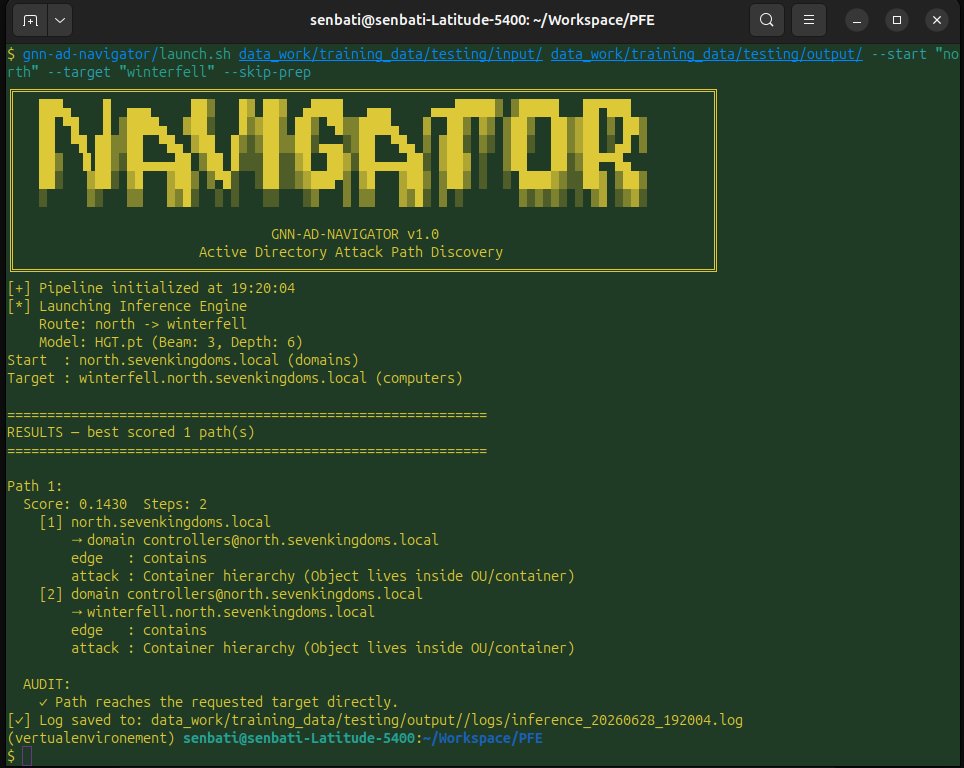
\includegraphics[width=0.9\textwidth]{ressources/cli.png}
    \caption{The streamlined \gls{cli} executing a query}
    \label{fig:cli_interface}
\end{figure}

\section{Streamlit Graphical Interface}
For human-driven analysis, a Streamlit-based web interface provides dynamic 
visualisation of the \gls{hgt} outputs. The dashboard allows operators to 
tune beam search parameters on the fly and interactively explore the generated 
attack paths via embedded \texttt{pyvis} network graphs.

\begin{figure}[H]
    \centering
    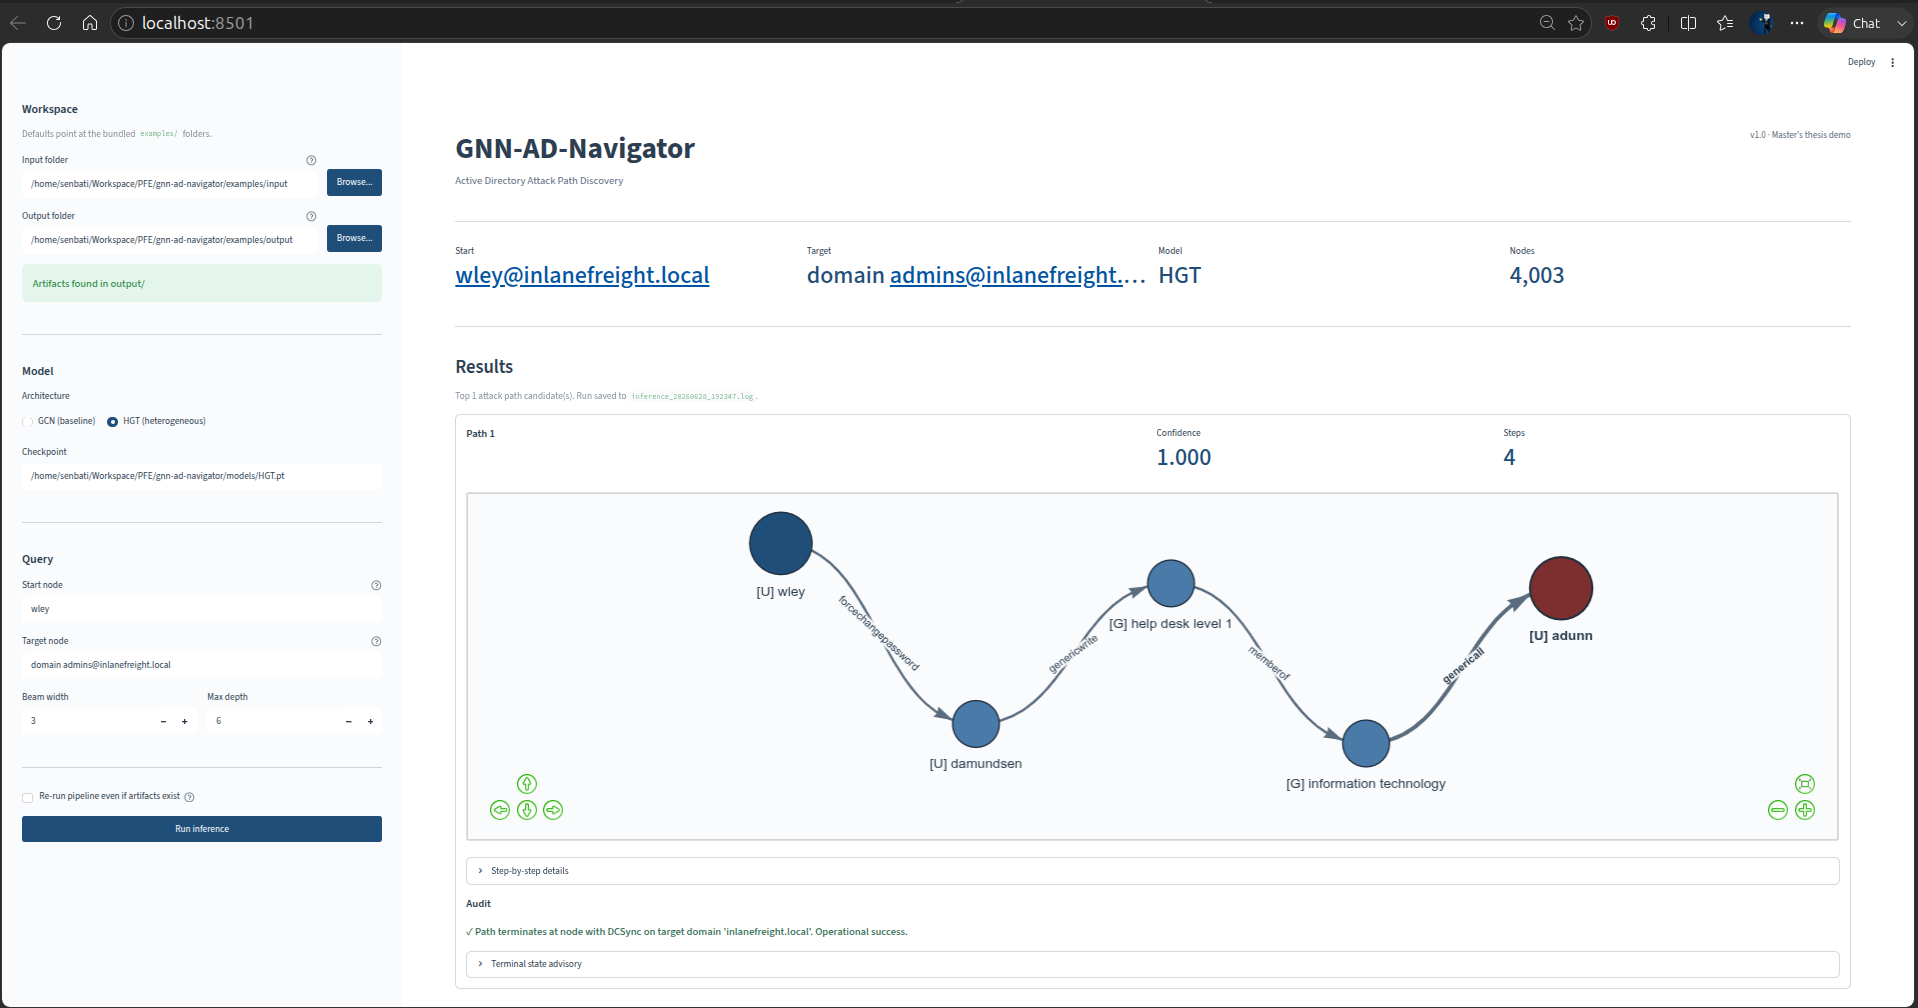
\includegraphics[width=\textwidth]{ressources/gui.png}
    \caption{The main dashboard rendering path from 
    \texttt{wley} to Domain Admin in the 4\,000-node INLANEFREIGHT environment.}
    \label{fig:gui_main}
\end{figure}

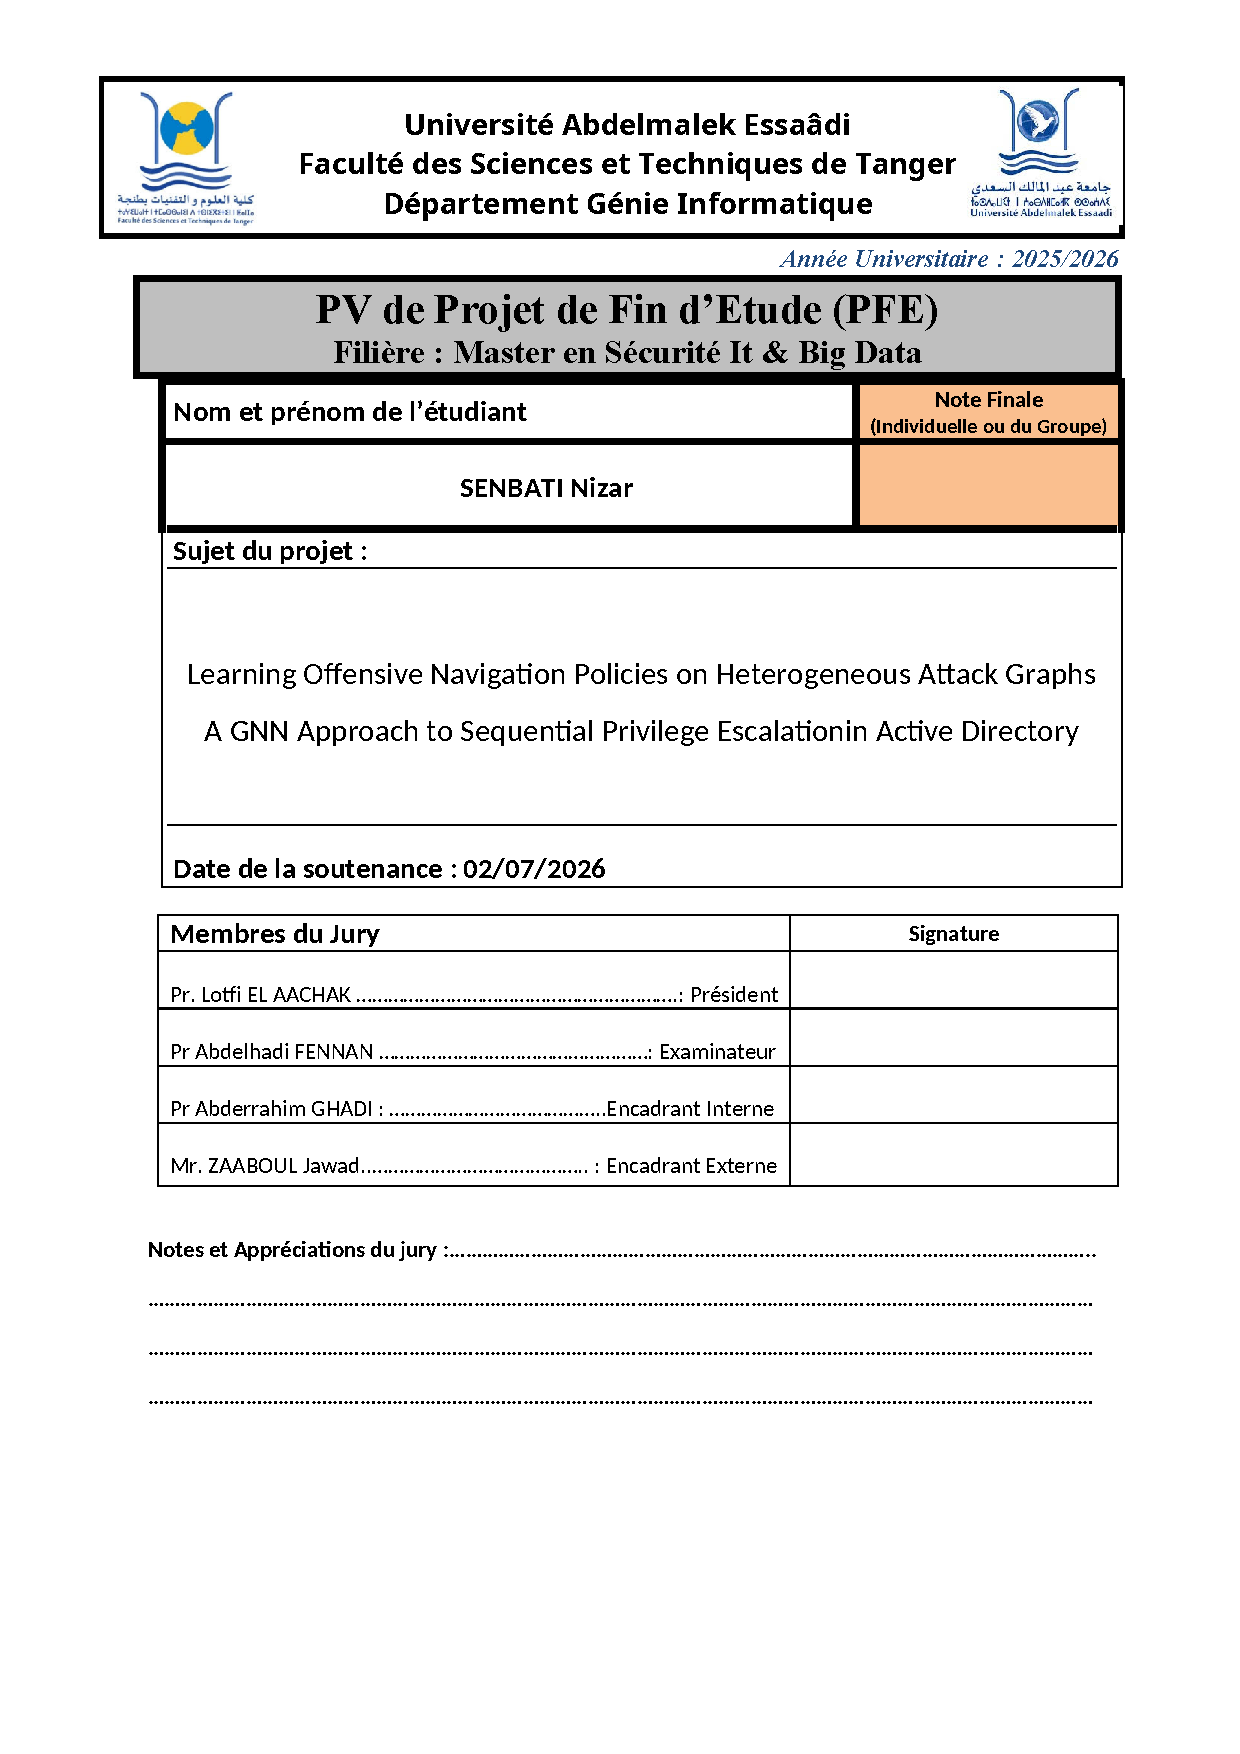
\includepdf[pages={1}]{ressources/pv.pdf}

\end{document}